\documentclass[12pt]{article}
\usepackage{geometry}
\usepackage{algorithm}
\usepackage{algorithmic}
\usepackage{amsmath}
\usepackage{parskip}
\usepackage{tikz}
\usepackage{amssymb}
\usepackage{hyperref}
\usepackage{pgfplots}
\pgfplotsset{compat=1.18}

\usetikzlibrary{positioning}

\geometry{margin=2cm} % or whatever size you prefer
%\setcounter{tocdepth}{1}
\begin{document}
\title{Machine Learning Study Guide}

\maketitle

\tableofcontents
\newpage


\section{ML Algorithms' Categories}
\subsection{Parametric and Non-Parametric Algorithms}

\textbf{Parametric Algorithms} assume that the data follows a specific distribution with a fixed number of parameters. Examples include linear regression and Gaussian Naive Bayes. Advantages include simplicity, speed, and less data requirement. However, they may suffer from limited flexibility and bias if the chosen model is incorrect.

\textbf{Non-Parametric Algorithms} do not assume any specific distribution for the data, learning the structure as they train. Examples include k-nearest neighbors and decision trees. They offer flexibility and fewer assumptions but may be complex, computationally intensive, and require more data.

Parametric algorithms are useful when the data distribution is clear and limited, while non-parametric algorithms are suitable when there's no prior knowledge about the data distribution or when the relationship between features and target variables is complex. Factors such as dataset size, computational resources, model interpretability, and problem nature should be considered when choosing between the two types of algorithms.

\subsection{Supervised, Self-Supervised, and Unsupervised Learning}
\textbf{Supervised Learning} involves training a model on labeled data, mapping inputs to target outputs. This approach excels in tasks such as image classification and speech recognition. However, it requires a substantial amount of labeled data, which can be costly and time-consuming to acquire.

\textbf{Self-Supervised Learning} leverages the structure of input data to create pseudo-labels, guiding the learning process. By solving a pretext task, the model learns representations transferable to various downstream tasks. While this approach capitalizes on unlabeled data, the quality of learned representations depends on the choice of pretext task, and it may be computationally expensive.

\textbf{Unsupervised Learning} focuses on capturing the underlying structure or distribution of data without relying on labels. Techniques such as clustering and dimensionality reduction are common in unsupervised learning. This paradigm also utilizes unlabeled data, but its applicability to specific tasks depends on the inherent structure of the data and the algorithm's ability to capture it.


\section{Distance Measures in Machine Learning}

Distance measures play a crucial role in many machine learning algorithms, such as clustering, nearest neighbor search, and dimensionality reduction. They quantify the similarity or dissimilarity between data points, which can be used to inform decisions made by algorithms.

\subsection{L1 Distance (Manhattan Distance)}

The L1 distance, also known as Manhattan distance or Taxicab distance, is the sum of the absolute differences between the coordinates of two points in a vector space. Given two vectors $\mathbf{x}$ and $\mathbf{y}$, the L1 distance is defined as:

$$d_{L1}(\mathbf{x}, \mathbf{y}) = \sum_{i=1}^{n} |x_i - y_i|$$

\subsection{L2 Distance (Euclidean Distance)}

The L2 distance, also known as Euclidean distance, is the square root of the sum of the squared differences between the coordinates of two points in a vector space. Given two vectors $\mathbf{x}$ and $\mathbf{y}$, the L2 distance is defined as:

$$d_{L2}(\mathbf{x}, \mathbf{y}) = \sqrt{\sum_{i=1}^{n} (x_i - y_i)^2}$$

\subsection{Cosine Distance}

Cosine distance is a measure of the angle between two vectors, and it is often used to compare the direction of the vectors rather than their magnitudes. Given two vectors $\mathbf{x}$ and $\mathbf{y}$, the cosine distance is defined as:

$$d_{\text{cosine}}(\mathbf{x}, \mathbf{y}) = 1 - \frac{\mathbf{x} \cdot \mathbf{y}}{||\mathbf{x}|| \cdot ||\mathbf{y}||}$$

\subsection{Dot Product}

The dot product is a measure of the projection of one vector onto another. It is not a distance measure in the strict sense, but it can be used to compute the similarity between two vectors. Given two vectors $\mathbf{x}$ and $\mathbf{y}$, the dot product is defined as:

$$\mathbf{x} \cdot \mathbf{y} = \sum_{i=1}^{n} x_i \cdot y_i$$

\subsection{KL Divergence}

Kullback-Leibler (KL) Divergence is a measure of the difference between two probability distributions. It is often used to compare the similarity between probability distributions in machine learning tasks. Given two probability distributions $P$ and $Q$, the KL divergence is defined as:

$$D_{KL}(P || Q) = \sum_{i} P(i) \log \frac{P(i)}{Q(i)}$$

\subsection{Comparison and Summary}

\begin{itemize}
\item \textbf{L1 distance} is robust to outliers and less sensitive to small differences between coordinates. It is often used in sparse data settings and can be more interpretable than other distance measures.
\item \textbf{L2 distance} is the most commonly used distance measure and is sensitive to differences in magnitude. It can be affected by outliers and may not be suitable for high-dimensional data due to the curse of dimensionality.
\item \textbf{Cosine distance} focuses on the angle between vectors, making it less sensitive to differences in magnitude. It is often used in text mining and information retrieval tasks, where the direction of the vectors (e.g., term frequency) is more important than their magnitudes.

\item \textbf{Dot Product} measures the projection of one vector onto another, and although it is not a distance measure itself, it can be used to assess similarity between vectors. It is commonly used in tasks involving high-dimensional data, such as collaborative filtering and image recognition.

\item \textbf{KL Divergence} measures the difference between two probability distributions and is particularly useful for comparing the similarity between distributions in tasks such as language modeling and anomaly detection. However, it is not symmetric, which means that $D_{KL}(P || Q) \neq D_{KL}(Q || P)$.
\end{itemize}

The choice of distance measure depends on the specific problem and the nature of the data at hand. L1 and L2 distances are general-purpose distance measures, with L1 being more robust to outliers and L2 being more sensitive to differences in magnitude. Cosine distance is useful for comparing the direction of vectors, making it well-suited for text and high-dimensional data. Dot product can be used to assess similarity in high-dimensional spaces, while KL Divergence is more specialized for comparing probability distributions. It is essential to consider these characteristics when selecting a distance measure for a particular machine learning task.

\section{Classic ML Algorithms}
\subsection{Linear Regression}

Linear regression is a parametric supervised learning algorithm used for modeling the relationship between a dependent variable (target) and one or more independent variables (features). The goal is to find the best-fitting line (or hyperplane in the case of multiple features) that minimizes the sum of the squared differences between the actual and predicted values.

\subsubsection{Formula}

The formula for a simple linear regression (one feature) is:

$$ y = \beta_0 + \beta_1 x $$
In multiple linear regression (multiple features), the formula is:

$$y = \beta_0 + \beta_1 x_1 + \beta_2 x_2 + \dots + \beta_n x_n $$
where:
\begin{itemize}
\item $y$ is the dependent variable (target)
\item $x_i$ are the independent variables (features)
\item $\beta_0$ is the intercept
\item $\beta_i$ are the coefficients
\end{itemize}

\subsubsection{Ordinary Least Squares (OLS)}

OLS is a popular method for estimating the coefficients in linear regression. It aims to minimize the sum of squared residuals:

$$ \min_{\beta_0, \beta_1, \dots, \beta_n} \sum_{i=1}^m (y_i - (\beta_0 + \beta_1 x_{i1} + \dots + \beta_n x_{in}))^2$$
The closed-form solution for the coefficients can be expressed as:

$$ \boldsymbol{\beta} = (\mathbf{X}^T\mathbf{X})^{-1}\mathbf{X}^T\mathbf{y} $$
where:
\begin{itemize}
\item $\mathbf{X}$ is the feature matrix with a column of ones for the intercept
\item $\mathbf{y}$ is the target vector
\item $\boldsymbol{\beta}$ is the vector of coefficients
\end{itemize}

\subsubsection{Advantages}
\begin{enumerate}
\item Simplicity: Linear regression is easy to understand and implement.
\item Interpretability: The coefficients provide insights into the relationship between features and the target.
\item Speed: It is computationally efficient.
\end{enumerate}

\subsubsection{Disadvantages}
\begin{enumerate}
\item Limited complexity: Assumes a linear relationship between features and target, which may not always be true.
\item Sensitivity to outliers: Outliers can significantly impact the model's performance.
\item Multicollinearity: The presence of highly correlated features can lead to unstable estimates of coefficients.
\end{enumerate}

\subsubsection{Context}
Linear regression is widely used for problems involving continuous target variables when the relationship between features and the target is assumed to be linear. It is a good starting point for understanding more complex models and serves as a baseline for evaluating other regression techniques.




\subsection{Logistic Regression}

Logistic regression is a parametric supervised learning algorithm used for binary classification problems. It models the probability of a data point belonging to a specific class using a logistic function (sigmoid function). The algorithm estimates the coefficients of the linear combination of features that best predict the log-odds of the target class.

\subsubsection{Sigmoid Function}

The logistic (sigmoid) function maps the input to a value between 0 and 1, representing the probability of the target class:

$$P(y=1 | \mathbf{x}) = \frac{1}{1 + e^{-(\beta_0 + \beta_1 x_1 + \dots + \beta_n x_n)}}$$
where:
\begin{itemize}
\item $P(y=1 | \mathbf{x})$ is the probability of the target class given the features
\item $x_i$ are the independent variables (features)
\item $\beta_0$ is the intercept
\item $\beta_i$ are the coefficients
\end{itemize}

\begin{figure}[h]
    \centering
    \includegraphics[scale=0.7]{./media/sigmoid.png}
    \caption{Sigmoid function}
    \label{fig:f_sigmoid}
\end{figure}

\subsubsection{Cost Function}

The cost function for logistic regression is derived from the cross-entropy loss. For a single data point, the cost function is:

$$ J(\boldsymbol{\beta}) = -[y \log(P(y=1 | \mathbf{x})) + (1 - y) \log(1 - P(y=1 | \mathbf{x}))] $$
For a dataset with $m$ data points, the cost function is the average of the individual costs:

$$J(\boldsymbol{\beta}) = -\frac{1}{m}\sum_{i=1}^m [y_i \log(P(y_i=1 | \mathbf{x}_i)) + (1 - y_i) \log(1 - P(y_i=1 | \mathbf{x}_i))]$$

\subsubsection{Gradient Descent}

To minimize the cost function, gradient descent is used to update the coefficients iteratively. The update rule for gradient descent is:

$$\boldsymbol{\beta} := \boldsymbol{\beta} - \alpha \nabla J(\boldsymbol{\beta})$$
where:
\begin{itemize}
\item $\boldsymbol{\beta}$ is the vector of coefficients
\item $\alpha$ is the learning rate
\item $\nabla J(\boldsymbol{\beta})$ is the gradient of the cost function with respect to the coefficients
\end{itemize}

\subsubsection{Advantages}
\begin{enumerate}
\item Probabilistic interpretation: Logistic regression provides the probability of a data point belonging to a specific class.
\item Ease of implementation: It is relatively simple to implement and can be regularized to prevent overfitting.
\item Computationally efficient: The algorithm is not computationally intensive compared to more complex models.
\end{enumerate}

\subsubsection{Disadvantages}
\begin{enumerate}
\item Linearity assumption: Assumes a linear relationship between features and the log-odds of the target class, which may not always be true.
\item Binary classification: It is primarily used for binary classification problems, although it can be extended to multi-class classification using techniques like one-vs-rest or one-vs-one.
\item Performance: More complex models like support vector machines or neural networks can outperform logistic regression in some cases.
\end{enumerate}

\subsubsection{Context}

Logistic regression is widely used for binary classification problems where the relationship between features and the target class can be assumed to be linear. It is a good starting point for classification problems and serves as a baseline for evaluating other classification techniques.



\subsection{Support Vector Machines}

Support Vector Machines (SVM) is a non-parametric supervised learning algorithm used for binary and multiclass classification problems. SVM aims to find the optimal hyperplane that maximizes the margin between the two classes in the feature space. In cases where the data is not linearly separable, SVM can use kernel functions to transform the feature space to a higher-dimensional space where a separating hyperplane can be found.

\subsubsection{Margin and Support Vectors}

The margin is the distance between the closest data points of different classes and the separating hyperplane. The goal of SVM is to maximize this margin. The data points on the edge of the margin are called support vectors.

\subsubsection{Optimization Problem}

The optimization problem for SVM can be formulated as follows:

$$\min_{\mathbf{w}, b} \frac{1}{2} ||\mathbf{w}||^2 $$
subject to:

$$ y_i (\mathbf{w}^T \mathbf{x}_i + b) \geq 1, \quad i = 1, \dots, m $$
where:
\begin{itemize}
\item $\mathbf{w}$ is the normal vector to the hyperplane
\item $b$ is the bias term
\item $\mathbf{x}_i$ are the feature vectors
\item $y_i \in {-1, 1}$ are the target class labels
\item $m$ is the number of data points
\end{itemize}

\begin{figure}[h]
    \centering
    \includegraphics[scale=2.5]{./media/svm.png}
    \caption{SVM}
    \label{fig:svm}
\end{figure}

\subsubsection{Kernel Functions}

In cases where the data is not linearly separable, SVM can use kernel functions to implicitly map the data to a higher-dimensional space. Popular kernel functions include:

\begin{itemize}
\item Linear kernel: $K(\mathbf{x}_i, \mathbf{x}_j) = \mathbf{x}_i^T \mathbf{x}_j$
\item Polynomial kernel: $K(\mathbf{x}_i, \mathbf{x}_j) = (\gamma \mathbf{x}_i^T \mathbf{x}_j + r)^d$
\item Radial basis function (RBF) kernel: $K(\mathbf{x}_i, \mathbf{x}_j) = \exp(-\gamma ||\mathbf{x}_i - \mathbf{x}_j||^2)$
\item Sigmoid kernel: $K(\mathbf{x}_i, \mathbf{x}_j) = \tanh(\gamma \mathbf{x}_i^T \mathbf{x}_j + r)$
\end{itemize}

where $\gamma$, $r$, and $d$ are kernel-specific parameters.

\subsubsection{Advantages}
\begin{enumerate}
\item Effective in high-dimensional spaces: SVM can handle a large number of features.
\item Robustness: Only the support vectors affect the decision boundary, making the model robust to outliers.
\item Flexibility: Kernel functions allow SVM to model non-linear decision boundaries.
\end{enumerate}

\subsubsection{Disadvantages}
\begin{enumerate}
\item Scalability: SVM is not well-suited for very large datasets due to its computational complexity.
\item Model interpretability: SVM models can be difficult to interpret, especially with non-linear kernel functions.
\item Sensitive to hyperparameters: The choice of kernel function and hyperparameters can have a significant impact on the model's performance.
\end{enumerate}

\subsubsection{Context}

SVM is widely used for classification problems when the relationship between features and the target class is complex or non-linear. It is effective in high-dimensional spaces and can handle a large number of features.


\subsection{Decision Trees}

Decision trees are non-parametric supervised learning algorithms used for both classification and regression tasks. They model the relationship between features and the target variable by recursively partitioning the input space and learning simple decision rules based on the features. Decision trees can be visualized as a flowchart-like structure, with internal nodes representing decisions based on feature values and leaf nodes representing the predicted target values.

\subsubsection{Nodes and Leaves}

\begin{itemize}
\item \textbf{Internal nodes}: Represent decisions based on feature values. Each internal node tests a specific feature and has multiple branches, each corresponding to a possible value or range of values for that feature.
\item \textbf{Leaf nodes}: Represent the predicted target value (class label for classification or continuous value for regression) associated with a specific combination of feature values.
\end{itemize}

\subsubsection{Training Algorithms}

There are various algorithms for constructing decision trees, such as ID3, C4.5, and CART. They generally use a greedy, top-down approach:

\begin{enumerate}
\item Select the best feature and split value based on a criterion (e.g., information gain, Gini impurity).
\item Partition the dataset into subsets based on the chosen feature and split value.
\item Recursively apply steps 1 and 2 on each subset until a stopping condition is met (e.g., maximum depth, minimum samples per leaf).
\end{enumerate}

\subsubsection{Inference}

Inference in decision trees involves traversing the tree from the root to a leaf node. At each internal node, the decision is made based on the value of the corresponding feature in the input data. The final prediction is obtained from the leaf node reached at the end of the traversal.

\subsubsection{Pruning}

Pruning is a technique used to reduce the complexity of a decision tree and mitigate overfitting. There are two main types of pruning:

\begin{itemize}
\item \textbf{Pre-pruning}: Stop growing the tree before it perfectly fits the training data, based on a stopping condition (e.g., maximum depth, minimum samples per leaf).
\item \textbf{Post-pruning}: First grow the tree to fit the training data, then iteratively remove branches that do not improve the tree's performance on a validation dataset.
\end{itemize}

\subsubsection{Advantages}
\begin{enumerate}
\item Interpretability: Decision trees are easy to understand and visualize, making them highly interpretable.
\item Minimal data preprocessing: Decision trees do not require feature scaling or normalization, and they can handle both numerical and categorical features.
\item Non-linear relationships: Decision trees can model complex, non-linear relationships between features and the target variable.
\end{enumerate}

\subsubsection{Disadvantages}
\begin{enumerate}
\item Overfitting: Decision trees can easily overfit the training data, especially when they are deep or have few samples per leaf.
\item Instability: Small changes in the training data can lead to significantly different trees, making decision trees sensitive to noise and variance.
\item Greedy nature: The greedy, top-down approach used in tree construction may not always result in the optimal tree, as it does not consider all possible trees.
\end{enumerate}

\subsubsection{Context}

Decision trees are widely used for problems where interpretability is important, and they can handle a mix of numerical and categorical features. They serve as the foundation for more advanced ensemble methods like random forests and gradient boosting machines.


\subsection{K-Means Clustering}
K-means clustering is a widely-used unsupervised learning algorithm for partitioning a dataset into a specified number of clusters (\textit{K}). The algorithm aims to minimize the within-cluster sum of squares (inertia) by iteratively updating the cluster centroids and cluster assignments.

\subsubsection{Algorithm}
The K-means clustering algorithm proceeds as follows:
\begin{enumerate}
\item Initialize the \textit{K} cluster centroids randomly by selecting \textit{K} data points from the dataset.
\item Assign each data point to the nearest centroid.
\item Update the centroids by computing the mean of all data points assigned to each centroid.
\item Repeat steps 2 and 3 until convergence (i.e., the centroids do not change significantly or a maximum number of iterations is reached).
\end{enumerate}

\subsubsection{Advantages}
Some advantages of K-means clustering include:
\begin{enumerate}
\item Simplicity and ease of implementation.
\item Efficient computation, making it suitable for large datasets.
\item Scalability to high-dimensional data when combined with dimensionality reduction techniques.
\item Wide applicability across various domains and tasks.
\end{enumerate}

\subsubsection{Disadvantages}
However, K-means clustering also has several disadvantages:
\begin{enumerate}
\item The need to specify the number of clusters (\textit{K}) beforehand, which may not be known a priori.
\item Sensitivity to initial centroid placement, potentially leading to different clustering results for different initializations.
\item Convergence to local optima, which can be mitigated by running the algorithm multiple times with different initializations.
\item The assumption of equal-sized and spherical clusters, which may not hold for real-world datasets.
\item Sensitivity to outliers and noise, which can be addressed by using robust variants of K-means or by preprocessing the data.
\end{enumerate}


\subsection{Hierarchical Clustering}
Hierarchical clustering is an unsupervised learning algorithm that builds a tree-like structure (dendrogram) to represent the nested grouping of data points based on their similarity. There are two main approaches to hierarchical clustering: agglomerative (bottom-up) and divisive (top-down).

\subsubsection{Algorithm}
The agglomerative hierarchical clustering algorithm proceeds as follows:
\begin{enumerate}
\item Treat each data point as a singleton cluster.
\item Compute the pairwise distances between all clusters.
\item Merge the two clusters with the smallest distance, creating a new cluster.
\item Update the distance matrix by calculating the distances between the new cluster and the remaining clusters using a linkage criterion (e.g., single, complete, average, or Ward's linkage).
\item Repeat steps 2 to 4 until there is only one cluster left, which contains all the data points.
\end{enumerate}

The divisive hierarchical clustering algorithm is less common and works by initially treating the entire dataset as a single cluster, then recursively splitting clusters into smaller clusters until each data point forms its own cluster.

\begin{figure}[h]
    \centering
    \includegraphics[scale=0.4]{./media/agg_clustering.png}
    \caption{Agglomerative Clustering}
    \label{fig:svm}
\end{figure}

\subsubsection{Advantages}
Some advantages of hierarchical clustering include:
\begin{enumerate}
\item No need to specify the number of clusters beforehand, as the dendrogram can be cut at different levels to obtain different clustering results.
\item The dendrogram provides a visual representation of the clustering process, aiding interpretation and understanding of the data structure.
\item Robustness to initialization, as the algorithm is deterministic and does not depend on random initial conditions.
\item Ability to handle non-spherical and non-convex clusters by using appropriate distance and linkage measures.
\end{enumerate}

\subsubsection{Disadvantages}
However, hierarchical clustering also has several disadvantages:
\begin{enumerate}
\item Higher computational complexity compared to K-means, making it less suitable for large datasets.
\item Irreversibility of the clustering process, meaning that once clusters are merged (agglomerative) or split (divisive), they cannot be undone in subsequent steps.
\item Sensitivity to the choice of distance and linkage measures, which can affect the clustering results.
\item Difficulty in determining the optimal number of clusters and the appropriate cutting level in the dendrogram.
\end{enumerate}

\subsection{DBSCAN}
Density-Based Spatial Clustering of Applications with Noise (DBSCAN) is an unsupervised clustering algorithm that groups data points based on their density in the feature space. Unlike K-means and hierarchical clustering, DBSCAN does not require the user to specify the number of clusters beforehand and is capable of handling noise and identifying clusters of arbitrary shapes.

\subsubsection{Algorithm}
\begin{enumerate}
\item For each unvisited data point, retrieve its neighborhood, which consists of all points within a specified distance $\epsilon$ (eps) from the point.
\item If the neighborhood contains at least a minimum number of points (minPts), consider the data point as a core point and form a cluster. Recursively expand the cluster by adding all directly density-reachable points and their respective density-reachable points.
\item If the data point is not a core point and not density-reachable from any core point, label it as noise.
\item Repeat steps 1 to 3 until all data points have been visited and assigned to a cluster or labeled as noise.
\end{enumerate}

\subsubsection{Advantages}
\begin{enumerate}
\item No need to specify the number of clusters beforehand, as the algorithm automatically determines the number of clusters based on the density of the data points.
\item Ability to identify clusters of arbitrary shapes, as opposed to K-means, which is limited to spherical clusters.
\item Robustness to noise, as the algorithm explicitly labels and separates noise points from the clusters.
\item Deterministic clustering results, as long as the order of processing the data points is fixed.
\end{enumerate}

\subsubsection{Disadvantages}
\begin{enumerate}
\item Sensitivity to the choice of $\epsilon$ and minPts parameters, which can significantly affect the clustering results.
\item Difficulty in determining the optimal values for $\epsilon$ and minPts, especially for datasets with varying densities.
\item Poor performance on high-dimensional data due to the curse of dimensionality, which affects the density estimation.
\item Inefficient for large datasets, as the algorithm has a quadratic time complexity in the worst case.
\end{enumerate}
DBSCAN can find arbitrarily shaped clusters, is robust to noise, and does not require the number of clusters to be specified beforehand. However, it is sensitive to the choice of hyperparameters ($\varepsilon$ and $\text{MinPts}$) and may not perform well when clusters have varying densities.
\subsection{PCA (Principal Component Analysis)}
Principal Component Analysis (PCA) is a dimensionality reduction technique used to transform a high-dimensional dataset into a lower-dimensional space while preserving the maximum amount of variance in the data. PCA is particularly useful for visualization, data compression, and improving the efficiency of other machine learning algorithms.

The main steps involved in PCA are as follows:

\begin{enumerate}
\item Standardize the data by centering the features around their mean and scaling them to have unit variance.
\item Compute the covariance matrix of the standardized data.
\item Calculate the eigenvalues and eigenvectors of the covariance matrix.
\item Sort the eigenvectors in descending order of their corresponding eigenvalues.
\item Select the first $k$ eigenvectors with the highest eigenvalues to form a $d \times k$ dimensional projection matrix, where $d$ is the original dimensionality and $k$ is the target dimensionality.
\item Transform the original data by multiplying it with the projection matrix to obtain the lower-dimensional representation.
\end{enumerate}
PCA assumes that the principal components are linear combinations of the original features and works well when the data has a linear structure. However, it may not capture complex, nonlinear relationships between the features.

\subsection{t-SNE (t-Distributed Stochastic Neighbor Embedding)}
t-SNE is a non-linear dimensionality reduction technique particularly suited for visualizing high-dimensional data in a 2D or 3D space. It is based on the concept of preserving the local distances between instances in the lower-dimensional space, making it effective for revealing clusters and structures in the data.

\begin{enumerate}
\item Define a probability distribution over pairs of instances in the high-dimensional space such that similar instances have a higher probability of being picked, while dissimilar instances have a lower probability. This is usually done by modeling the pairwise similarities using a Gaussian distribution.
\item Define a probability distribution over pairs of instances in the lower-dimensional space using a t-distribution with one degree of freedom (also known as the Student's t-distribution).
\item Minimize the Kullback-Leibler (KL) divergence between the two probability distributions with respect to the lower-dimensional embeddings using gradient descent. The KL divergence is a measure of how one probability distribution is different from another.
\end{enumerate}
t-SNE has some advantages over PCA, as it can capture non-linear structures in the data and is more effective at visualizing clusters. However, it is computationally expensive and does not provide an explicit mapping function between the high-dimensional and low-dimensional spaces, making it unsuitable for out-of-sample data.

\section{Ensemble Methods}

Ensemble methods are techniques that combine multiple base learners to create a more powerful and accurate model. They can be used with various types of base learners, such as decision trees, logistic regression, or support vector machines. There are two main types of ensemble methods: bagging and boosting.

\subsection{Bagging}

Bagging (Bootstrap Aggregating) is an ensemble method that trains multiple base learners independently on different subsets of the training data, generated by random sampling with replacement (bootstrap samples). The final prediction is obtained by averaging (for regression) or voting (for classification) the predictions of all base learners.

\subsubsection{Random Forests}
Random Forests is an ensemble learning method that builds multiple decision trees and combines their predictions to improve the overall performance and robustness of the model. It is primarily used for both classification and regression tasks.

\paragraph{Algorithm}
The Random Forests algorithm works as follows:
\begin{enumerate}
\item Select a random subset of the data with replacement (bootstrap sample) to build each decision tree.
\item For each decision tree, at each split node, select a random subset of features and use the best split criterion (e.g., Gini impurity or information gain) to split the node.
\item Grow each decision tree to its maximum depth, without pruning.
\item Make a prediction for each decision tree in the ensemble.
\item Combine the predictions from all decision trees using majority voting (classification) or averaging (regression) to obtain the final prediction.
\end{enumerate}

\paragraph{Advantages}
Some advantages of Random Forests include:
\begin{enumerate}
\item High predictive accuracy due to the combination of multiple decision trees, which helps to reduce overfitting and improve generalization.
\item Robustness to noise and outliers, as each decision tree is trained on a random subset of the data and features, making the overall model less sensitive to individual data points.
\item Ability to handle large datasets with many features and missing values.
\item Provides feature importance scores, which can be used for feature selection and understanding the underlying structure of the data.
\end{enumerate}

\paragraph{Disadvantages}
However, Random Forests also has several disadvantages:
\begin{enumerate}
\item Increased computational complexity and memory requirements due to the construction and storage of multiple decision trees.
\item Slower prediction times compared to single decision trees, as predictions from all trees in the ensemble must be combined.
\item Reduced interpretability compared to single decision trees, as the ensemble model is more complex and harder to visualize.
\end{enumerate}


\subsection{Boosting}

Boosting is an ensemble method that trains multiple base learners sequentially, with each learner focusing on the errors made by the previous one. The final prediction is obtained by combining the predictions of all base learners, typically using a weighted average or a weighted vote.

\subsubsection{AdaBoost}

AdaBoost (Adaptive Boosting) is a boosting algorithm that uses decision stumps (one-level decision trees) as base learners. AdaBoost adjusts the weights of the training samples based on the errors made by the previous learner and trains the next learner on the reweighted samples. The final prediction is a weighted vote of all base learners, with the weights determined by their classification accuracy.

\subsubsection{Gradient Boosting Machine}
Gradient Boosting Machine (GBM) is an ensemble learning method that builds a series of weak learners, often decision trees, and combines them to form a strong learner. The main idea behind GBM is to iteratively train weak learners to correct the errors made by the previous learners in the ensemble. It is mainly used for regression and classification tasks.

\paragraph{Algorithm}
The Gradient Boosting Machine algorithm works as follows:
\begin{enumerate}
\item Initialize the model with a constant prediction value, typically the mean of the target variable for regression or the majority class for classification.
\item For each iteration, fit a weak learner (e.g., a shallow decision tree) to the residuals (the difference between the true target values and the current predictions) of the previous iteration.
\item Update the predictions by adding a fraction of the weak learner's predictions to the current predictions. This fraction, called the learning rate, controls the contribution of each weak learner to the ensemble.
\item Repeat steps 2-3 for a predefined number of iterations or until a convergence criterion is met.
\end{enumerate}

\paragraph{Advantages}
Some advantages of Gradient Boosting Machine include:
\begin{enumerate}
\item High predictive accuracy due to the combination of multiple weak learners, which helps to reduce overfitting and improve generalization.
\item Flexibility, as it can work with various loss functions and different types of weak learners, not limited to decision trees.
\item Robustness to noise and outliers, as each weak learner is trained on the residuals of the previous learners, making the overall model less sensitive to individual data points.
\item Provides feature importance scores, which can be used for feature selection and understanding the underlying structure of the data.
\end{enumerate}

\paragraph{Disadvantages}
However, Gradient Boosting Machine also has several disadvantages:
\begin{enumerate}
\item Increased computational complexity and longer training times due to the sequential nature of the algorithm, which makes it harder to parallelize compared to other ensemble methods like Random Forests.
\item Requires careful tuning of hyperparameters, such as the number of iterations, learning rate, and tree depth, to achieve optimal performance.
\item Reduced interpretability compared to single decision trees, as the ensemble model is more complex and harder to visualize.
\end{enumerate}

\paragraph{Intuition}
The intuition behind Gradient Boosting Machine is to iteratively improve the model's predictions by focusing on the errors made in previous iterations. By training weak learners on the residuals, GBM forces each new learner to focus on the areas where the current ensemble is performing poorly. This process can be thought of as a way to "correct" the mistakes made by the previous learners, allowing the ensemble to gradually improve its predictions over time. The learning rate parameter helps to control the pace at which the model learns, preventing overfitting and ensuring that each weak learner makes a modest contribution to the overall model.

\subsubsection{XGBoost}

XGBoost (eXtreme Gradient Boosting) is an optimized version of GBM that introduces several improvements, such as:

\begin{itemize}
\item Regularization: XGBoost includes L1 and L2 regularization terms in the loss function to prevent overfitting.
\item Sparsity-aware: XGBoost can handle sparse data and missing values efficiently.
\item Column block: XGBoost uses a compressed memory-efficient representation of the input data, which speeds up training and inference.
\item Parallelization: XGBoost parallelizes the construction of decision trees across multiple CPU cores.
\end{itemize}

\subsection{Advantages}
\begin{enumerate}
\item Improved accuracy: Ensemble methods typically achieve better performance than single base learners.
\item Robustness: Ensembles are more robust to noise and outliers, as they combine the predictions of multiple base learners.
\item Flexibility: Ensemble methods can be used with various types of base learners and can be adapted for different tasks (classification, regression).
\end{enumerate}

\subsection{Disadvantages}
\begin{enumerate}
\item Increased complexity: Ensemble methods can be more complex and harder to interpret than single base learners, especially with boosting algorithms.
\item Computational cost: Training and inference with ensemble methods can be computationally expensive, as they involve multiple base learners.
\item Risk of overfitting: Boosting algorithms, in particular, can be prone to overfitting if the base learners are too complex or the number of boosting iterations is too high.
\end{enumerate}


\section{Optimization}

Optimization refers to the process of finding the best set of parameters for a machine learning model to minimize the objective function (e.g., the loss function). Gradient-based optimization algorithms use the gradient of the objective function to update the model parameters iteratively until a local minimum is reached.

\subsection{Gradient Descent}

Gradient descent is a first-order optimization algorithm that updates the model parameters based on the gradient of the objective function:

$$\boldsymbol{\theta} := \boldsymbol{\theta} - \alpha \nabla J(\boldsymbol{\theta})$$
where:
\begin{itemize}
\item $\boldsymbol{\theta}$ is the vector of model parameters
\item $\alpha$ is the learning rate
\item $\nabla J(\boldsymbol{\theta})$ is the gradient of the objective function with respect to the parameters
\end{itemize}

\subsection{Stochastic Gradient Descent (SGD)}

Stochastic Gradient Descent (SGD) is a variant of gradient descent that updates the model parameters based on the gradient of the objective function computed for a single data point or a small batch of data points:

$$\boldsymbol{\theta} := \boldsymbol{\theta} - \alpha \nabla J(\boldsymbol{\theta}; \mathbf{x}_i, y_i)$$
where $(\mathbf{x}_i, y_i)$ is a single data point or a small batch of data points.

\subsubsection{Advantages of Stochastic Gradient Descent}

\begin{itemize}
\item \textbf{Faster convergence:} Since the gradient is computed using only a small portion of the dataset, the computation is significantly faster, which allows for quicker updates to the model's parameters. This can lead to faster convergence to the optimal solution, especially when dealing with large datasets.

\item \textbf{Noise can help escape local minima:} The inherent noise in the stochastic gradient estimate can actually help the algorithm escape local minima in non-convex optimization problems. This characteristic can be beneficial in deep learning models where the loss surface may have many local minima.

\item \textbf{Memory efficiency:} SGD requires less memory compared to full-batch Gradient Descent since only a small portion of the dataset is loaded into memory at a time. This makes it possible to train models on large datasets that may not fit entirely into memory.

\item \textbf{Tunable trade-off between computation and convergence:} By adjusting the batch size used in SGD, one can control the trade-off between computational efficiency and convergence rate. Smaller batch sizes will result in faster updates but may lead to a noisier convergence, while larger batch sizes can provide a more stable convergence but at a higher computational cost.
\end{itemize}


\subsection{Momentum}

Momentum is a technique that accelerates gradient descent and helps overcome local minima by introducing a velocity term, which is the exponentially decaying moving average of the gradients:

\begin{align*}
\mathbf{v} &= \gamma \mathbf{v} + \alpha \nabla J(\boldsymbol{\theta}) \\
\boldsymbol{\theta} &= \boldsymbol{\theta} - \mathbf{v}\\
\end{align*}
where $\gamma$ is the momentum coefficient (typically between 0.9 and 0.99).

The momentum term increases for dimensions whose gradients point in the same directions and reduces updates for dimensions whose gradients change directions. As a result, we gain faster convergence and reduced oscillation.

\subsection{AdaGrad}

\textbf{Gradient Accumulation:}
\[
G_{t,i} = \sum_{k=1}^{t} g_{k,i}^2
\]

\textbf{Parameter Update:}
\[
\theta_{t+1,i} = \theta_{t,i} - \frac{\eta}{\sqrt{G_{t,i}} + \epsilon} g_{t,i}
\]

where:
\begin{itemize}
    \item \( \theta_{t,i} \) is the current parameter.
    \item \( \theta_{t+1,i} \) is the updated parameter.
    \item \( \eta \) is the learning rate.
    \item \( g_{k,i} \) is the gradient of the loss function with respect to parameter \( \theta_i \) at step \( k \).
    \item \( G_{t,i} \) is the accumulated sum of squared gradients up to time \( t \).
    \item \( \epsilon \) is a small constant for numerical stability (typically \( 10^{-8} \)).
\end{itemize}

\textbf{Diminishing Learning Rates}:
   \begin{itemize}
       \item The accumulated sum of squared gradients \( G_{t,i} \) keeps growing over time.
       \item This leads to the learning rates becoming very small, which can slow down convergence significantly or cause the training to stop prematurely.
   \end{itemize}

\subsection{RMSprop}

RMSprop (Root Mean Square Propagation) is an optimization algorithm that adapts the learning rate for each parameter based on the moving average of the squared gradients:

\begin{align*}
	\mathbf{s} &:= \rho \mathbf{s} + (1 - \rho) (\nabla J(\boldsymbol{\theta}))^2\\
\boldsymbol{\theta} &:= \boldsymbol{\theta} - \frac{\alpha}{\sqrt{\mathbf{s} + \epsilon}} \nabla \\J(\boldsymbol{\theta})
\end{align*}
where $\rho$ is the decay rate (typically between 0.9 and 0.99), and $\epsilon$ is a small constant to prevent division by zero.

RMSprop addresses the limitation of AdaGrad by using a moving average of the squared gradients instead of the cumulative sum. This prevents the learning rate from diminishing too quickly, ensuring that the optimization process remains effective throughout the training. The moving average allows RMSprop to maintain a more balanced and consistent learning rate, leading to better performance, especially in non-stationary settings.

\subsection{ADAM}

ADAM (Adaptive Moment Estimation) is an optimization algorithm for gradient-based optimization of neural networks and other machine learning models. It is an extension of stochastic gradient descent (SGD) that combines the benefits of adaptive learning rates and momentum. ADAM is widely used in deep learning due to its efficiency and robustness.

\begin{align*}
m_t &= \beta_1 m_{t-1} + (1 - \beta_1) \nabla J(\boldsymbol{\theta}{t-1}) \\
v_t &= \beta_2 v{t-1} + (1 - \beta_2) (\nabla J(\boldsymbol{\theta}_{t-1}))^2 \\
\hat{m}_t &= \frac{m_t}{1 - \beta_1^t} \\
\hat{v}_t &= \frac{v_t}{1 - \beta_2^t} \\
\boldsymbol{\theta}t &= \boldsymbol{\theta}{t-1} - \alpha \frac{\hat{m}_t}{\sqrt{\hat{v}_t} + \epsilon}
\end{align*}



where:
\begin{itemize}
\item $\boldsymbol{\theta}$ is the parameter vector
\item $\nabla J(\boldsymbol{\theta})$ is the gradient of the objective function with respect to the parameters
\item $m_t$ and $v_t$ are the first and second moment estimates, respectively
\item $\beta_1$ and $\beta_2$ are the exponential decay rates for the first and second moment estimates (usually set to 0.9 and 0.999)
\item $\alpha$ is the learning rate
\item $\epsilon$ is a small constant to prevent division by zero (usually set to $10^{-8}$)
\item $t$ is the iteration number
\end{itemize}

\subsubsection{Intuition}

ADAM combines the ideas of adaptive learning rates and momentum:

\begin{itemize}
\item \textbf{Adaptive learning rates}: ADAM computes individual learning rates for each parameter based on the square root of the second moment estimate ($\hat{v}_t$). This allows the algorithm to adapt the learning rate for each parameter based on the scale and sparsity of the gradients, which can help with convergence and stability.
\item \textbf{Momentum}: ADAM maintains a moving average of the gradients (first moment estimate $m_t$) to incorporate information from past gradients. This helps to accelerate the convergence and overcome local minima or noisy gradients.
\end{itemize}

\section{Loss Functions}

Loss functions measure the difference between the predictions made by a machine learning model and the true target values. They are used during the training process to update the model's parameters to minimize the loss. Here, we discuss three commonly used loss functions: logistic loss, cross-entropy loss, and hinge loss.

\subsection{Logistic Loss}

The logistic loss, also known as the log loss or binary cross-entropy loss, is used in binary classification problems. It is defined as:

$$L(y, p) = -y \log(p) - (1 - y) \log(1 - p)$$
where:
\begin{itemize}
\item $y$ is the true class label (0 or 1)
\item $p$ is the predicted probability of the positive class (1)
\end{itemize}

\subsubsection{Intuition}

The logistic loss penalizes wrong predictions with a logarithmic scale, where the penalty increases as the predicted probability deviates from the true class label. When the predicted probability is close to the true label, the loss is small, while the loss becomes large when the predicted probability is far from the true label. This encourages the model to assign high confidence to the correct class.

\subsection{Cross-Entropy Loss}

The cross-entropy loss, also known as categorical cross-entropy loss, is used in multiclass classification problems. It is defined as:

$$L(\boldsymbol{y}, \boldsymbol{p}) = -\sum_{i=1}^{C} y_i \log(p_i)$$
where:
\begin{itemize}
\item $\boldsymbol{y}$ is the one-hot encoded true class label vector
\item $\boldsymbol{p}$ is the predicted probability vector for each class
\item $C$ is the number of classes
\item $y_i$ and $p_i$ are the true label and predicted probability, respectively, for class $i$
\end{itemize}

\subsubsection{Intuition}

The cross-entropy loss is an extension of the logistic loss for multiclass problems. It measures the dissimilarity between the true class label distribution and the predicted probability distribution. Like logistic loss, the cross-entropy loss penalizes wrong predictions with a logarithmic scale, encouraging the model to assign high confidence to the correct class.

\subsection{Hinge Loss}

The hinge loss is used in support vector machines (SVM) for binary classification problems. It is defined as:

$$L(y, f(\boldsymbol{x})) = \max(0, 1 - y f(\boldsymbol{x}))$$
where:
\begin{itemize}
\item $y$ is the true class label (-1 or 1)
\item $f(\boldsymbol{x})$ is the raw output of the SVM, representing the signed distance from the input data point $\boldsymbol{x}$ to the decision boundary
\end{itemize}

\subsubsection{Intuition}

The hinge loss encourages a margin between the two classes in the feature space. It penalizes predictions that fall within the margin or on the wrong side of the decision boundary. The loss is zero for points that lie outside the margin and on the correct side of the boundary, which means that the model focuses on improving the predictions for the most difficult samples (those that are close to the decision boundary). This is consistent with the objective of SVMs to find the maximum-margin hyperplane that separates the classes.

\subsection{Triplet Loss}

Triplet loss is designed to optimize the relative distance between anchor, positive, and negative examples in the embedding space. Given a dataset with $N$ samples, each sample is represented as a triple $(a, p, n)$, where $a$ is the anchor, $p$ is a positive example with the same identity or class as the anchor, and $n$ is a negative example from a different identity or class. The triplet loss function is defined as:

\begin{equation}
\mathcal{L}(a, p, n) = \max\left\{d(a, p) - d(a, n) + \alpha, 0\right\}
\end{equation}

where $d(a, b)$ denotes the distance metric, usually the Euclidean distance, between embeddings $a$ and $b$, and $\alpha$ is the margin. The goal is to minimize the total triplet loss:

\begin{equation}
\mathcal{L}_{total} = \sum_{i=1}^{N} \mathcal{L}(a_i, p_i, n_i)
\end{equation}

\subsubsection{Hyperparameters}

\begin{itemize}
\item \textbf{Margin ($\alpha$):} The margin enforces a minimum separation between positive and negative pairs in the embedding space. A suitable value of $\alpha$ is critical for the convergence and performance of the model. A margin prevents the model from learning trivial solutions where all embeddings collapse to a single point or become very close to each other. This is because the model has to ensure that the anchor-positive distance is always smaller than the anchor-negative distance by at least $\alpha$. It also enforces the separation between different classes in the embedding space, leading to embeddings with higher discriminative power.
\item \textbf{Batch size:} The batch size influences the number of triplets used in each iteration of the optimization process. A larger batch size may lead to more stable optimization, but can also increase computational requirements.
\end{itemize}

\subsubsection{Hard Negative Mining}

Hard negative mining is a strategy used to improve the convergence and performance of the model by selecting more challenging negative examples. In the context of triplet loss, hard negatives are those instances for which the difference in distances, $d(a, p) - d(a, n)$, is small. By focusing on hard negatives, the model is encouraged to learn more discriminative embeddings.

Two common approaches to hard negative mining are:

\begin{enumerate}
\item \textbf{Batch hard negative mining:} For each anchor-positive pair in a mini-batch, select the hardest negative example, i.e., the one with the smallest distance to the anchor.
\item \textbf{Online hard negative mining:} Continuously update the negative examples during training, selecting the hardest negatives for each anchor-positive pair at each iteration.
\end{enumerate}

\subsection{Mean Squared Error (MSE)}

The mean squared error (MSE) is a widely used loss function for regression tasks. It is defined as:

$$L(\boldsymbol{y}, \boldsymbol{\hat{y}}) = \frac{1}{N} \sum_{i=1}^{N} (y_i - \hat{y}_i)^2$$

\subsubsection{Intuition}

The MSE measures the average squared difference between the true and predicted target values. It penalizes large errors more severely than small errors due to the squaring operation. This encourages the model to fit the data more closely and is sensitive to outliers.

\subsection{Mean Absolute Error (MAE)}

The mean absolute error (MAE) is another common loss function for regression tasks. It is defined as:
$$ L(\boldsymbol{y}, \boldsymbol{\hat{y}}) = \frac{1}{N} \sum_{i=1}^{N} |y_i - \hat{y}_i|$$
\subsubsection{Intuition}

The MAE measures the average absolute difference between the true and predicted target values. Unlike MSE, it does not penalize large errors as severely due to the absence of the squaring operation. This makes the MAE more robust to outliers and can be a better choice for problems with noisy or skewed data.


\section{Feature Selection}

Feature selection is the process of selecting a subset of the most important features from the original set of features in a dataset. It is an essential step in machine learning as it can improve model performance, reduce overfitting, and decrease training time. There are three main categories of feature selection methods: filter methods, wrapper methods, and embedded methods.

\subsection{Filter Methods}

Filter methods are based on the intrinsic properties of the features and their relationship with the target variable. They are independent of any specific machine learning model and are computationally efficient. Some common filter methods are:

\begin{itemize}
\item \textbf{Variance Threshold}: Features with low variance are removed, as they do not contribute much information to the model.
\item \textbf{Correlation Coefficient}: Features that have a high correlation with the target variable are selected, while features with a high correlation among themselves are removed to reduce multicollinearity.
\item \textbf{Mutual Information}: Features that have a high mutual information with the target variable are selected, as they share more information about the target variable.
\item \textbf{Chi-Squared Test}: In classification problems, the chi-squared test is used to measure the dependence between categorical features and the target variable. Features with high chi-squared values are more likely to be related to the target variable.
\end{itemize}

\subsection{Wrapper Methods}

Wrapper methods involve training a specific machine learning model with different feature subsets and selecting the subset that results in the best model performance. Although they can lead to better feature subsets, they are computationally expensive and prone to overfitting. Some common wrapper methods are:

\begin{itemize}
\item \textbf{Forward Selection}: Features are added one by one to the model, and the performance is evaluated at each step. The process stops when adding more features does not improve the performance.
\item \textbf{Backward Elimination}: Features are removed one by one from the model, and the performance is evaluated at each step. The process stops when removing more features degrades the performance.
\item \textbf{Recursive Feature Elimination}: A model is trained with all features, and the least important features are removed iteratively based on their importance. This process continues until the desired number of features is reached.
\end{itemize}
\subsection{Embedded Methods}
Embedded methods combine the advantages of both filter and wrapper methods by incorporating feature selection as part of the model training process. Some common embedded methods are:

\begin{itemize}
\item \textbf{Lasso Regression}: Lasso regression is a linear regression model with an L1 regularization term that encourages sparsity in the model parameters. It can be used to perform feature selection by setting the coefficients of irrelevant features to zero.
\item \textbf{Ridge Regression}: Ridge regression is a linear regression model with an L2 regularization term that discourages large parameter values. Although it does not perform feature selection directly, it can be useful for ranking features based on their coefficients.
\item \textbf{Elastic Net}: Elastic Net is a linear regression model that combines both L1 and L2 regularization terms. It can perform feature selection like Lasso while maintaining the stability of Ridge regression.
\item \textbf{Decision Trees}: Decision tree algorithms, such as CART and C4.5, can inherently perform feature selection by selecting the most important features at the top of the tree based on information gain or Gini impurity.
\item \textbf{Random Forests and Gradient Boosting Machines}: Ensemble methods like Random Forests and Gradient Boosting Machines can rank features based on their importance.
\end{itemize}

\section{Feature Scaling}
Feature scaling is an important preprocessing step that helps to bring the features of a dataset to a similar scale. This is crucial for many machine learning algorithms that are sensitive to the scale of input features, such as gradient descent-based methods, support vector machines, and k-means clustering. There are several techniques for feature scaling:

\subsection{Normalization}
Normalization, also known as min-max scaling, scales the features to a range of [0, 1]. The formula for normalization is as follows:
\begin{equation}
x_{normalized} = \frac{x - x_{min}}{x_{max} - x_{min}}
\end{equation}
where $x_{normalized}$ is the normalized value of feature $x$, $x_{min}$ and $x_{max}$ are the minimum and maximum values of the feature, respectively.

\subsection{Standardization}
Standardization scales the features so that they have a mean of 0 and a standard deviation of 1. This technique is useful when the features follow a Gaussian distribution. The formula for standardization is:
\begin{equation}
x_{standardized} = \frac{x - \mu}{\sigma}
\end{equation}
where $x_{standardized}$ is the standardized value of feature $x$, $\mu$ is the mean of the feature, and $\sigma$ is the standard deviation of the feature.

\subsection{Robust Scaling}
Robust scaling is a method that scales the features based on the median and interquartile range (IQR), making it robust to outliers. The formula for robust scaling is:
\begin{equation}
x_{robust} = \frac{x - Q_{1}}{Q_{3} - Q_{1}}
\end{equation}
where $x_{robust}$ is the robust-scaled value of feature $x$, $Q_{1}$ is the first quartile (25th percentile) of the feature, and $Q_{3}$ is the third quartile (75th percentile) of the feature.

\subsection{When to Use Feature Scaling}
Feature scaling is essential for algorithms that rely on the distance between data points, like k-means clustering and k-nearest neighbors, as well as for models that use gradient descent for optimization, such as linear regression and neural networks. It is less important for tree-based models like decision trees and random forests, as they are less sensitive to the scale of input features.

\section{Handling Categorical Variables}
Categorical variables are non-numeric data types that represent discrete categories or labels. Many machine learning algorithms require numeric input, so it is essential to convert categorical variables into a suitable numeric representation. There are several techniques for handling categorical variables:

\subsection{Label Encoding}
Label encoding assigns an integer value to each unique category. This method is useful when dealing with ordinal categorical variables, where the order of the categories is meaningful. However, it might not be suitable for nominal categorical variables, as the integer values can introduce an artificial order that does not exist in the data.

\subsection{One-Hot Encoding}
One-hot encoding creates binary features for each category of a categorical variable. For a variable with $k$ categories, one-hot encoding generates $k$ new binary features, with each feature representing the presence (1) or absence (0) of a specific category. This method is suitable for nominal categorical variables, as it does not introduce an artificial order. However, it can significantly increase the dimensionality of the dataset, especially if the categorical variables have many unique categories.

\subsection{Dummy Encoding}
Dummy encoding is similar to one-hot encoding but generates $k-1$ binary features for a variable with $k$ categories. This method helps to avoid the dummy variable trap, a situation where multicollinearity occurs due to the inclusion of redundant information in the dataset.

\subsection{Target Encoding}
Target encoding, also known as mean encoding, replaces the categorical variable with the mean of the target variable for each category. This method can capture the relationship between the categorical variable and the target variable while reducing the dimensionality of the dataset. However, it might introduce leakage if not done correctly, so it is essential to perform target encoding separately for the training and validation/test sets.

\subsection{Embeddings}
Embeddings are another way to represent categorical variables, especially when dealing with high cardinality categorical variables. Embeddings map categorical variables to low-dimensional vectors that can capture complex relationships between categories. This method is commonly used with deep learning models, such as neural networks and transformers.


\section{Model Architectures}

\subsection{Two-Tower Architecture for Search}

The two-tower architecture is a neural network design pattern commonly used in information retrieval tasks, such as search and recommendation systems. This architecture consists of two separate neural networks, or "towers," which are trained to generate embeddings for queries and documents (or items). The main advantage of this architecture is its ability to efficiently compute similarity scores between queries and documents in the embedding space, enabling fast and accurate retrieval of relevant items.

\subsubsection{Architecture Overview}

In a two-tower architecture, the query tower and the document tower have separate neural network structures that are tailored to their specific input types (e.g., text, images, or a combination of features). These towers can be constructed using various neural network components, such as fully connected layers, convolutional layers, or transformer layers, depending on the input data and the desired complexity of the model.

The query tower processes the user's query and generates a query embedding, while the document tower processes the documents or items and generates document embeddings. Once the embeddings are generated, they can be compared using a similarity metric, such as the dot product, cosine similarity, or Euclidean distance, to rank the documents according to their relevance to the query.

\subsubsection{Training the Two-Tower Model}

To train a two-tower model, the objective is to minimize a loss function that encourages the query and document embeddings to be similar when they are relevant to each other and dissimilar otherwise. One common approach is to use a ranking loss function, such as the triplet loss or the contrastive loss, which operates on pairs or triplets of query-document combinations with varying degrees of relevance.

During training, the query and document towers learn to generate embeddings that satisfy the desired similarity constraints. This is achieved by updating the model parameters using backpropagation and gradient descent, typically in a mini-batch setting. The trained model can then be used to generate query and document embeddings for information retrieval tasks, such as search and recommendation.

\subsubsection{Advantages for Search}

The two-tower architecture offers several benefits for search applications:
\begin{itemize}
\item \textbf{Efficiency}: By precomputing the document embeddings and storing them in an efficient data structure, such as an approximate nearest neighbors (ANN) index, the search engine can quickly retrieve relevant documents by comparing their embeddings with the query embedding. This significantly reduces the computational cost of search, as the expensive document processing steps are performed offline.

\item \textbf{Semantic matching}: The two-tower model learns to generate embeddings that capture the underlying semantics of the queries and documents, enabling the search engine to return more relevant and accurate results based on the meaning of the query, rather than just keyword matching.

\item \textbf{Flexibility}: The two-tower architecture is highly adaptable to different types of input data and can be easily extended or combined with other techniques, such as feature engineering, text classification, or clustering, to further improve the search performance.

\item \textbf{Scalability}: The two-tower architecture scales well with large datasets and high-dimensional feature spaces, as the complexity of the model can be adjusted by changing the depth and width of the neural network towers.
\end{itemize}

\subsection{Autoencoders}

Autoencoders are a type of unsupervised neural network used for tasks such as dimensionality reduction, denoising, and representation learning. They consist of two main components: an encoder that compresses the input data into a lower-dimensional representation, and a decoder that reconstructs the input data from the compressed representation. Autoencoders are trained by minimizing the reconstruction error, which is the difference between the original input and the reconstructed output.

\subsubsection{Architecture}

The architecture of an autoencoder typically consists of a symmetrical arrangement of layers, with the encoder and decoder having a mirrored structure. The encoder maps the input data to a lower-dimensional latent space, also known as the bottleneck layer, while the decoder maps the latent space back to the original input space.

The encoder and decoder can be composed of fully connected layers, convolutional layers, or recurrent layers, depending on the nature of the input data and the desired complexity of the model.

\subsubsection{Training}

Autoencoders are trained by minimizing the reconstruction error, which measures the dissimilarity between the original input and the reconstructed output. Common loss functions used for this purpose include the mean squared error (MSE) for continuous data and the cross-entropy loss for categorical data.

During training, the encoder learns to compress the input data into a compact representation, while the decoder learns to reconstruct the original data from the compressed representation. The model parameters are updated using backpropagation and gradient descent, typically in a mini-batch setting.

\subsubsection{Variational Autoencoders (VAEs)}

Variational Autoencoders (VAEs) are a type of autoencoder that introduces a probabilistic perspective to the encoding process. Instead of learning a deterministic mapping from the input data to the latent space, VAEs learn the parameters of a probability distribution in the latent space.

The architecture of a VAE is similar to that of a standard autoencoder, with the key difference being that the encoder outputs the mean and variance of a Gaussian distribution instead of a single point in the latent space. The decoder takes a random sample from this distribution and reconstructs the input data.

Training a VAE involves minimizing a combination of the reconstruction error and a regularization term called the Kullback-Leibler (KL) divergence. The KL divergence measures the difference between the learned distribution in the latent space and a prior distribution, usually chosen to be a standard Gaussian. This regularization term encourages the model to learn a smooth and continuous mapping between the input data and the latent space.

VAEs have been used for various tasks, such as image synthesis, data augmentation, and semi-supervised learning. They offer several advantages over standard autoencoders, including the ability to generate diverse and realistic samples from the learned distribution in the latent space, as well as providing a more robust and expressive representation of the input data.

AEs and Variational Autoencoders VAEs were quite popular and had numerous applications in the past. However, their popularity has declined somewhat over the past few years due to the following reasons:

\textbf{Advancements in other deep learning architectures}: The rapid development of other deep learning architectures, such as Generative Adversarial Networks (GANs) and Transformers, has somewhat overshadowed AEs and VAEs. GANs, in particular, have demonstrated superior performance in generating high-quality and realistic samples, which has made them a popular choice for tasks like image synthesis and style transfer.

\textbf{Limited capacity}: AEs and VAEs have a limited capacity to model complex data distributions due to their bottleneck architecture, which constrains the information flow through the network. This limitation can make it challenging to learn meaningful representations for high-dimensional and diverse data, such as images and text.

\textbf{Mode collapse}: VAEs are known to suffer from a phenomenon called mode collapse, where the generated samples tend to be concentrated around a few modes of the data distribution, leading to a lack of diversity in the output. While there have been efforts to address this issue, it remains a challenge for VAEs.

\textbf{Difficulty in training}: Training AEs and VAEs can be challenging, particularly when it comes to balancing the reconstruction loss and the regularization term in VAEs. If the balance is not properly maintained, the model may either fail to learn meaningful representations or overfit to the training data.

\textbf{Competition from unsupervised and self-supervised learning techniques}: Recent advancements in unsupervised and self-supervised learning techniques, such as contrastive learning and masked language modeling, have shown promising results in learning rich and expressive representations from data without explicit supervision. These techniques have gained popularity in domains like natural language processing and computer vision, reducing the reliance on AEs and VAEs for representation learning.

\section{Model Evaluation}

\subsection{Classification Model Evaluation}
Model evaluation is the process of assessing the performance of a machine learning model based on specific metrics. Model selection involves choosing the best model from a set of candidate models based on their performance on a validation set. Below, we discuss various evaluation metrics and concepts related to model evaluation, particularly for classification tasks.

\subsubsection{True Positive (TP), False Positive (FP), True Negative (TN), and False Negative (FN)}

\begin{itemize}
\item \textbf{True Positive (TP)}: The number of positive instances correctly classified as positive.
\item \textbf{False Positive (FP)}: The number of negative instances incorrectly classified as positive.
\item \textbf{True Negative (TN)}: The number of negative instances correctly classified as negative.
\item \textbf{False Negative (FN)}: The number of positive instances incorrectly classified as negative.
\end{itemize}

\subsubsection{Confusion Matrix}

A confusion matrix is a table that summarizes the performance of a classification model by comparing the predicted class labels with the true class labels. It contains the counts of TP, FP, TN, and FN for each class. The confusion matrix helps in understanding the strengths and weaknesses of a model, particularly in terms of its performance on different classes.

\subsubsection{Accuracy}

Accuracy is the proportion of correctly classified instances out of the total instances. It is calculated as:

$$\text{Accuracy} = \frac{TP + TN}{TP + TN + FP + FN}$$
Accuracy is a common metric, but it may not be suitable for imbalanced datasets, where the majority class can dominate the performance measure.

\subsubsection{Precision}

Precision is the proportion of true positive instances among the instances predicted as positive. It is calculated as:

$$\text{Precision} = \frac{TP}{TP + FP}$$
Precision measures the ability of the classifier to correctly identify positive instances and avoid false positives.

\subsubsection{Recall}
Recall, also known as sensitivity or true positive rate, is the proportion of true positive instances among the actual positive instances. It is calculated as:

$$\text{Recall} = \frac{TP}{TP + FN}$$
Recall measures the ability of the classifier to identify all the positive instances, even at the expense of including some false positives.

\subsubsection{F-score}
The F-score, also known as the F1-score, is the harmonic mean of precision and recall. It is calculated as:

$$F\text{-score} = 2 \frac{\text{Precision} \times \text{Recall}}{\text{Precision} + \text{Recall}}$$
The F-score balances precision and recall and is particularly useful when dealing with imbalanced datasets, as it takes both false positives and false negatives into account.

\subsubsection{Imbalanced Datasets}
In imbalanced datasets, one class has a significantly larger number of instances than the other classes. In such cases, accuracy may not be an appropriate evaluation metric, as the majority class can dominate the performance measure. Metrics like precision, recall, and F-score are more suitable for evaluating models on imbalanced datasets.

\subsubsection{ROC Curve and AUC}
The Receiver Operating Characteristic (ROC) curve is a graphical representation used to evaluate the performance of binary classification models. It plots the true positive rate (sensitivity or recall) against the false positive rate (1 - specificity) at various classification threshold levels.

The ROC curve is created by varying the classification threshold and calculating the TPR and FPR at each threshold. A model with perfect classification performance would have an ROC curve that goes directly from (0, 0) to (0, 1) and then to (1, 1). A model with random classification performance would have an ROC curve that follows the diagonal line from (0, 0) to (1, 1).

\begin{figure}[h]
    \centering
    \includegraphics[scale=0.7]{./media/roc.png}
    \caption{ROC Curve}
    \label{fig:roc}
\end{figure}

The Area Under the ROC Curve (AUC) is a single scalar value that measures the overall performance of a binary classifier. It is the area under the ROC curve and ranges from 0 to 1, where a higher value indicates better classification performance. The AUC can be interpreted as the probability that a randomly chosen positive instance will have a higher predicted probability than a randomly chosen negative instance.


\subsection{Regression Evaluation Metrics}

Regression evaluation metrics are used to assess the performance of regression models by comparing the predicted values to the true values. These metrics help quantify the errors made by the model, providing insights into the model's overall accuracy and effectiveness.
\subsubsection{Mean Absolute Error (MAE)}

Mean Absolute Error (MAE) measures the average magnitude of errors made by the model, without considering their direction. It is computed as the average of the absolute differences between the predicted values and the true values:

$$ \text{MAE} = \frac{1}{n} \sum_{i=1}^{n} |y_i - \hat{y}_i| $$

where $y_i$ represents the true value, $\hat{y}_i$ represents the predicted value, and $n$ is the number of observations.

MAE is easy to interpret and is measured in the same unit as the target variable. Lower values of MAE indicate better model performance.

\subsubsection{Mean Squared Error (MSE)}

Mean Squared Error (MSE) measures the average squared difference between the predicted and true values. It emphasizes larger errors by squaring the differences:

$$ \text{MSE} = \frac{1}{n} \sum_{i=1}^{n} (y_i - \hat{y}_i)^2 $$

MSE is sensitive to outliers, as it penalizes larger errors more heavily. Lower values of MSE indicate better model performance.

\subsubsection{Root Mean Squared Error (RMSE)}

Root Mean Squared Error (RMSE) is the square root of MSE. It measures the average magnitude of errors, similar to MAE, but with more emphasis on larger errors due to the squaring operation:

$$ \text{RMSE} = \sqrt{\frac{1}{n} \sum_{i=1}^{n} (y_i - \hat{y}_i)^2} $$

RMSE is measured in the same unit as the target variable and is more sensitive to outliers than MAE. Lower values of RMSE indicate better model performance.

\subsubsection{R-squared ($R^2$)}

R-squared, also known as the coefficient of determination, measures the proportion of the variance in the true values that can be explained by the model. It is computed as the square of the correlation between the predicted and true values:

$$ R^2 = 1 - \frac{\text{MSE}}{\text{Var}(y)} $$

where $\text{MSE}$ is the mean squared error and $\text{Var}(y)$ is the variance of the true values.

$R^2$ ranges from 0 to 1, with higher values indicating better model performance. A value of 1 indicates that the model explains 100\% of the variance in the true values, whereas a value of 0 indicates that the model does not explain any variance.

\subsubsection{Summary}

Different regression evaluation metrics provide different insights into the performance of a model. MAE and RMSE focus on the average magnitude of errors, with RMSE being more sensitive to outliers. MSE emphasizes larger errors due to the squaring operation. $R^2$ provides a proportion of the variance in the true values that can be explained by the model. It is important to consider multiple evaluation metrics when assessing the performance of a regression model, as each metric has its advantages and limitations.
\subsection{Clustering Model Evaluation Metrics}

% TODO: Come back to this

\subsubsection{Silhouette Score}

The Silhouette Score is an internal evaluation metric that measures the cohesion and separation of clusters. It is calculated for each data point in the dataset and then averaged to obtain the overall score. The Silhouette Score ranges from -1 to 1, with higher values indicating better clustering quality. A high Silhouette Score suggests that data points within a cluster are close to each other and far from points in other clusters.

\subsubsection{Normalized Mutual Information}

Normalized Mutual Information (NMI) is an external evaluation metric that compares the clustering results with a given ground truth. It is based on the mutual information between the clustering assignment and the ground truth, normalized by the entropies of both the clustering assignment and the ground truth. NMI ranges from 0 to 1, with higher values indicating better clustering quality. A value of 1 indicates perfect agreement between the clustering results and the ground truth, while a value of 0 indicates no mutual information between them.

\subsubsection{Summary}

The choice of clustering evaluation metrics depends on the specific problem and the availability of ground truth information. The Silhouette Score is useful when there is no ground truth available, while NMI provides a more objective assessment of clustering quality when ground truth is available. In practice, it is often useful to consider multiple evaluation metrics to obtain a more comprehensive understanding of the clustering quality and the specific context of the problem.



\section{Model Selection}

\subsection{Hyperparameter Tuning and Model Selection}
In machine learning, hyperparameters are parameters that are set before the training process begins, and they influence the behavior of the algorithm during training. Some common hyperparameters include learning rate, regularization strength, and model complexity (e.g., the number of layers in a neural network). Tuning these hyperparameters is essential for achieving optimal model performance. Some popular techniques for hyperparameter tuning include:

\begin{enumerate}
\item \textbf{Grid Search}: In grid search, a predefined range of values is selected for each hyperparameter, and the model is trained and evaluated on all possible combinations of these values. Grid search is computationally expensive.

\item \textbf{Random Search}: Random search involves sampling hyperparameter values from a specified distribution, rather than iterating through all possible combinations. This method can be more efficient than grid search.

\item \textbf{Bayesian Optimization}: Bayesian optimization is a more sophisticated technique that models the relationship between hyperparameters and the objective function (e.g., model performance) using a probabilistic model. The algorithm then uses this model to decide which hyperparameter values to try next, focusing on the most promising regions of the hyperparameter space.

\item \textbf{Evolutionary Algorithms}: Evolutionary algorithms use principles from evolutionary biology, such as mutation, crossover, and selection, to explore the hyperparameter space. These algorithms maintain a population of candidate hyperparameter settings, and iteratively refine the population based on their performance.
\end{enumerate}

\subsection{Feature Engineering}

\begin{enumerate}

\item \textbf{Feature Transformation}: Feature transformation involves applying mathematical functions to the features to change their scale, distribution, or relationship with the target variable. Common transformations include normalization, which scales features to a standard range using the formula $x' = \frac{x - x_{min}}{x_{max} - x_{min}}$, and standardization, which scales features to have zero mean and unit variance using the formula $x' = \frac{x - \mu}{\sigma}$. Power transformations, such as logarithmic ($x' = \log(x)$), square root ($x' = \sqrt{x}$), or Box-Cox transformations, can also be used. Transforming features can improve model performance by making the data more amenable to the assumptions of the learning algorithm.

\item \textbf{Feature Construction and Crossings}: Feature construction is the process of creating new features from existing ones, typically by combining or aggregating information from multiple features. This can be done using domain knowledge, unsupervised learning methods (e.g., clustering, dimensionality reduction), or automated feature learning techniques (e.g., deep learning). Constructing new features can capture complex patterns or relationships in the data that may be difficult for the model to learn directly from the raw features. Feature crossings, a type of feature construction, involve creating higher-order interaction terms by multiplying or otherwise combining two or more input features, e.g., $x_1x_2$. These crossed features can help capture complex, nonlinear relationships within the data and improve model performance, particularly for linear models.

\item \textbf{Handling Categorical Features}: Many machine learning algorithms require numerical input, so categorical features (i.e., features with discrete, non-numeric values) must be transformed into numerical representations. Common techniques for handling categorical features include one-hot encoding (creating binary features for each unique category), ordinal encoding (assigning integer values to categories based on their rank), and target encoding (using the mean of the target variable for each category as the encoding). The choice of encoding method depends on the nature of the categorical feature and the assumptions of the learning algorithm.

\item \textbf{Feature Discretization}: Converting continuous features into discrete, categorical representations by dividing their value range into intervals or bins. This can simplify the learning problem, reduce dimensionality and noise, enhance interpretability, and enable the use of feature crossings with continuous variables. One common method of discretization is equal-width binning, which divides the range of values into equal-sized intervals, or equal-frequency binning, which divides the values into intervals containing an equal number of data points.


\end{enumerate}
Feature engineering is an iterative process that requires domain knowledge, intuition, and experimentation. The choice of features and their representation can significantly impact the performance of the machine learning model, so it is important to evaluate different feature engineering strategies and continuously refine the feature set based on model performance and validation results.
\section{Cross Validation}

Cross-validation is a model validation technique used to assess the performance of a machine learning model on unseen data. It helps to minimize overfitting and provides a more accurate estimate of the model's performance. In cross-validation, the dataset is divided into $k$ smaller subsets or folds, and the model is trained and tested $k$ times, with each fold used as the test set exactly once.

\subsection{k-Fold Cross Validation}

In k-fold cross-validation, the dataset is randomly partitioned into $k$ equally sized folds. For each iteration, one of the folds is used as the test set, and the remaining $(k-1)$ folds are combined to form the training set. The model is trained on the training set and evaluated on the test set. This process is repeated $k$ times, with each fold being used as the test set once. The final performance estimate is the average of the performance metrics (e.g., accuracy, F1-score, etc.) obtained from each iteration.

\subsection{Choosing a Good Value for k}

Choosing a good value for $k$ in k-fold cross-validation depends on the size of the dataset and the trade-offs between computation time, variance, and bias. Here are some guidelines for selecting an appropriate value for $k$:

\begin{itemize}
\item \textbf{k = 5 or 10}: These values are commonly used in practice, as they have been found to provide a good balance between computation time and performance estimation. With a larger dataset, a smaller value of $k$ (e.g., 5) can be chosen to reduce computation time, while with a smaller dataset, a larger value of $k$ (e.g., 10) can provide a more accurate performance estimate.
\item \textbf{Leave-One-Out Cross Validation (LOOCV)}: If the dataset is very small, setting $k$ to the number of instances in the dataset results in LOOCV, where each instance is used as a test set exactly once. LOOCV provides the least biased performance estimate but has a high computational cost, as the model must be trained and tested for every instance in the dataset.
\item \textbf{Stratified k-Fold Cross Validation}: For imbalanced datasets, it is important to maintain the class distribution in each fold. Stratified k-fold cross-validation ensures that each fold contains approximately the same proportion of instances for each class. This helps to obtain a more accurate performance estimate, especially for imbalanced datasets.
\end{itemize}

In general, it is recommended to perform a sensitivity analysis to determine the best value of $k$ for your specific dataset and problem. This involves conducting cross-validation with different values of $k$ and comparing the resulting performance estimates.


\section{Bias / Variance Trade-off}

In machine learning, the bias/variance trade-off is a fundamental concept that helps to understand the performance of a model in terms of its ability to generalize to unseen data. The prediction error of a model can be decomposed into three components: bias, variance, and irreducible error.

\begin{itemize}
\item \textbf{Bias}: Bias is the error introduced by approximating a real-world problem with a simplified model. High bias models make strong assumptions about the underlying data structure and can result in underfitting, where the model does not capture the underlying patterns in the data.
\item \textbf{Variance}: Variance is the error introduced by the model's sensitivity to small fluctuations in the training set. High variance models capture the noise in the training data and can result in overfitting, where the model performs well on the training set but poorly on unseen data.
\item \textbf{Irreducible error}: This is the error that cannot be reduced by improving the model, as it is caused by inherent noise or randomness in the data.
\end{itemize}
The bias/variance trade-off is the balance between the model's complexity and its ability to generalize to new data. A model that is too simple will have high bias and low variance, while a model that is too complex will have low bias and high variance. The goal is to find a balance between bias and variance that results in the lowest overall prediction error.

\begin{figure}[h]
    \centering
    \includegraphics[scale=0.5]{./media/bias_variance.png}
    \caption{Examples of high bias/variance}
    \label{fig:variance}
\end{figure}
\begin{figure}[h]
    \centering
    \includegraphics[scale=0.3]{./media/bias_graph.png}
    \caption{Bias Variance}
    \label{fig:bias}
\end{figure}

\section{Regularization Techniques}

Regularization techniques are used in machine learning to reduce the complexity of a model and prevent overfitting by adding a penalty term to the objective function. This penalty term discourages the model from assigning large weights to the features, which can lead to overfitting. Some common regularization techniques are:

\subsection{L1 Regularization (Lasso)}

L1 regularization, also known as Lasso, adds an L1 penalty term to the objective function, which is the sum of the absolute values of the model parameters:

\begin{align*}
	\text{Objective}(\boldsymbol{w}) &= \text{Loss}(\boldsymbol{w}) + \alpha \sum_{i=1}^{d} |w_i|\\
	&= \frac{1}{2n} \sum_{i=1}^n (y_i - \beta_0 - \beta_1 x_i)^2 + \alpha \sum_i |w_i|
\end{align*}


where $\boldsymbol{w}$ is the vector of model parameters, $d$ is the number of features, and $\alpha$ is a hyperparameter that controls the strength of the regularization.

L1 regularization encourages sparsity in the model parameters, effectively setting some of the less important features to zero. This can help with feature selection and result in a more interpretable model.

\subsection{L2 Regularization (Ridge)}

L2 regularization, also known as Ridge, adds an L2 penalty term to the objective function, which is the sum of the squares of the model parameters:

\begin{align*}
	\text{Objective}(\boldsymbol{w}) &= \text{Loss}(\boldsymbol{w}) + \alpha \sum_{i=1}^{d} w_i^2\\
	&= \frac{1}{2n} \sum_{i=1}^n (y_i - \beta_0 - \beta_1 x_i)^2 + \alpha \sum_i w_i^2
\end{align*}

L2 regularization discourages large parameter values but does not force them to zero like L1 regularization. This can result in a more stable model, especially when there are correlations between features.

\subsection{Dropout}

Dropout is a regularization technique used to prevent overfitting in neural networks. During the training process, dropout randomly sets a fraction of neurons' outputs to zero at each training iteration, effectively "dropping out" those neurons. This helps prevent the model from relying too heavily on any single neuron and encourages the model to learn more robust and generalizable features.

Dropout is applied with a probability $p$, called the dropout rate, which determines the fraction of neurons that are dropped out at each iteration. A common value for $p$ is between 0.5 and 0.8. Dropout is only applied during training, and during inference, all neurons are used, with their outputs scaled by the dropout rate to maintain consistency.

\subsection{Covariate Shift}

Covariate shift is a phenomenon that occurs when the input feature distribution changes between the training and test data, leading to a mismatch between the data used to train the model and the data encountered during testing. In the context of neural networks, the internal covariate shift refers to the changes in the distribution of hidden layer activations during training. This shift can slow down the training process and negatively impact the model's generalization capability.

The internal covariate shift problem can be formally defined as follows. Let $P(x)$ and $P(y|x)$ represent the input feature distribution and the conditional distribution of the output label given the input, respectively. Covariate shift occurs when the input distribution in the training data, $P_{train}(x)$, differs from the input distribution in the test data, $P_{test}(x)$, while the conditional distribution $P(y|x)$ remains unchanged. Mathematically, this can be expressed as:
\begin{equation}
P_{train}(x) \neq P_{test}(x) \quad \text{and} \quad P(y|x) = P_{train}(y|x) = P_{test}(y|x)
\end{equation}
To mitigate the effects of covariate shift, various techniques have been proposed, including domain adaptation and normalization methods such as batch normalization and layer normalization. These techniques aim to reduce the internal covariate shift by normalizing activations and stabilizing the distributions throughout the training process. By minimizing the effects of covariate shift, these methods can improve convergence, training stability, and generalization performance of neural networks.

\subsection{Layer Normalization}
Layer Normalization is a technique used to normalize the activations of a neural network layer to have zero mean and unit variance. It helps to address the issue of internal covariate shift, where the distribution of inputs to a given layer changes during training due to updates in the previous layers' parameters. This can slow down training and make it harder for the network to converge.

In Layer Normalization, the normalization is performed independently for each instance and across all activations of a single layer. The mean and variance are computed for each instance and used to normalize the activations, followed by a scale and shift operation using learnable parameters. This helps to stabilize the training process and allows the use of higher learning rates, leading to faster convergence.

\subsection{Batch Normalization}
Batch Normalization is another normalization technique used in neural networks to address the internal covariate shift issue. In Batch Normalization, the normalization is performed independently for each feature and across instances in a mini-batch.

The mean and variance are computed for each feature in the mini-batch and used to normalize the activations. These normalized activations are then scaled and shifted using learnable parameters. Like Layer Normalization, Batch Normalization helps stabilize the training process and allows for the use of higher learning rates.

In addition to improving convergence, Batch Normalization has been shown to have a regularizing effect, reducing the need for other regularization techniques like dropout. However, it is dependent on the batch size and can be sensitive to the choice of the mini-batch.

Both Layer Normalization and Batch Normalization are widely used in deep learning, and the choice between them depends on the specific architecture and problem. Layer Normalization is more suited for recurrent neural networks (RNNs) and networks with variable-sized inputs, while Batch Normalization is commonly used in convolutional neural networks (CNNs) and feedforward networks.

During inference, batch normalization uses the running mean and variance accumulated during training, not the statistics of the current mini-batch.

\begin{figure}[h]
    \centering
    \includegraphics[scale=0.4]{./media/batch_norm.png}
    \caption{Batch Norm Diagram}
    \label{fig:BN}
\end{figure}

\section{Handling Data}

In real-world scenarios, data can often be incomplete, imbalanced, or have distribution shifts. Effective handling of these data issues is crucial for building robust and accurate machine learning models.

\subsection{Missing Data}

Missing data occurs when some instances in the dataset have incomplete feature values. Handling missing data is essential to avoid biases and inaccuracies in the model. Common strategies for handling missing data include:

\begin{itemize}
\item \textbf{Deletion}: Remove instances with missing values. This is only advisable when the amount of missing data is small, and the deletion does not introduce biases in the dataset.
\item \textbf{Imputation}: Fill in missing values with estimated values. Common imputation methods include:
\begin{itemize}
\item Mean or median imputation: Replace missing values with the mean (for continuous features) or median (for ordinal features) of the non-missing values.
\item Mode imputation: Replace missing values with the mode (for categorical features) of the non-missing values.
\item k-Nearest Neighbors (k-NN) imputation: Replace missing values with the average (for continuous features) or mode (for categorical features) of the k nearest neighbors in the feature space.
\item Model-based imputation: Train a regression or classification model (e.g., linear regression, random forest, etc.) to predict the missing values using the other features.
\end{itemize}
\item \textbf{Indicator variables}: Create a binary indicator variable for each feature with missing values, indicating whether the value is missing or not. This allows the model to learn the relationship between the missingness and the target variable.
\end{itemize}

\subsection{Imbalanced Data}

Imbalanced data occurs when the distribution of the target variable classes is uneven. This can lead to biased models that favor the majority class. Strategies for handling imbalanced data include:

\begin{itemize}
\item \textbf{Resampling}:
\begin{itemize}
\item \textit{Oversampling}: Increase the number of instances in the minority class by replicating them or generating synthetic instances using techniques like the Synthetic Minority Over-sampling Technique (SMOTE).
\item \textit{Undersampling}: Reduce the number of instances in the majority class by randomly removing instances or using techniques like Tomek links or neighborhood cleaning rule.
\end{itemize}
\item \textbf{Cost-sensitive learning}: Assign different misclassification costs to the majority and minority classes, making the model more sensitive to the minority class.
\item \textbf{Ensemble methods}: Use ensemble methods like bagging and boosting with balanced or stratified sampling to improve the performance on the minority class.
\item \textbf{Evaluation metrics}: Use appropriate evaluation metrics like precision, recall, F1-score, or area under the ROC curve (AUC-ROC) that take into account both false positives and false negatives, instead of relying solely on accuracy.
\end{itemize}

\subsection{Data Distribution Shifts}

Data distribution shifts occur when the distribution of the data changes between the training and test sets or over time. This can lead to poor generalization and model performance degradation. Strategies for handling data distribution shifts include:

\begin{itemize}
\item \textbf{Domain adaptation}: Train a model on a source domain and adapt it to a target domain with different data distributions, using techniques like transfer learning, feature space alignment, or adversarial training.
\item \textbf{Covariate shift adaptation}: If the input feature distribution changes but the conditional distribution of the target variable given the features remains the same.
\end{itemize}

\section{Feedforward Neural Networks}

Feedforward Neural Networks (FFNNs) are a type of artificial neural network where information flows in one direction from the input layer to the output layer without looping back. They consist of multiple layers of interconnected neurons, with each layer performing a transformation on the input data. The main components of an FFNN are:

\begin{itemize}
\item \textbf{Input layer}: The input layer receives the input features and passes them to the next layer.
\item \textbf{Hidden layers}: One or more hidden layers perform non-linear transformations on the input data using a combination of weights, biases, and activation functions. Each neuron in a hidden layer is connected to all neurons in the previous and subsequent layers.
\item \textbf{Output layer}: The output layer produces the final predictions or classifications. The number of neurons in the output layer corresponds to the number of target variables or classes.
\end{itemize}
An essential aspect of FFNNs is the activation function, which introduces non-linearity into the network, allowing it to learn complex patterns and relationships in the data.

\subsection{Forward Pass}
The forward pass of a feedforward neural network involves computing the weighted sum of the inputs and a bias term for each neuron in a layer, passing the result through an activation function, and then feeding the output as input to the next layer. This process is repeated for all layers until the output layer is reached. The forward pass can be represented by the following formula:

\begin{equation}
z^{(l)} = W^{(l)}a^{(l-1)} + b^{(l)}
\end{equation}

\begin{equation}
a^{(l)} = f(z^{(l)})
\end{equation}
where $W^{(l)}$ and $b^{(l)}$ are the weight matrix and bias vector for layer $l$, respectively, $a^{(l-1)}$ is the activation of the previous layer, $z^{(l)}$ is the weighted sum for layer $l$, $a^{(l)}$ is the activation of layer $l$, and $f$ is the activation function.

\subsection{Backward Pass}
The backward pass, also known as backpropagation, is the process of updating the network's weights and biases to minimize the error between the predicted output and the target output. This is done by computing the gradient of the loss function with respect to each weight and bias, and then updating the weights and biases using gradient descent. The gradient computation involves applying the chain rule of calculus to compute the derivatives of the loss function with respect to the weights and biases. The backward pass can be represented by the following formulas:

\begin{equation}
\delta^{(L)} = \nabla_a C \odot f'(z^{(L)})
\end{equation}

\begin{equation}
\delta^{(l)} = ((W^{(l+1)})^T \delta^{(l+1)}) \odot f'(z^{(l)})
\end{equation}

\begin{equation}
\frac{\partial C}{\partial b^{(l)}} = \delta^{(l)}
\end{equation}

\begin{equation}
\frac{\partial C}{\partial W^{(l)}} = \delta^{(l)} (a^{(l-1)})^T
\end{equation}
where $C$ is the loss function, $\delta^{(l)}$ is the error term for layer $l$, and $f'(z^{(l)})$ is the derivative of the activation function with respect to the weighted sum $z^{(l)}$. The weights and biases are then updated using gradient descent:

\begin{equation}
W^{(l)} = W^{(l)} - \eta \frac{\partial C}{\partial W^{(l)}}
\end{equation}

\begin{equation}
b^{(l)} = b^{(l)} - \eta \frac{\partial C}{\partial b^{(l)}}
\end{equation}
where $\eta$ is the learning rate, a hyperparameter that controls the step size of the gradient descent update.

To fully understand the backpropagation step, check out this \href{https://hmkcode.com/ai/backpropagation-step-by-step/}{step-by-step backpropogation} guide.

\subsection{Activation Functions}

Activation functions are applied to the output of each neuron in the hidden layers and determine whether the neuron should be "activated" based on its input. Some common activation functions and their intuitions are:

\begin{itemize}
\item \textbf{Sigmoid}: The sigmoid activation function is defined as $$f(x) = \frac{1}{1 + e^{-x}}$$ It maps the input to a value between 0 and 1, making it suitable for binary classification or when the output should represent a probability. However, the sigmoid function suffers from the vanishing gradient problem, where the gradients become very small for large input values, slowing down the training process.

\item \textbf{Tanh}: The hyperbolic tangent (tanh) activation function is defined as $$f(x) = \frac{e^x - e^{-x}}{e^x + e^{-x}}$$ It maps the input to a value between -1 and 1, providing a zero-centered output that can be advantageous during training. Like the sigmoid function, tanh also suffers from the vanishing gradient problem.

\item \textbf{ReLU}: The Rectified Linear Unit (ReLU) activation function is defined as $$f(x) = \max(0, x)$$It is computationally efficient and addresses the vanishing gradient problem by having a constant gradient for positive input values. However, ReLU units can suffer from the dying ReLU problem, where some neurons become inactive and produce zero outputs during training, effectively "dying" and not contributing to the learning process.

\item \textbf{Leaky ReLU}: The Leaky ReLU activation function is defined as $$f(x) = \max(\alpha x, x)$$ where $\alpha$ is a small constant (e.g., 0.01). It addresses the dying ReLU problem by allowing a small non-zero gradient for negative input values, keeping the neurons "alive" and contributing to the learning process.

\item {\textbf{Softmax}: The softmax activation function is used in the output layer for multi-class classification problems. It converts the input into a probability distribution over the classes, ensuring that the sum of the output probabilities is 1. The softmax function is defined as
$$f_i(x) = \frac{e^{x_i}}{\sum_{j=1}^K e^{x_j}}$$
where $x_i$ is the input value for class $i$ and $K$ is the total number of classes.}
\end{itemize}
These activation functions introduce non-linearity into the network

\subsection{Pooling}

Pooling is an operation commonly used in neural networks, especially in Convolutional Neural Networks (CNNs), to reduce the spatial dimensions of feature maps while preserving important features. Pooling helps in reducing the number of parameters and computational complexity, making the network more efficient and less prone to overfitting. There are several types of pooling techniques, with max-pooling being the most common. Other types include average pooling and global average pooling.

\subsubsection{Max-Pooling}

Max-pooling is a downsampling operation that selects the maximum value from a fixed-size window (also called a kernel) within the input feature map and outputs it as the pooled value. This operation is applied with a certain stride, which determines the step size between consecutive pooling operations. Max-pooling helps retain the most prominent features while discarding less significant ones, making the network more robust to small variations and translations in the input data.

\subsubsection{Average Pooling}

Average pooling, as the name suggests, calculates the average value within the fixed-size window instead of selecting the maximum value. This technique provides a smoother representation of the input feature map, reducing the risk of overfitting. However, it might not be as effective in preserving the most important features compared to max-pooling.

\subsubsection{Global Average Pooling}

Global average pooling is a pooling operation that takes the average of the entire input feature map, outputting a single value. This technique is often used as an alternative to fully connected layers in deep learning models, particularly in image classification tasks. Global average pooling reduces the number of parameters, thus decreasing the risk of overfitting and reducing computational complexity.

\section{Convolutional Neural Networks (CNNs)}

Convolutional Neural Networks (CNNs) are a type of deep learning model designed to process structured grid data, such as images. CNNs leverage the spatial structure of images to effectively extract features and perform tasks like image classification, object detection, and segmentation.

\subsection{Basic Components of CNNs}

CNNs consist of several types of layers that work together to learn hierarchical representations of input data. The primary components of CNNs are convolutional layers, pooling layers, and fully connected layers.

\subsubsection{Convolutional Layers}

The convolutional layer is the core building block of a CNN. It applies convolution operations to the input data, which involves sliding a set of learnable filters (also known as kernels) over the input. Each filter computes a dot product between the filter weights and the input values, producing an activation map that highlights specific features.

\paragraph{Mathematical Formulation}

Given an input image \( I \) of dimensions \( H \times W \times C \) (height, width, and channels), and a filter \( K \) of size \( k_h \times k_w \times C \), the convolution operation can be expressed as:

\[
(I * K)(i, j) = \sum_{m=1}^{k_h} \sum_{n=1}^{k_w} \sum_{c=1}^{C} I(i+m-1, j+n-1, c) \cdot K(m, n, c)
\]

where \((i, j)\) are the coordinates of the output activation map, and the summations iterate over the filter dimensions and input channels.

\paragraph{Activation Functions}

After applying the convolution operation, the activation map is passed through a non-linear activation function. The most commonly used activation function in CNNs is the Rectified Linear Unit (ReLU), defined as:

\[
\text{ReLU}(x) = \max(0, x)
\]

ReLU introduces non-linearity into the model, allowing it to learn complex patterns.

\subsubsection{Pooling Layers}

Pooling layers reduce the spatial dimensions of the activation maps, which helps decrease the computational load and mitigate overfitting. The two common types of pooling are max pooling and average pooling.

\paragraph{Max Pooling}

Max pooling selects the maximum value within a pooling window, effectively down-sampling the input while retaining the most prominent features.

\[
\text{MaxPool}(x) = \max_{i, j \in \text{window}} x(i, j)
\]

\paragraph{Average Pooling}

Average pooling computes the average value within the pooling window, providing a smoothed version of the input.

\[
\text{AvgPool}(x) = \frac{1}{|\text{window}|} \sum_{i, j \in \text{window}} x(i, j)
\]

For awesome visualizations of some of techniques here (and more), checkout \href{https://animatedai.github.io/}{Animated AI}

\subsubsection{Fully Connected Layers}

Fully connected layers (FC layers) are typically used at the end of a CNN architecture to perform high-level reasoning. These layers flatten the spatial dimensions of the feature maps and connect each neuron to every neuron in the next layer.

\[
y = \sigma(Wx + b)
\]

where \( W \) is the weight matrix, \( x \) is the input vector, \( b \) is the bias vector, and \( \sigma \) is the activation function (e.g., softmax for classification tasks).

\begin{figure}[h]
    \centering
    \includegraphics[scale=0.3]{./media/cnn.jpeg}
    \caption{CNN Architecture}
    \label{fig:cnn_arch}
\end{figure}

\subsubsection{Receptive Fields in CNNs}

\textbf{Receptive Field:}
The receptive field of a neuron in a Convolutional Neural Network (CNN) refers to the region of the input image that affects that neuron's output. It represents the spatial extent of the input that contributes to the activation of a particular neuron.

\textbf{Importance:}
Understanding the receptive field is crucial for designing CNN architectures, as it affects the network's ability to capture spatial hierarchies and patterns in the input data.

\paragraph{Kernel Sizes and Receptive Field}

\textbf{3x3 Kernels:}
\begin{itemize}
    \item \textit{Receptive Field:} Smaller receptive field per layer.
    \item \textit{Computation:} Computationally efficient, less number of parameters.
    \item \textit{Accuracy:} Often used in modern architectures (e.g., VGG, ResNet) due to the ability to stack multiple layers to capture complex features while maintaining computational efficiency.
\end{itemize}

\textbf{5x5 Kernels:}
\begin{itemize}
    \item \textit{Receptive Field:} Larger receptive field per layer compared to 3x3 kernels.
    \item \textit{Computation:} More computationally intensive, larger number of parameters.
    \item \textit{Accuracy:} Can capture larger patterns and context in a single layer, but may lead to overfitting and higher computational costs if not managed properly.
\end{itemize}

\textbf{Larger Kernels (e.g., 7x7, 11x11):}
\begin{itemize}
    \item \textit{Receptive Field:} Significantly larger receptive field per layer.
    \item \textit{Computation:} Substantially more computationally intensive, significantly larger number of parameters.
    \item \textit{Accuracy:} Useful in early layers to capture very large spatial patterns, but typically replaced with smaller kernels in deeper layers for efficiency and better generalization.
\end{itemize}

\textbf{Trade-offs:}
\begin{itemize}
    \item Using smaller kernels (e.g., 3x3) allows deeper networks with fewer parameters and better regularization properties.
    \item Larger kernels increase the receptive field more rapidly but at the cost of higher computational load and risk of overfitting.
    \item Modern CNN architectures often use a combination of small kernels with deeper architectures to achieve a balance between receptive field size, computational efficiency, and accuracy.
\end{itemize}

\begin{figure}[h]
    \centering
    \includegraphics[scale=0.3]{./media/receptive_field.png}
    \caption{Receptive Field of 3x3}
    \label{fig:receptive_field}
\end{figure}

For a more comprehensive article, \href{https://theaisummer.com/receptive-field/}{check out this guide}

\subsection{Training CNNs}

Training CNNs involves optimizing the network parameters to minimize a loss function. This is typically done using stochastic gradient descent (SGD) or its variants (e.g., Adam, RMSprop). The gradients of the loss function with respect to the network parameters are computed using backpropagation.

\subsubsection{Backpropagation}

Backpropagation in CNNs involves computing the gradient of the loss function with respect to each filter's weights. This is achieved by applying the chain rule to propagate the gradients backward through the network.

For a given loss \( L \) and filter \( K \), the gradient of the loss with respect to the filter is:

\[
\frac{\partial L}{\partial K} = \sum_{i, j} \frac{\partial L}{\partial (I * K)(i, j)} \cdot \frac{\partial (I * K)(i, j)}{\partial K}
\]

\subsubsection{Loss Functions}

Common loss functions used in training CNNs include cross-entropy loss for classification tasks and mean squared error (MSE) for regression tasks.

\paragraph{Cross-Entropy Loss}

For a classification task with true labels \( y \) and predicted probabilities \( \hat{y} \), the cross-entropy loss is defined as:

\[
L = -\sum_{i=1}^{N} y_i \log(\hat{y}_i)
\]

where \( N \) is the number of classes.

\paragraph{Mean Squared Error (MSE)}

For a regression task with true values \( y \) and predicted values \( \hat{y} \), the MSE is defined as:

\[
L = \frac{1}{N} \sum_{i=1}^{N} (y_i - \hat{y}_i)^2
\]

\subsection{Enhancements to CNNs}

\subsubsection{Batch Normalization}

Batch normalization normalizes the activations of each layer using the mean and variance of the current mini-batch. This technique helps stabilize the training process and allows for higher learning rates.

\[
\hat{x} = \frac{x - \mu_B}{\sqrt{\sigma_B^2 + \epsilon}}
\]

where \( \mu_B \) and \( \sigma_B^2 \) are the mean and variance of the mini-batch, and \( \epsilon \) is a small constant for numerical stability.

\subsubsection{Dropout}

Dropout is a regularization technique that involves randomly setting a fraction of the activations to zero during training. This prevents the network from becoming overly reliant on specific neurons, thus reducing overfitting.

\[
y = \frac{1}{p} \sum_{i=1}^{N} \text{drop}(h_i)
\]

where \( \text{drop}(h_i) \) is the dropout operation applied to the activation \( h_i \) with a probability \( p \).

\subsubsection{Transfer Learning}

Transfer learning leverages pre-trained CNNs on large datasets (e.g., ImageNet) to perform tasks on smaller, task-specific datasets. This approach involves fine-tuning the pre-trained model or using it as a fixed feature extractor.

\paragraph{Fine-Tuning}

Fine-tuning involves updating the weights of the pre-trained model on the new dataset. Typically, earlier layers are frozen, and only the later layers are fine-tuned.

\paragraph{Feature Extraction}

In feature extraction, the pre-trained model is used to extract features from the new dataset, which are then fed into a separate classifier.

\subsection{Challenges and Techniques}

Training CNNs can present several challenges, such as vanishing/exploding gradients, overfitting, and high computational requirements. Various techniques have been developed to address these challenges:

\textbf{Vanishing/Exploding Gradients:} Proper initialization methods (e.g., Xavier, He initialization) and normalization techniques (e.g., batch normalization) help mitigate this issue.

\textbf{Overfitting:} Regularization techniques like dropout, data augmentation, and early stopping help prevent overfitting.

\textbf{Computational Efficiency:} Using architectures like MobileNet and techniques like model pruning and quantization can reduce the computational burden of CNNs.


\section{Recurrent Neural Networks (RNN) and Long Short-Term Memory (LSTM)}

Recurrent Neural Networks (RNNs) are a type of neural network designed to handle sequential data. They can process variable-length input sequences by maintaining a hidden state that can capture information from previous time steps. RNNs are particularly useful for tasks involving time series data, natural language processing, and other sequential data.

\subsection{Backpropagation Through Time (BPTT)}

Backpropagation Through Time (BPTT) is the training algorithm used for RNNs. BPTT is an extension of the standard backpropagation algorithm, modified to handle the recurrent connections and temporal dependencies in RNNs. The main idea of BPTT is to "unfold" the RNN in time, creating a feedforward network with multiple copies of the RNN, one for each time step in the sequence. The unfolded network is then trained using the standard backpropagation algorithm.

\subsection{Vanishing and Exploding Gradient Problem}

One of the main challenges in training deep neural networks, particularly recurrent neural networks (RNNs), is the vanishing and exploding gradient problem. This issue arises during backpropagation through time (BPTT) in RNNs, when gradients are backpropagated through the network's time steps.

\subsubsection{Vanishing and Exploding Gradients in RNNs}

RNNs are particularly susceptible to the vanishing and exploding gradient problem due to their recurrent nature. During BPTT, the gradients are multiplied by the recurrent weight matrix at each time step. If the eigenvalues of this matrix are less than 1, the gradients can become very small (vanish) as they are backpropagated. Conversely, if the eigenvalues are greater than 1, the gradients can grow exponentially (explode), leading to unstable training.

Vanishing gradients make it difficult for the network to learn long-range dependencies in the data, as the influence of earlier time steps is diminished. Exploding gradients can cause the model's parameters to diverge, resulting in erratic behavior and poor generalization.

\subsubsection{Vanishing and Exploding Gradients in Non-RNN Architectures}

Vanishing and exploding gradients can also occur in deep feedforward neural networks, particularly those with many layers. As the gradients are backpropagated through the layers, they can be multiplied by small or large weights, leading to vanishing or exploding gradients, respectively. This can result in poor convergence and training instability.

\subsubsection{Mitigating the Vanishing and Exploding Gradient Problem}

Several techniques can help mitigate the vanishing and exploding gradient problem in neural networks:

\textbf{Weight Initialization:} Proper weight initialization, such as Glorot (Xavier) initialization or He initialization, can help prevent gradients from vanishing or exploding during training. These methods scale the initial weights based on the size of the input and output layers, helping to maintain a stable signal throughout the network.

\textbf{Gradient Clipping:} Gradient clipping is a technique used to prevent exploding gradients by limiting the maximum magnitude of the gradients during training. If the gradient's norm exceeds a predefined threshold, the gradient is rescaled to keep its norm below the threshold. This can help stabilize training and prevent divergence.

\textbf{Long Short-Term Memory (LSTM) and Gated Recurrent Unit (GRU) Cells:} LSTMs and GRUs are advanced RNN architectures designed to address the vanishing gradient problem. They incorporate gating mechanisms that allow the network to selectively remember or forget information, making it easier to learn long-range dependencies in the data. These architectures have been shown to alleviate the vanishing gradient problem in many sequence-to-sequence learning tasks.

\textbf{Batch Normalization:} Batch normalization is a technique that normalizes the activations of each layer using the mean and variance of the current mini-batch. By normalizing the activations, the technique helps maintain a stable distribution and reduces the internal covariate shift, which can help prevent vanishing and exploding gradients.

\textbf{Layer Normalization:} Layer normalization is another normalization technique that normalizes the activations within each layer based on the layer's mean and variance. Unlike batch normalization, layer normalization does not depend on the mini-batch, making it particularly useful for RNNs, where the sequence length may vary. Layer normalization can help stabilize the training process and alleviate the vanishing and exploding gradient problem in deep networks.


\section{Recurrent Neural Networks (RNNs)}

Recurrent Neural Networks (RNNs) are a type of neural network designed to handle sequential data. They process variable-length input sequences by maintaining a hidden state that captures information from previous time steps. RNNs are particularly useful for tasks involving time series data, natural language processing, and other sequential data.

\subsection{Long Short-Term Memory (LSTM)}

Long Short-Term Memory (LSTM) is an advanced type of RNN architecture that addresses the vanishing and exploding gradient problem that occurs during the training of standard RNNs. LSTM networks introduce memory cells, which can store and update information over long sequences, allowing the network to learn and remember long-range dependencies.

The key component of an LSTM is the memory cell, which consists of several gates that control the flow of information in and out of the cell:

\begin{itemize}
\item \textbf{Input gate}: Determines how much of the new input should be added to the memory cell. The input gate is updated using its own weight matrix and an activation function, typically the sigmoid function.
\item \textbf{Forget gate}: Determines how much of the existing memory cell content should be retained. The forget gate is also updated using its own weight matrix and an activation function, usually the sigmoid function.
\item \textbf{Output gate}: Determines how much of the memory cell content should be used to compute the output at the current time step. The output gate has its own weight matrix and employs an activation function, typically the sigmoid function.
\end{itemize}

These gates allow the LSTM to selectively update, retain, or output information from the memory cell, enabling it to capture long-range dependencies and mitigate the vanishing and exploding gradient problem. LSTMs have been widely used for various tasks involving sequential data, such as natural language processing, speech recognition, and time series forecasting.

In addition to the gates, the LSTM cell also has a mechanism to update the memory cell state itself, which typically involves the use of a pointwise multiplication operation with the input and forget gate outputs, as well as a pointwise addition operation with the new input. The memory cell state is updated using its own weight matrix and an activation function, often the hyperbolic tangent (tanh) function.

\begin{figure}[h]
    \centering
    \includegraphics[scale=0.3]{./media/lstm.png}
    \caption{LSTM Architecture}
    \label{fig:lstm}
\end{figure}

\subsection{Gated Recurrent Units (GRU)}

Gated Recurrent Units (GRU) are another advanced type of RNN architecture that addresses the vanishing and exploding gradient problem, similar to LSTMs. GRUs simplify the LSTM architecture by combining the forget and input gates into a single "update gate." As a result, GRUs have fewer parameters and can be computationally more efficient than LSTMs, while still being able to capture long-range dependencies.

The key component of a GRU is the gating mechanism, which consists of two gates that control the flow of information:

\begin{itemize}
\item \textbf{Update gate}: Determines how much of the previous hidden state should be retained and how much of the new input should be used to update the hidden state. The update gate effectively combines the functionality of the input and forget gates in an LSTM.
\item \textbf{Reset gate}: Determines how much of the previous hidden state should be used to compute the candidate hidden state, which is then used to update the actual hidden state.
\end{itemize}
These gates allow the GRU to selectively update and retain information from the hidden state, enabling it to capture long-range dependencies and mitigate the vanishing and exploding gradient problem. GRUs have been widely used for various tasks involving sequential data, such as natural language processing, speech recognition, and time series forecasting, and often achieve similar performance to LSTMs with reduced computational complexity.




\section{Sequence-to-Sequence (Seq2Seq) Models}

Sequence-to-Sequence (Seq2Seq) models are a type of neural network architecture designed for tasks that involve mapping input sequences to output sequences. They are particularly useful for natural language processing tasks, such as machine translation, text summarization, and dialogue systems, where both the input and output are variable-length sequences.

Seq2Seq models consist of two main components:

\begin{itemize}
\item \textbf{Encoder}: The encoder is an RNN (typically an LSTM or GRU) that processes the input sequence and encodes it into a fixed-size vector representation, called the context vector. The encoder captures the information from the input sequence and passes it to the decoder.

\item \textbf{Decoder}: The decoder is another RNN (also typically an LSTM or GRU) that takes the context vector from the encoder and generates the output sequence. The decoder is trained to predict the next token in the output sequence, given the context vector and the previously generated tokens.
\end{itemize}
During training, the Seq2Seq model learns to map input sequences to output sequences by minimizing the difference between the predicted output tokens and the ground-truth output tokens. The model is typically trained using teacher forcing, where the decoder is fed the ground-truth output tokens as input at each time step, rather than its own previous predictions. This helps the model to converge faster and learn more effectively.

One of the main challenges in Seq2Seq models is handling variable-length input and output sequences. This is usually addressed by using techniques such as padding and masking, where input and output sequences are padded to a fixed length, and a mask is used to ignore the padded positions during training and evaluation.

Another challenge is that the context vector may not be able to capture all the information from long input sequences, leading to a loss of information and reduced performance. To address this issue, attention mechanisms can be added to the Seq2Seq model, allowing the decoder to selectively focus on different parts of the input sequence while generating the output sequence. Attention mechanisms have been shown to significantly improve the performance of Seq2Seq models on various tasks, such as machine translation and text summarization.


\section{Attention Mechanism}

Attention mechanisms were introduced to improve the performance of sequence-to-sequence (Seq2Seq) models by allowing the model to selectively focus on different parts of the input sequence when generating the output sequence. This alleviates the issue of having to compress all the information from the input sequence into a fixed-size context vector, which can be especially challenging for long input sequences.

The attention mechanism computes a set of attention weights for each time step in the input sequence, which are used to create a weighted sum of the encoder hidden states. This weighted sum, called the context vector, is then combined with the current hidden state of the decoder to generate the output token at each time step.

The attention mechanism can be formulated as follows:

\begin{enumerate}
	\item Compute an attention score for each encoder hidden state at each time step of the decoder. The attention score can be computed using various methods, such as dot product, scaled dot product, or a small feedforward neural network.
	\item Apply a softmax function to the attention scores to obtain the attention weights, which sum to 1.
	\item Compute the context vector as the weighted sum of the encoder hidden states using the attention weights.
	\item Combine the context vector with the decoder's hidden state to generate the output token at the current time step.
\end{enumerate}
In this way, the attention mechanism allows the model to focus on different parts of the input sequence based on the current decoding step, making it more flexible and capable of capturing long-range dependencies.

There are several types of attention mechanisms, including:

\begin{itemize}
\item \textbf{Global attention}: The model computes attention scores for all time steps in the input sequence, allowing it to attend to any part of the input sequence.
\item \textbf{Local attention}: The model focuses on a small window of the input sequence, reducing the computational complexity compared to global attention.
\item \textbf{Self-attention}: Also known as intra-attention, this mechanism computes attention scores within the same sequence, allowing the model to capture relationships between different parts of the sequence. Self-attention is a key component of the Transformer architecture, which has achieved state-of-the-art performance on various natural language processing tasks.
\item \textbf{Cross Attention}: Is used only in the decoder part of the Transformer model. It allows each token in the target sequence (during decoding) to attend to all tokens in the source sequence (encoder output). This mechanism helps the decoder to capture relevant information from the encoder output, which is useful for tasks like machine translation or summarization. Cross-attention is applied after self-attention in the decoder and follows the same Query, Key, Value approach. However, the Query vectors come from the decoder's previous layer, while the Key and Value vectors come from the encoder output.
\item \textbf{Masked Attention} is used when we want to prevent the model from attending to certain positions in the input sequence. This is particularly useful in the decoding phase of sequence-to-sequence models, where the model should not have access to future tokens. In masked attention, a mask is applied to the attention scores before the softmax function. The mask is typically a matrix with the same dimensions as the attention scores, where masked positions have a very large negative value (e.g., -1e9) that effectively zeros out the softmax output for those positions. This ensures that the model does not attend to masked positions while calculating the attention-weighted output.
\end{itemize}
Attention mechanisms have been widely adopted in deep learning models for various tasks, such as machine translation, text summarization, image captioning, and speech recognition, leading to significant improvements in performance and the ability to handle long input sequences.

\section{Teacher Forced Learning}
\label{sec:teacher_forced_learning}

Teacher forcing is a training technique used in sequence-to-sequence models, where during training, the true target tokens are provided as input to the decoder at each time step, rather than using the model's own predictions from previous time steps. This approach has both advantages and disadvantages.

\subsection{Advantages}
\begin{itemize}
    \item Faster convergence: As the model receives the correct target tokens during training, it learns the correct dependencies more effectively, leading to faster convergence.
    \item Better performance: The model is less prone to compounding errors, as it is not affected by its own mistakes during training.
\end{itemize}

\subsection{Disadvantages}
\begin{itemize}
    \item Exposure bias: During inference, the model does not have access to the true target tokens and must rely on its own predictions. This can lead to a discrepancy between the training and inference scenarios, known as exposure bias.
    \item Error propagation: If the model generates an incorrect token during inference, the error can propagate and affect the entire generated sequence, as it continues to use its own predictions as input.
\end{itemize}
To mitigate the issues caused by teacher forcing, researchers have proposed techniques such as scheduled sampling, which combines the use of true target tokens and model predictions during training to make the training and inference scenarios more similar.

\begin{figure}[h]
    \centering
    \includegraphics[scale=0.3]{./media/teacher.png}
    \caption{Teacher Forced}
    \label{fig:teacher}
\end{figure}

\section{Transformer Architecture}

The Transformer architecture, introduced by Vaswani et al. in the paper "Attention is All You Need," is a groundbreaking neural network architecture designed for sequence-to-sequence tasks. It has achieved state-of-the-art performance on a wide range of natural language processing tasks, such as machine translation, text summarization, and sentiment analysis. The key innovation of the Transformer architecture is the use of self-attention mechanisms, which enable the model to capture dependencies between all input tokens, regardless of their distance in the sequence.

\subsection{Architecture Overview}

The Transformer consists of an encoder and a decoder, similar to other sequence-to-sequence models. However, instead of using RNNs, the Transformer relies entirely on self-attention mechanisms and feedforward neural networks. The encoder and decoder are both composed of multiple identical layers, each containing two main components:


\subsubsection{Multi-Head Self-Attention}

The input of the multi-head self-attention mechanism is a set of token embeddings. These embeddings are linearly transformed into three different sets of vectors: Query (Q), Key (K), and Value (V) vectors. Each set is obtained by applying a separate learned weight matrix to the input embeddings.

The self-attention mechanism computes attention scores for each token in the input sequence with respect to all other tokens in the sequence. This is done by calculating the dot product between the Query vector of the current token and the Key vectors of all other tokens. The dot product effectively measures the similarity between the current token and the other tokens in the sequence.

Next, a softmax function is applied to the attention scores, which normalizes them and converts them into attention weights that sum to 1. The attention weights represent the relative importance of each token in the context of the current token.

Finally, the attention weights are used to create a weighted sum of the Value vectors. This weighted sum forms the output of the self-attention mechanism for the current token, which is then passed through the rest of the Transformer layers.

In the multi-head self-attention mechanism, multiple sets of Query, Key, and Value vectors are generated using different weight matrices. This allows the model to attend to different aspects of the input sequence simultaneously, capturing various relationships between the tokens. The outputs from all attention heads are then concatenated and linearly transformed to produce the final output of the multi-head self-attention layer.
$$Output = \text{softmax} \left( \frac{QK^T}{\sqrt{d_k}} \right) V $$

\begin{figure}[h]
    \centering
    \includegraphics[scale=0.2]{./media/attention_head.png}
    \caption{Attention Head}
    \label{fig:transformer}
\end{figure}

\begin{figure}[h]
    \centering
    \includegraphics[scale=0.2]{./media/transformer.png}
    \caption{Transformer Architecture}
    \label{fig:transformer}
\end{figure}

\subsubsection{Position-Wise Feedforward Neural Networks}
In the Transformer architecture, the Position-wise Feedforward Neural Network (FFNN) is an essential component of both the encoder and decoder layers. It is applied to each token's output from the multi-head self-attention mechanism independently and identically, allowing the model to learn non-linear interactions between the token features.

The Position-wise Feedforward Neural Network consists of two linear layers (fully connected layers) with a non-linear activation function in between, such as ReLU or GELU. The FFNN can be represented by the following formula:

$$ FFNN(x) = W_2 \cdot \text{ReLU}(W_1 \cdot x + b_1) + b_2 $$
In the context of the Transformer, the Position-wise FFNN operates on each token's output from the multi-head self-attention independently. This means that the same FFNN is applied to every position in the sequence, which allows the model to efficiently capture local patterns and interactions between the token features.

After applying the Position-wise FFNN, the outputs are combined with the input of the layer using residual connections, followed by layer normalization. This helps stabilize the training process and improves model performance.

Residual connections and layer normalization are important components of the Transformer architecture, as they help stabilize the training process and improve model performance.

\begin{enumerate}
	\item {\textbf{Residual connections}: After the output of the Position-wise Feedforward Neural Network (FFNN) is computed, it is combined with the input of the FFNN using residual connections (also known as skip connections). This is done by adding the input to the output of the FFNN:
	$$y = x + FFNN(x) $$
	where $x$ is the input of the FFNN and $y$ is the resulting output after the residual connection. The intuition behind residual connections is that they allow the model to learn to approximate the residual (or difference) between the input and the desired output, rather than learning the entire transformation. This can help mitigate the vanishing gradient problem, as the gradients can flow more easily through the network, enabling the model to learn deeper representations.
	}
	\item {\textbf{Layer normalization}: After the residual connection, layer normalization is applied to the output. Layer normalization is a technique that normalizes the outputs of a layer across the feature dimension, ensuring that the mean and variance of the layer's output remain consistent during training. This is done by computing the mean and variance of the output across the feature dimension, and then normalizing the output using these statistics:
$$z = \frac{y - \text{mean}(y)}{\sqrt{\text{var}(y) + \epsilon}}$$
where $y$ is the output after the residual connection, $z$ is the normalized output, and $\varepsilon$ is a small constant added for numerical stability. After normalization, the output is scaled by a learnable gain parameter and shifted by a learnable bias parameter.

Layer normalization helps stabilize the training process by mitigating the covariate shift problem, which arises when the distribution of the inputs to a layer changes during training. By normalizing the outputs, layer normalization ensures that the subsequent layers receive inputs with a consistent distribution, allowing the model to learn more effectively.}
\end{enumerate}

\subsection{Positional Encoding}

Since the Transformer does not use recurrent or convolutional layers, it lacks the ability to capture the relative positions of tokens in the input sequence. To address this issue, positional encoding is added to the input token embeddings, which provides information about the token positions.

The positional encoding can be computed using various methods, such as learned embeddings or fixed sinusoidal functions. In the original Transformer paper, the authors used sinusoidal functions with different frequencies, which allows the model to capture both short- and long-range dependencies:
$$ PE_{(pos, 2i)} = \sin(pos / 10000^{2i/d_{\text{model}}})$$
$$PE_{(pos, 2i+1)} = \cos(pos / 10000^{2i/d_{\text{model}}})$$
where $pos$ is the position of the token in the sequence, $i$ is the dimension of the positional encoding, and $d_{model}$ is the model's hidden size.

\subsection{Encoder}
The encoder of the Transformer architecture is responsible for processing the input sequence and generating a continuous representation that captures the relationships between tokens in the sequence. The encoder consists of a stack of identical layers, each containing a multi-head self-attention mechanism and a position-wise feedforward neural network, connected through residual connections and followed by layer normalization.

The input to the encoder is a sequence of token embeddings, which are combined with positional encodings to provide information about the token positions. The input sequence is then passed through the multi-head self-attention mechanism, allowing the model to capture dependencies between all input tokens. The output of the self-attention mechanism is then fed into the position-wise feedforward neural network, which captures local patterns and non-linear interactions between token features. This process is repeated for all layers in the encoder stack, resulting in a continuous representation of the input sequence that can be used as input to the decoder.

\subsection{Decoder}
The decoder of the Transformer architecture is responsible for generating the output sequence, given the continuous representation produced by the encoder. Similar to the encoder, the decoder consists of a stack of identical layers, each containing two multi-head self-attention mechanisms and a position-wise feedforward neural network, connected through residual connections and followed by layer normalization.

The first multi-head self-attention mechanism in each decoder layer processes the output sequence produced so far, allowing the model to capture dependencies between output tokens. This self-attention mechanism is masked to prevent the model from attending to future tokens in the output sequence, ensuring that the predictions are based solely on the available information.

The second multi-head self-attention mechanism in each decoder layer attends to the continuous representation generated by the encoder. This allows the model to align the output tokens with the relevant input tokens, incorporating the context from the input sequence into the output sequence.

The output of the second self-attention mechanism is then fed into the position-wise feedforward neural network, which captures local patterns and non-linear interactions between token features. This process is repeated for all layers in the decoder stack, resulting in a continuous representation of the output sequence.

Finally, the continuous representation of the output sequence is transformed into a probability distribution over the target vocabulary using a linear layer followed by a softmax activation function. The model is trained to maximize the likelihood of the correct target token at each position in the output sequence, given the input sequence and the preceding output tokens.

During inference, the decoder generates the output sequence one token at a time, conditioning on the input sequence and the previously generated output tokens. This can be done using greedy decoding, where the model selects the token with the highest probability at each step, or more advanced decoding strategies such as beam search or top-k sampling, which explore multiple candidate sequences to improve the quality of the generated output.

\subsection{Memory Constraints}

The main memory constraint in the Transformer architecture comes from the computation of the self-attention mechanism, which requires storing attention scores for all pairs of tokens in the input sequence. This leads to a quadratic memory complexity with respect to the sequence length, which can be problematic for very long sequences.

Several techniques have been proposed to address this issue, such as:
\begin{itemize}
\item \textbf{Local attention}: Restricting the attention mechanism to a small window around each token, reducing the memory complexity to linear with respect to the sequence length.
\item \textbf{Sparse attention}: We can decompose the attention matrix into a product of two sparse matrices, each with only $O(N \log(N))$ non-zero elements. The sparsity pattern of these matrices can be determined by clustering technique.
\item \textbf{Longformer}: Adapting the self-attention mechanism to focus on local windows and a small number of global tokens, which allows the model to scale to longer sequences while still capturing important global context.
\item \textbf{Transformer-XL}: introduces the notion of recurrence to the deep self-attention network. Instead of computing the hidden states from scratch for each new segment, Transformer-XL reuses the hidden states obtained in previous segments. The reused hidden states serve as memory for the current segment, which builds up a recurrent connection between the segments. As a result, modeling very long-term dependency becomes possible because information can be propagated through the recurrent connections. As an additional contribution, the Transformer-XL uses a new relative positional encoding formulation that generalizes to attention lengths longer than the one observed during training.
\end{itemize}


\section{Knowledge Distillation, Model Size Reduction, and Pruning}

Deep neural networks, while being powerful models capable of achieving state-of-the-art performance, often suffer from high computational requirements and large memory footprints. To mitigate these issues and enable the deployment of such models on resource-constrained devices, several techniques have been developed, such as knowledge distillation, model size reduction, and pruning.

\subsection{Knowledge Distillation}

Knowledge distillation (KD) is a technique used to compress a large, pre-trained model, known as the teacher model, into a smaller model, known as the student model. The idea is to transfer the knowledge embedded in the teacher model to the student model, preserving as much of the teacher's performance as possible while reducing the model's size and computational requirements.

The distillation process generally involves training the student model to mimic the output probabilities of the teacher model, rather than the ground-truth labels. This is achieved by minimizing a loss function that combines the traditional cross-entropy loss with the Kullback-Leibler (KL) divergence between the teacher's and student's output probabilities. The KL divergence term encourages the student model to learn the teacher's soft labels, which contain more information about the relationships between classes than the hard labels.

The training process for knowledge distillation can be represented as:

\begin{equation}
\mathcal{L}{KD} = (1 - \alpha) \mathcal{L}{CE}(\textbf{y}, \textbf{z}S) + \alpha T^2 \mathcal{L}{KL}(\textbf{z}_T/T, \textbf{z}_S/T)
\end{equation}

where $\mathcal{L}{CE}$ is the cross-entropy loss, $\mathcal{L}{KL}$ is the KL divergence, $\textbf{y}$ are the ground-truth labels, $\textbf{z}_T$ and $\textbf{z}_S$ are the logits from the teacher and student models, respectively, $T$ is a temperature parameter, and $\alpha$ is a hyperparameter that balances the contribution of the two loss terms.

\subsection{Model Size Reduction}

Model size reduction aims to reduce the number of parameters in a neural network without significantly compromising its performance. One popular method for model size reduction is network architecture search (NAS), which involves searching for optimal network architectures with fewer parameters and lower computational requirements. Techniques like weight sharing and quantization can also be used to compress the weights of a model, reducing its memory footprint.

\subsubsection{Network Architecture Search}

Network architecture search (NAS) is an automated process that explores different neural network architectures to find an optimal configuration with fewer parameters and lower computational requirements while maintaining performance. NAS algorithms can be guided by various search strategies, such as evolutionary algorithms, reinforcement learning, or gradient-based optimization.

Neural Architecture Search (NAS) is an automated process of designing neural network architectures. NAS aims to identify the optimal architecture for a given task by exploring a large search space of potential designs. This approach has shown promise in improving the performance of neural networks in various domains, including computer vision (CV) and natural language processing (NLP).

\subsubsection{Components of NAS}
NAS involves three main components:
\begin{enumerate}
    \item \textbf{Search Space:} The set of all possible architectures that can be explored. This includes various types of layers, connections, and hyperparameters.
    \item \textbf{Search Strategy:} The method used to explore the search space. Common strategies include reinforcement learning, evolutionary algorithms, and gradient-based methods.
    \item \textbf{Evaluation Strategy:} The approach for assessing the performance of candidate architectures. This often involves training and validating the model on a specific dataset.
\end{enumerate}

\subsubsection{Search Strategies}
\begin{itemize}
    \item \textbf{Reinforcement Learning (RL):}
    \begin{itemize}
        \item RL-based NAS uses an agent to sample architectures from the search space. The agent receives rewards based on the performance of the sampled architectures and updates its policy to improve future samples.
        \item Example: \textit{NASNet} by Google, which uses a recurrent neural network (RNN) controller trained with RL to generate network architectures.
    \end{itemize}
    \item \textbf{Evolutionary Algorithms:}
    \begin{itemize}
        \item Evolutionary algorithms simulate the process of natural selection by evolving a population of architectures over successive generations. Mutations and crossovers are applied to generate new architectures, which are then evaluated and selected based on their performance.
        \item Example: \textit{AmoebaNet} uses an evolutionary approach to optimize convolutional neural network (CNN) architectures.
    \end{itemize}
    \item \textbf{Gradient-Based Methods:}
    \begin{itemize}
        \item Gradient-based NAS leverages gradient descent to optimize the architecture parameters directly. This approach is often faster and more efficient than RL or evolutionary algorithms.
        \item Example: \textit{DARTS (Differentiable Architecture Search)} formulates the architecture search problem as a continuous optimization task, allowing the use of gradient descent.
    \end{itemize}
\end{itemize}

\subsubsection{Applications in Computer Vision}
NAS has been successfully applied to various tasks in computer vision, resulting in state-of-the-art performance on several benchmarks.
\begin{itemize}
    \item \textbf{Image Classification:}
    \begin{itemize}
        \item \textit{NASNet} and \textit{AmoebaNet} have achieved top performance on the ImageNet classification benchmark.
    \end{itemize}
    \item \textbf{Object Detection:}
    \begin{itemize}
        \item NAS methods have been used to design efficient and accurate object detection models. For example, \textit{NAS-FPN} employs NAS to optimize feature pyramid networks for object detection tasks.
    \end{itemize}
    \item \textbf{Semantic Segmentation:}
    \begin{itemize}
        \item NAS has been utilized to create architectures for semantic segmentation, such as \textit{Auto-DeepLab}, which searches for optimal architectures for pixel-wise segmentation tasks.
    \end{itemize}
\end{itemize}

\subsubsection{Applications in Natural Language Processing}
NAS has also demonstrated success in optimizing architectures for NLP tasks, enhancing the performance of various models.
\begin{itemize}
    \item \textbf{Language Modeling:}
    \begin{itemize}
        \item NAS has been used to design better RNN and Transformer architectures for language modeling. For example, \textit{ENAS (Efficient Neural Architecture Search)} applies a shared parameters strategy to efficiently search for optimal RNN architectures.
    \end{itemize}
    \item \textbf{Text Classification:}
    \begin{itemize}
        \item NAS has been employed to create models for text classification tasks, improving accuracy and efficiency. The optimized architectures often leverage attention mechanisms and hierarchical structures.
    \end{itemize}
    \item \textbf{Machine Translation:}
    \begin{itemize}
        \item NAS has been applied to design more effective encoder-decoder architectures for machine translation, resulting in models that offer better translation quality with reduced computational costs.
    \end{itemize}
\end{itemize}

\subsubsection{Challenges and Future Directions}
While NAS offers significant advantages, it also presents several challenges:
\begin{itemize}
    \item \textbf{Computational Cost:} NAS can be computationally expensive, as it involves training and evaluating numerous architectures.
    \item \textbf{Search Space Design:} Defining an appropriate and manageable search space is crucial for the success of NAS.
    \item \textbf{Generalization:} Ensuring that the architectures found by NAS generalize well to different datasets and tasks is a key concern.
\end{itemize}

Future directions in NAS research include:
\begin{itemize}
    \item \textbf{Efficient NAS:} Developing methods to reduce the computational cost of NAS, such as weight-sharing and one-shot models.
    \item \textbf{Transferable NAS:} Creating NAS methods that can transfer learned architectures across different tasks and domains.
    \item \textbf{NAS for Specific Domains:} Tailoring NAS approaches for specialized domains, such as medical imaging and autonomous driving.
\end{itemize}

\subsubsection{Weight Sharing and Quantization}

Weight sharing and quantization are techniques used to compress the weights of a neural network. Weight sharing involves clustering similar weights together and representing them with a single value, while quantization maps the continuous weights to a smaller set of discrete values. These techniques can significantly reduce the memory footprint of a model, making it more suitable for deployment on resource-constrained devices.

\subsection{Pruning}

Pruning is a technique used to remove redundant or unimportant neurons or connections from a neural network, thereby reducing its size and computational requirements. Pruning can be performed during training or after training the model (post-training pruning). There are several pruning strategies, including weight pruning, neuron pruning, and structured pruning.

\subsubsection{Weight Pruning}

Weight pruning involves removing individual connections in the network based on the magnitude of their weights. Connections with smaller weights are considered less important and are pruned, while connections with larger weights are retained. Weight pruning can be performed iteratively, with a certain percentage of the smallest weights removed at each step. After pruning, the network is fine-tuned to recover any lost performance.

\begin{equation}
\textbf{W}_{pruned} = \textbf{W} \odot \mathbb{1}(|\textbf{W}| > \tau)
\end{equation}

where $\textbf{W}$ represents the weight matrix, $\mathbb{1}(\cdot)$ is an indicator function, and $\tau$ is a threshold for pruning.

\subsubsection{Neuron Pruning}

Neuron pruning involves removing entire neurons and their corresponding connections from the network based on a specific criterion, such as the sum of the absolute values of the incoming weights or the activation values. Neurons with lower criterion values are considered less important and are pruned.

\begin{equation}
\textbf{W}_{\text{pruned}} = \textbf{W} \odot \mathbb{1}(\sum_{i,j} |w_{ij}| > \tau)
\end{equation}

where $\textbf{W}$ represents the weight matrix, $\mathbb{1}(\cdot)$ is an indicator function, and $\tau$ is a threshold for pruning.

\subsubsection{Structured Pruning}

Structured pruning involves removing entire structures within the network, such as channels, filters, or layers. This type of pruning not only reduces the number of parameters and computational requirements but also simplifies the network architecture, making it easier to implement on hardware accelerators. Structured pruning is typically guided by a criterion such as the sum of the absolute values of the weights or the average percentage of zeros in the activations.

\begin{equation}
\textbf{W}_{pruned} = \textbf{W} \odot \mathbb{1}(\sum{i,j} |w_{ij}| > \tau)
\end{equation}

where $\textbf{W}$ represents the weight matrix, $\mathbb{1}(\cdot)$ is an indicator function, and $\tau$ is a threshold for pruning.

These techniques can be combined in various ways to create efficient and compact neural networks that are suitable for deployment on resource-constrained devices while maintaining high performance.

\section{Embeddings}
Embeddings are a powerful technique for representing discrete objects, such as words or tokens, in continuous vector spaces. By mapping these objects to continuous vectors, models can learn meaningful relationships and similarities between them. In the context of natural language processing, various embedding methods have been developed to represent words and their meanings.

\subsection{One-hot Encoding}
One-hot encoding is a simple technique for representing categorical variables, including words, as binary vectors. In the context of text data, one-hot encoding involves creating a vocabulary of unique words present in the dataset, and then representing each word as a vector with the same length as the vocabulary. The vector contains a "1" in the position corresponding to the word in the vocabulary and "0" everywhere else.

The main advantage of one-hot encoding is its simplicity and ease of implementation. However, it has several disadvantages, such as:
\begin{itemize}
\item High dimensionality: The size of the one-hot vectors grows with the size of the vocabulary, which can be large for real-world text datasets.

\item Sparse representation: One-hot vectors are sparse, as they mostly contain zeros. This can be inefficient in terms of memory usage and computation.

\item No semantic information: One-hot encoding does not capture any semantic relationships between words, as all one-hot vectors are orthogonal to each other.
\end{itemize}

\subsection{TF-IDF}

Term Frequency-Inverse Document Frequency (TF-IDF) is a frequency-based method for representing text data that takes into account the importance of words in the context of a collection of documents. The TF-IDF score for a word in a document is calculated as the product of two components:

\begin{itemize}
\item {\textbf{Term Frequency (TF)}: The number of times the word appears in the document, usually normalized by the total number of words in the document, or normalized by the frequency of the most common word in the document. 
}
\item \textbf{Inverse Document Frequency (IDF)}{: A measure of how rare or unique the word is across the entire collection of documents. It is calculated as the logarithm of the total number of documents divided by the number of documents containing the word.}
\end{itemize}

\begin{align*}
tf(t,d) &= \frac{f_{t,d}}{ max\left\{f_{w,d}: w \in d\right\}}\\
df(t) &= \# \left\{ d: tf(t;d) > 0 \right\} \\
idf(t) &= \log\left(\frac{N}{df(t)}\right) \\
TFIDF(t,d) &= tf(t,d)\cdot idf(t)
\end{align*}
The resulting TF-IDF score assigns a higher weight to words that are more important or informative in the document, while down-weighting common words that appear frequently across multiple documents. The main advantage of TF-IDF is that it captures the context-specific importance of words and can lead to better performance in certain NLP tasks, such as text classification and information retrieval.

However, TF-IDF also has some limitations, including:

\begin{itemize}
\item High dimensionality: Similar to one-hot encoding, the size of the TF-IDF vectors is determined by the vocabulary size, which can be large for real-world text datasets.

\item No semantic information: Although TF-IDF captures the importance of words within a document, it does not capture semantic relationships between words.
\end{itemize}


\subsection{BM-25}
\begin{equation} \label{eq:bm25} \text{score}(D,Q) = \sum_{i=1}^{n} \text{IDF}(q_i) \cdot \frac{f(q_i, D) \cdot (k_1 + 1)}{f(q_i, D) + k_1 \cdot (1 - b + b \cdot \frac{|D|}{\text{avgdl}})} \end{equation}
BM-25 is an iteration on TF-IDF. It introduces two concepts.

\subsubsection{Term Saturation}
If a document contains 100 occurrences of the term "computer," it's not twice as relevant as a document that contains computers 50 times. The importance of a term plateaus. BM25 solves this issue by introducing a term, k1 that controls the shape of this saturation curve.

\subsubsection{Document Length Normalization}
Instead of looking at the frequency of a word in a document, we should look at the proportional frequency of a word relative to the length of a document. If a document is very long and contains the word computer once, it's not very relevant. If the document is only length 2, and the computer occurs once, then it's probably very important. 

\subsection{Word2Vec}

Word2Vec, introduced by Mikolov et al., is a widely-used word embedding technique that learns continuous vector representations for words based on their co-occurrence patterns in large text corpora. Word2Vec consists of two main architectures: Continuous Bag-of-Words (CBOW) and Skip-Gram.

\begin{itemize}
\item \textbf{CBOW}: In the CBOW architecture, the model learns to predict a target word based on the context words surrounding it. This approach helps the model capture the semantic meaning of words by learning from the words that frequently appear together.
\item \textbf{Skip-Gram}: The Skip-Gram architecture is the inverse of CBOW. It learns to predict the context words surrounding a target word. This approach allows the model to learn more fine-grained representations, as it focuses on predicting individual context words rather than aggregating them.
\end{itemize}

\subsubsection{Negative Sampling for Word2Vec Models}

Training Word2Vec models using the full softmax over the entire vocabulary can be computationally expensive, especially for large corpora and vocabularies. Negative sampling is an efficient optimization technique introduced to address the computational complexity of softmax in Word2Vec models. It is a form of noise contrastive estimation (NCE), where the model learns to distinguish true context-target word pairs from artificially generated "negative" pairs. Instead of updating all the word vectors in the vocabulary for each training sample, negative sampling updates only a small subset of "negative" samples and the target word vector.

Given a true context-target word pair $(c, t)$, the objective of negative sampling is to maximize the probability of observing the true pair while minimizing the probability of observing $k$ negative samples $(c, t_i)$, where $t_i$ is a randomly sampled word from the vocabulary. The loss function for negative sampling can be formulated as follows:
\begin{equation}
\mathcal{L} = \log \sigma(\mathbf{v}_t^T \mathbf{v}_c) + \sum_{i=1}^{k} \log \sigma(-\mathbf{v}_{t_i}^T \mathbf{v}_c)
\end{equation}
where $\sigma(x) = \frac{1}{1 + e^{-x}}$ is the sigmoid function, $\mathbf{v}_t$ and $\mathbf{v}_c$ are the target and context word vectors, respectively, and $\mathbf{v}_{t_i}$ are the negative sample word vectors.

By updating only a small number of negative samples and the target word vector, negative sampling significantly reduces the computational complexity of training Word2Vec models. The choice of $k$ is a trade-off between computational efficiency and model performance, with smaller values of $k$ leading to faster training but potentially reduced accuracy.

\subsubsection{Advantages}
\textit{Distributed representation}: Word2Vec learns continuous, dense vector representations for words, which can effectively capture semantic and syntactic relationships between them.

\textit{Scalability}: Word2Vec can be trained on large corpora efficiently, thanks to the use of techniques like negative sampling and hierarchical softmax.

\textit{Transfer learning}: Pre-trained Word2Vec embeddings can be used as input features for downstream tasks, improving performance by leveraging the learned semantic relationships.

\subsubsection{Disadvantages of Word2Vec:}
\textit{Static embeddings}: Word2Vec learns a single, context-independent embedding for each word, which cannot capture the different meanings of a word depending on its context.

\textit{Suboptimal handling of rare words}: Due to the nature of the training objective, Word2Vec may not learn high-quality embeddings for rare words, as it relies on co-occurrence patterns that may be sparse for infrequent words.

\textit{Lack of interpretability}: Although Word2Vec embeddings can capture semantic relationships, it is difficult to interpret the dimensions of the learned embeddings directly.

\subsection{GloVe Embeddings}

GloVe (Global Vectors for Word Representation) is a popular unsupervised learning algorithm for obtaining dense vector representations of words. These embeddings are designed to capture both semantic and syntactic information in a continuous, multi-dimensional space. GloVe embeddings were introduced by Pennington et al. (2014) as an alternative to the widely-used Word2Vec embeddings, aiming to address some of the limitations of the latter.

\subsubsection{Concept and Motivation}

The main idea behind GloVe is to leverage global co-occurrence information from the entire corpus to create more accurate word embeddings. Word2Vec, on the other hand, relies on local context windows to generate word representations, which can limit its ability to capture global semantic relationships between words. GloVe addresses this issue by constructing a global co-occurrence matrix that captures how frequently words co-occur across the entire corpus and then factorizing this matrix to obtain the word embeddings.

\subsubsection{Co-occurrence Matrix and Factorization}

GloVe starts by constructing a co-occurrence matrix $X$, where each entry $X_{ij}$ represents the number of times word $j$ appears in the context of word $i$ in the corpus. The context is typically defined by a fixed-size window around each word. This matrix captures the global co-occurrence statistics of the words in the corpus.

Next, GloVe factorizes the co-occurrence matrix using a weighted least squares optimization objective to obtain the word embeddings. The objective function aims to minimize the difference between the dot product of the word vectors and the logarithm of their co-occurrence count, with a weighting function to handle rare and common co-occurrences differently:

\begin{equation}
J = \sum_{i, j=1}^V f(X_{ij}) \left( w_i^T \tilde{w}_j + b_i + \tilde{b}j - \log X{ij} \right)^2
\end{equation}

Here, $w_i$ and $\tilde{w}_j$ are the word vectors for words $i$ and $j$, $b_i$ and $\tilde{b}j$ are the respective bias terms, $V$ is the size of the vocabulary, and $f(X_{ij})$ is the weighting function that assigns different weights to different co-occurrence counts.

\subsection{ELMo}

ELMo (Embeddings from Language Models) is a contextual word embedding technique introduced by Peters et al. Unlike Word2Vec and GloVe, which learn static word embeddings, ELMo learns dynamic, context-dependent word representations using a bidirectional LSTM language model. This allows ELMo to capture the different meanings of a word depending on its context, resulting in more accurate and expressive embeddings.

\subsection{Bidirectional Encoder Representations from Transformers (BERT)}
The Bidirectional Encoder Representations from Transformers (BERT) is a pre-trained language model based on the transformer architecture, which utilizes only the encoder portion of the original transformer. BERT is designed to generate bidirectional contextualized word representations, making it suitable for various natural language understanding tasks.
\begin{itemize}
    \item \textbf{Encoder-only architecture:} BERT employs only the encoder blocks of the original transformer architecture. Each block consists of multi-head self-attention, followed by layer normalization, a position-wise feed-forward network (FFNN), and another layer normalization. These encoder blocks are stacked on top of each other to form the BERT architecture. Using only the encoder portion allows BERT to efficiently process and generate contextualized embeddings for each token in parallel, as there is no autoregressive constraint.
    
    \item \textbf{Bidirectional context:} BERT is designed to generate bidirectional contextualized word representations by processing input text in both forward and backward directions. This is achieved through the use of self-attention mechanisms in the encoder layers, allowing the model to capture dependencies and relationships between words in both directions. This bidirectional context enables BERT to perform well in various natural language understanding tasks, such as question answering, sentiment analysis, and named entity recognition.

    \item \textbf{Pre-training tasks:} BERT is pre-trained on two unsupervised tasks: masked language modeling (MLM) and next sentence prediction (NSP). The MLM task involves randomly masking a percentage of input tokens and training the model to predict the masked tokens based on the context provided by the remaining unmasked tokens. The NSP task trains the model to predict whether two input sentences are consecutive or not, helping BERT learn sentence-level relationships.
\end{itemize}

After pretraining, BERT can be fine-tuned on specific tasks by adding a task-specific output layer on top of the pretrained model. During fine-tuning, the entire model, including the transformer layers, is updated to adapt to the specific task.

The key advantage of BERT over previous models is its ability to effectively model bidirectional context, which helps it better understand the relationships between words and their meanings in different contexts.

\subsection{RoBERTa}
RoBERTa (Robustly Optimized BERT Approach): RoBERTa is an optimized version of BERT that improves upon its training process and hyperparameters. 

\begin{itemize}
	\item Trains the model for longer, with bigger batches, over more data
	\item Removes the NSP task
	\item Trains on longer sequences
\end{itemize}

\subsection{T5: Text-to-Text Transfer Transformer}
T5 is a transformer model unifies various NLP tasks into a single text-to-text format. The main idea behind T5 is to cast all NLP tasks as a sequence-to-sequence problem, where both input and output are text sequences. This allows for consistent pretraining and fine-tuning across different tasks.

The T5 model is pretrained on a denoising autoencoder objective. During pretraining, some of the input tokens are masked, and the model learns to reconstruct the original sequence by predicting the masked tokens. Once the pretraining is completed, T5 can be fine-tuned on specific tasks by providing task-specific input and output pairs.

One of the key innovations of T5 is the use of a task prefix to indicate the specific task to be performed during fine-tuning. For example, for a sentiment analysis task, the input sequence could be prepended with the prefix \textit{"sentiment: "} to inform the model that it should classify the sentiment of the subsequent text.

\begin{equation}
\textit{task\_prefix} + \textit{task\_specific\_input} \Rightarrow \textit{task\_specific\_output}
\end{equation}



\subsection{Generative Pre-trained Transformer (GPT)}

The Generative Pre-trained Transformer (GPT) is a language model based on the transformer architecture, which utilizes only the decoder portion of the original transformer. One of the key features of GPT is its autoregressive nature achieved by using masked self-attention in the decoder layers.

\begin{itemize}
    \item \textbf{Decoder-only architecture:} GPT employs only the decoder blocks of the original transformer architecture. Each block consists of masked multi-head self-attention, followed by layer normalization, a position-wise feed-forward network (FFNN), and another layer normalization. These decoder blocks are stacked on top of each other to form the GPT architecture.
    
    \item \textbf{Positional embeddings:} GPT incorporates positional embeddings to provide the model with information about the position of each word in the input sequence. These embeddings are added to the input token embeddings before being fed into the model.
    
    \item \textbf{Autoregressive modeling and masked self-attention:} GPT generates text in an autoregressive manner, predicting the next word based on the previously generated words. To ensure autoregressive behavior, GPT uses masked self-attention in the decoder layers. The attention mechanism is modified so that each word can only attend to the words before it, preventing the model from looking into the future words during training and inference. This is accomplished by applying a mask to the self-attention scores, effectively setting the future words' scores to $-\infty$, and ensuring that they have no influence on the current word prediction.
\end{itemize}


\section{Tokenization}

Tokenization is a fundamental pre-processing step in natural language processing, which involves splitting a given text into smaller units called tokens. Tokens can be words, phrases, sentences, or subword units, depending on the requirements of the task and the modeling approach. Tokenization helps in simplifying text data and facilitates further text processing and analysis. Some common tokenization techniques are:

\begin{enumerate}
\item \textbf{Word Tokenization}: Word tokenization involves breaking the text into individual words. It is the most basic form of tokenization and is commonly used in many NLP tasks. Word tokenization typically splits text on whitespace and punctuation, but it may not handle contractions, possessives, or language-specific features (e.g., hyphenated words) optimally.

\item \textbf{Sentence Tokenization}: Sentence tokenization, also known as sentence segmentation, splits the text into sentences. It is often used when the goal is to analyze or process text at the sentence level, such as in sentiment analysis or machine translation. Sentence tokenization typically relies on punctuation marks and capitalization patterns to identify sentence boundaries, but may need additional rules or heuristics to handle abbreviations, quotations, or other language-specific features.

\item \textbf{Subword Tokenization}: Subword tokenization breaks the text into smaller units that are more flexible and expressive than individual words. Subword tokenization is particularly useful for handling out-of-vocabulary words, morphologically rich languages, and noisy or informal text (e.g., social media posts). Some popular subword tokenization methods include:
\begin{itemize}
\item \textbf{Byte Pair Encoding (BPE)}: BPE is a data compression algorithm that is adapted for subword tokenization. It iteratively merges the most frequent character or subword pairs in the text until a predefined vocabulary size is reached.

\end{itemize}
\end{enumerate}
When selecting a tokenization method, it is important to consider the characteristics of the text data, the requirements of the NLP task, and the assumptions of the modeling approach. The choice of tokenization can have a significant impact on the performance and efficiency of the NLP model, so it is crucial to experiment with different tokenization techniques and evaluate their effect on the model's performance.


\subsection{Creating the Embedding Lookup Table}

The embedding lookup table is typically created by training an unsupervised algorithm, such as Word2Vec or GloVe, on a large corpus of text. The training process aims to capture semantic and syntactic information about words in a lower-dimensional continuous space. The steps to create an embedding lookup table are as follows:

\begin{enumerate}
\item \textbf{Define the vocabulary:} The vocabulary is a collection of unique tokens (words) found in the training corpus. It is common to limit the vocabulary size to a fixed number of the most frequent tokens, while rare tokens are replaced with a special out-of-vocabulary (OOV) token.
\item \textbf{Initialize the embedding matrix:} Create a matrix of shape $|V| \times d$, where $|V|$ is the size of the vocabulary and $d$ is the desired dimension of the embeddings. The matrix is usually initialized with small random values.
\item \textbf{Train the embedding algorithm:} Train an unsupervised algorithm, such as Word2Vec or GloVe, on the corpus. The goal is to learn embeddings that capture meaningful relationships between words. During training, the embedding matrix is updated to minimize a specific loss function.
\item \textbf{Normalize the embeddings:} After training, it is common to normalize the embeddings to have unit length. This step can help improve the performance of certain tasks, as it ensures that the embeddings lie on a unit hypersphere, making distance-based comparisons more meaningful.
\end{enumerate}

\subsection{Retrieving Dense Embeddings from Token IDs}

Once the embedding lookup table has been created, we can retrieve dense embeddings for tokens using their corresponding IDs. Here's how this process works:

\begin{enumerate}
\item \textbf{Tokenize the input text:} The input text is first tokenized into a sequence of tokens. Tokenization can be performed using various techniques, such as splitting by whitespace, subword tokenization, or byte-pair encoding (BPE).
\item \textbf{Convert tokens to IDs:} Each token in the sequence is mapped to its corresponding ID based on the vocabulary. If a token is not found in the vocabulary, it is replaced with the ID of the OOV token.
\item \textbf{Retrieve embeddings:} For each token ID, the corresponding row in the embedding matrix is retrieved. This row represents the dense embedding for the given token. The result is a sequence of dense vectors that can be used as input to a machine learning model.
\end{enumerate}


\section{Learning To Rank}

\subsection{Problem Formulation}

Learning to Rank (LTR) problems can be formulated in various ways, depending on the desired output and the granularity of the relevance scores. The main problem formulations are:

\begin{enumerate}
\item {\textbf{Binary classification}: In this formulation, the LTR problem is treated as a binary classification task, where each item is assigned a label indicating whether it is relevant or not relevant. This approach is suitable when relevance judgments are binary, and the goal is to simply distinguish relevant items from non-relevant ones.
}
\item \textbf{Multiclass classification}: In the multiclass classification formulation, the LTR problem is treated as a task where each item is assigned one of $K$ discrete relevance labels. This approach allows for more granularity in the relevance judgments and can be useful when there is a natural ordering among the relevance levels.

\item \textbf{Regression}: In the regression formulation, the LTR problem is treated as a task where each item is assigned a continuous relevance score. This approach provides the highest level of granularity in the relevance judgments and can be used when the goal is to produce a precise ranking of the items based on their relevance.

\item \textbf{Ordinal regression}: In the ordinal regression formulation, the LTR problem is treated as a task where each item is assigned a relevance score from an ordered set of discrete levels. This approach is a hybrid of multiclass classification and regression, as it combines the discrete nature of classification with the ordinal structure of regression. It is suitable when there is a natural ordering among the relevance levels, but the precise differences between levels are not important.
\end{enumerate}
\subsection{Ranking Approaches}

There are three primary approaches to Learning to Rank (LTR), which differ in how they treat the ranking problem and the structure of the input data. The main ranking approaches are:

\begin{enumerate}
\item \textbf{Pointwise approach}: In the pointwise approach, each item is assigned a relevance score independently, and the items are then ranked based on these scores. This approach treats the LTR problem as a regression, binary classification, or multiclass classification task, depending on the problem formulation. It assumes that the relevance of an item can be determined without considering the other items in the list, and it focuses on learning a scoring function that maps the input features to the relevance scores.

Some popular pointwise algorithms include linear regression, logistic regression, and support vector machines for ranking.

\item \textbf{Pairwise approach}: The pairwise approach focuses on learning the relative order between pairs of items. It treats the LTR problem as a binary classification task, where the goal is to determine which item is more relevant in each pair. The pairwise approach assumes that the relative order between items is more important than their absolute relevance scores, and it focuses on learning a scoring function that can correctly rank the pairs of items.

Some popular pairwise algorithms include RankNet, RankBoost, and RankSVM.

\item \textbf{Listwise approach}: In the listwise approach, the entire list of items is considered together to learn the optimal ranking. This approach typically involves minimizing a loss function that directly measures the difference between the predicted ranking and the ground truth ranking, such as the ListNet loss, ListMLE loss, or the LambdaMART loss. The listwise approach assumes that the ranking of the items is dependent on the overall structure of the list, and it focuses on learning a scoring function that can generate the correct ranking for the entire list.

Some popular listwise algorithms include ListNet, ListMLE, LambdaMART, and AdaRank.

\end{enumerate}
Each ranking approach has its own advantages and drawbacks, and the choice of approach depends on the specific requirements of the LTR task and the nature of the data. Pointwise approaches are often simpler and easier to implement, but they may not capture the complex relationships between items that are important for ranking. Pairwise approaches can capture some of these relationships by focusing on the relative order between items, but they may still miss some aspects of the overall list structure. Listwise approaches are designed to capture the full list structure, but they can be more complex and computationally expensive than the other approaches.

\subsection{Collaborative Filtering}
Collaborative filtering is a technique used in recommendation systems to provide personalized recommendations based on the preferences or behavior of users. It leverages the assumption that users who have agreed in the past will continue to have similar preferences in the future. Collaborative filtering can be divided into two main approaches:
\begin{enumerate}
\item \textbf{User-based collaborative filtering:} In this approach, the similarity between users is calculated based on their historical preferences or behavior. Recommendations for a target user are generated based on the preferences of similar users.
\item \textbf{Item-based collaborative filtering:} This approach focuses on calculating the similarity between items based on users' interactions with them. Recommendations are made by suggesting items similar to those the target user has liked or interacted with in the past.
\end{enumerate}
One limitation of collaborative filtering is the cold-start problem, which arises when the system has little or no information about new users or items.

\subsection{Content-Based Filtering}
Content-based filtering, on the other hand, focuses on the features of items to provide recommendations. It recommends items to users based on the similarity between the items they have liked or interacted with in the past and the features of other items. The main idea is that if a user has shown interest in a particular item, they are likely to be interested in other items with similar characteristics.

Content-based filtering can be applied to various types of data, such as text, images, or video, by extracting relevant features and comparing them to generate recommendations.

The main advantage of content-based filtering is that it does not suffer from the cold-start problem for new items, as recommendations can be generated based on the item features. However, it may be less effective in discovering novel or serendipitous recommendations since it only relies on the features of items users have already interacted with.

\subsection{Multi-Armed Bandit in Learning to Rank}

The Multi-Armed Bandit (MAB) problem is a well-known reinforcement learning problem, wherein an agent must make a series of decisions to maximize the cumulative reward over time. In the context of Learning to Rank, the MAB approach can be applied to explore and exploit different ranking strategies in an online setting, with the objective of optimizing user engagement, satisfaction, or other metrics.

\subsubsection{MAB Formulation for Learning to Rank}

In the Learning to Rank setting, each "arm" of the multi-armed bandit corresponds to a ranking strategy or model. When a user submits a query, the MAB algorithm selects one of the ranking strategies and presents the ranked results to the user. The user's interaction with the search results (e.g., clicks, dwell time, etc.) is considered as the reward signal. The MAB algorithm learns from these reward signals to decide which ranking strategy to use in the future.

\subsubsection{MAB Algorithms for Learning to Rank}

Several MAB algorithms have been adapted to Learning to Rank, including:

\textbf{Epsilon-Greedy:} A simple algorithm that selects the best-known ranking strategy with probability $1 - \epsilon$ and chooses a random strategy with probability $\epsilon$. This approach balances exploration and exploitation, with the $\epsilon$ parameter controlling the trade-off.

\textbf{Upper Confidence Bound (UCB):} An algorithm that selects the ranking strategy with the highest upper confidence bound on the expected reward. This balances exploration and exploitation by accounting for both the observed rewards and uncertainty in the estimates.

\textbf{Thompson Sampling:} A Bayesian approach that maintains a probability distribution over the expected reward of each ranking strategy. At each step, a sample is drawn from each distribution, and the strategy with the highest sampled reward is selected. This algorithm balances exploration and exploitation by implicitly considering both the observed rewards and uncertainty in the estimates.

\subsubsection{Advantages of MAB for Learning to Rank}

\textbf{Adaptability:} MAB algorithms can adapt to changing user preferences or new ranking strategies, as they continuously learn from user feedback.

\textbf{Efficient Exploration:} MAB algorithms efficiently balance exploration and exploitation, ensuring that the most promising ranking strategies are used more often while still exploring alternative strategies.

\textbf{Online Learning:} MAB algorithms operate in an online setting, making them suitable for real-time ranking optimization in response to user interactions.

\subsubsection{Challenges and Limitations}

\textbf{Reward Attribution:} Determining the appropriate reward signal from user interactions can be challenging, as users may interact with search results for various reasons, and some interactions may be noisy or biased.

\textbf{Delayed Feedback:} In some cases, the reward signal may be delayed or only partially observable, making it challenging for the MAB algorithm to learn effectively.

\textbf{Contextual Information:} Incorporating contextual information, such as user features or query characteristics, into the MAB framework can be complex but is often necessary for improving the quality of the ranking.

Despite these challenges, the multi-armed bandit approach has shown promise in Learning to Rank applications, providing an efficient and adaptive way to optimize ranking strategies based on user feedback.

\subsection{LambdaRank}

LambdaRank is an extension of RankNet, a pairwise learning-to-rank algorithm. RankNet is based on neural networks and utilizes the gradient descent optimization technique. LambdaRank aims to improve RankNet by directly optimizing the ranking metric, which is usually non-differentiable. In this section, we will discuss the key concepts of LambdaRank, its algorithm, and its advantages over RankNet.

\subsubsection{Background}

Before diving into LambdaRank, let us briefly review RankNet. RankNet is a pairwise learning-to-rank method that learns the optimal ranking function by minimizing the average number of inversions in the ranked list. It uses a neural network to model the ranking function and employs a cross-entropy loss function for optimization.

However, RankNet has certain limitations. It does not optimize ranking metrics directly, such as Normalized Discounted Cumulative Gain (NDCG) or Mean Average Precision (MAP). LambdaRank addresses this issue by introducing a new loss function that directly optimizes the ranking metric.

\subsubsection{LambdaRank Algorithm}

LambdaRank modifies the gradient descent optimization of RankNet to incorporate the ranking metric. The main idea is to compute the Lambda, which represents the amount of change in the ranking metric caused by swapping two documents. The algorithm can be summarized as follows:

\begin{enumerate}
\item Initialize a neural network with random weights.
\item For each query, obtain the ranked list of documents by computing their scores using the neural network.
\item Calculate the pairwise Lambda values for all pairs of documents with different relevance levels.
\item Update the neural network weights using the Lambda values and a chosen learning rate.
\item Iterate steps 2 to 4 until the algorithm converges or a stopping criterion is met.
\end{enumerate}

The Lambda value, denoted as $\lambda_{ij}$, is the amount of change in the ranking metric when the positions of documents $i$ and $j$ are swapped. It can be computed as follows:

\begin{equation}
\lambda_{ij} = \frac{\partial C_{ij}}{\partial s_i} = \frac{1}{1 + e^{s_i - s_j}} (\Delta \text{metric}_{ij})
\end{equation}

where $C_{ij}$ is the cost function, $s_i$ and $s_j$ are the scores of documents $i$ and $j$, and $\Delta \text{metric}_{ij}$ is the change in the ranking metric due to swapping the positions of documents $i$ and $j$. The Lambda values are used to update the neural network weights.

\subsubsection{Advantages of LambdaRank}

LambdaRank has several advantages over RankNet:

\begin{itemize}
\item Direct optimization of ranking metrics: LambdaRank directly optimizes the chosen ranking metric (e.g., NDCG or MAP), which leads to better ranking performance.
\item Efficient computation: LambdaRank computes Lambda values efficiently, making it suitable for large-scale ranking problems.
\item Flexibility: LambdaRank can be easily adapted to optimize different ranking metrics by simply changing the computation of $\Delta \text{metric}_{ij}$.
\end{itemize}


\subsubsection{Example}

Suppose we have a query $q$ and its corresponding document set $D = {d_1, d_2, d_3}$ with relevance labels $y = {2, 3, 1}$.

\subsection{Example: LambdaRank}

\begin{enumerate}
\item Initialize the neural network with random weights $w$.
\item Compute the scores for all documents in $D$ using the neural network
\begin{align*}
    s_1 &= f(d_1, w) \\
    s_2 &= f(d_2, w) \\
    s_3 &= f(d_3, w)
\end{align*}

Rank the documents based on their scores. Assume the current ranking order is $(d_2, d_1, d_3)$.

\item Calculate the pairwise Lambda values for all pairs of documents with different relevance levels. For example, compute $\lambda_{12}$, $\lambda_{13}$, and $\lambda_{23}$:

\begin{align*}
    \lambda_{12} &= \frac{\partial C_{12}}{\partial s_1} = \frac{1}{1 + e^{s_1 - s_2}} (\Delta \text{metric}_{12}) \\
    \lambda_{13} &= \frac{\partial C_{13}}{\partial s_1} = \frac{1}{1 + e^{s_1 - s_3}} (\Delta \text{metric}_{13}) \\
    \lambda_{23} &= \frac{\partial C_{23}}{\partial s_2} = \frac{1}{1 + e^{s_2 - s_3}} (\Delta \text{metric}_{23})
\end{align*}

Here, $\Delta \text{metric}_{ij}$ is the change in the ranking metric due to swapping the positions of documents $i$ and $j$. For example, if we are optimizing NDCG, we can compute $\Delta \text{metric}_{ij}$ as:

\begin{equation*}
    \Delta \text{metric}_{ij} = \text{NDCG}(y_{swap(i, j)}) - \text{NDCG}(y)
\end{equation*}

where $y_{swap(i, j)}$ is the relevance vector $y$ after swapping the positions of documents $i$ and $j$.

\item Update the neural network weights $w$ using the Lambda values and a chosen learning rate $\eta$:

\begin{align*}
    w_{new} = w_{old} - \eta \sum_{i=1}^{3} \frac{\partial f(d_i, w)}{\partial w} \sum_{j: y_j \neq y_i} \lambda_{ij}
\end{align*}

\item Iterate steps 2 to 4 until the algorithm converges or a stopping criterion is met.
\end{enumerate}

This example demonstrates the process of training a LambdaRank model on a simple dataset. In practice, the algorithm is applied to much larger datasets with more complex neural network architectures.



\subsection{Listwise Ranking Losses}

Listwise ranking methods aim to optimize a ranking function based on the entire ranked list of documents. Different listwise ranking methods use different cost functions to measure the quality of the ranking. Here are some popular cost functions used in listwise ranking methods:

\begin{enumerate}
\item \textbf{ListMLE} (Listwise Maximum Likelihood Estimation) uses a likelihood-based cost function. It models the probability of the observed ranked list and maximizes the likelihood of the true list. The cost function for ListMLE can be defined as:

\begin{equation}
    L(\theta) = -\sum_{i=1}^{n} \log P(y_i | \mathbf{x}_i, \theta)
\end{equation}

where $n$ is the number of queries, $y_i$ is the true ranked list for query $i$, $\mathbf{x}_i$ is the feature vector for the documents, and $\theta$ represents the model parameters.

\item \textbf{ListNet} is another listwise ranking method that uses a cross-entropy loss function. ListNet compares the predicted ranked list with the true ranked list by transforming them into probability distributions. The cost function for ListNet is defined as:

\begin{equation}
    L(\theta) = -\sum_{i=1}^{n} \sum_{j=1}^{m} P_{ij}^{(g)} \log P_{ij}^{(f)}
\end{equation}

where $P_{ij}^{(g)}$ is the ground-truth probability distribution, $P_{ij}^{(f)}$ is the predicted probability distribution, $n$ is the number of queries, and $m$ is the number of documents for each query.

\item \textbf{SoftRank} uses a smooth approximation of the ranking metric, such as NDCG, as its cost function. SoftRank introduces a temperature parameter to smooth out the original ranking metric and make it differentiable. The cost function for SoftRank can be defined as:

\begin{equation}
    L(\theta) = \frac{1}{n} \sum_{i=1}^{n} -\text{SmoothedNDCG}(f(\mathbf{x}_i, \theta), y_i)
\end{equation}

where $n$ is the number of queries, $\mathbf{x}_i$ is the feature vector for the documents, $y_i$ is the true ranked list, and $\theta$ represents the model parameters.
\end{enumerate}

These cost functions are specifically designed for listwise ranking methods, which focus on optimizing the ranking model by considering the entire ranked list of documents.

\subsection{Evaluation Metrics}

Evaluation metrics are crucial for assessing the quality of Learning to Rank (LTR) algorithms, as they provide a quantitative measure of how well the predicted ranking aligns with the ground truth ranking. There are several evaluation metrics commonly used in LTR, each with its own strengths and weaknesses. Some of the most popular metrics are:

\subsubsection{Mean Average Precision (MAP)}
MAP is a widely used metric in information retrieval that measures the average precision at different recall levels across all queries. It is especially useful when dealing with binary relevance judgments, as it focuses on the precision of the retrieved relevant items. MAP is sensitive to the order of the ranked items and penalizes false positives.

Let's consider the same small dataset with five documents and their binary relevance scores (0 for non-relevant and 1 for relevant) for a given query:

\begin{table}[h]
\centering
\begin{tabular}{c|c|c}
\textbf{Document} & \textbf{True Binary Relevance} & \textbf{Predicted Ranking} \\
\hline
A & 1 & 2 \\
B & 0 & 4 \\
C & 1 & 3 \\
D & 1 & 1 \\
E & 1 & 5 \\
\end{tabular}
\end{table}

Precision at rank $k$ is defined as the number of relevant documents among the top $k$ documents divided by $k$. To compute the MAP, we first calculate the precision values at each rank where a relevant document is retrieved:

\begin{align*}
P(1) &= \frac{1}{1} = 1 \\
P(2) &= \frac{2}{2} = 1 \\
P(3) &= \frac{3}{3} = 1 \\
P(5) &= \frac{4}{5} = 0.8
\end{align*}

Next, we compute the average precision (AP) by taking the average of the precision values at each relevant rank:

$$AP = \frac{1 + 1 + 1 + 0.8}{4} = 0.95$$

In this example, the dataset contains only one query, so the MAP is equal to the AP of that query:

$$MAP = 0.95$$

The MAP value of 0.95 indicates that the predicted ranking is relatively close to the ideal ranking, as the average precision across the relevant documents is high. Similar to NDCG, MAP takes into account both the relevance of the documents and their positions in the ranking, making it a suitable metric for evaluating the performance of ranking algorithms.

\subsubsection{NDCG (Normalized Discounted Cumulative Gain) \& DCG} is a popular evaluation metric for ranking algorithms, but it is not directly differentiable as it involves discrete ranking positions. To use NDCG in a differentiable manner, researchers often employ surrogate loss functions that approximate NDCG and are differentiable, such as RankNet, LambdaMART, or SoftRank.

NDCG is calculated based on DCG (Discounted Cumulative Gain) and IDCG (Ideal Discounted Cumulative Gain). The formula for DCG is as follows:

$$DCG_p = \sum_{i=1}^p \frac{rel_i}{\log_2{(i + 1)}}$$

where $rel_i$ is the relevance score of the document at position $i$ and $p$ is the number of positions considered.

The Ideal Discounted Cumulative Gain (IDCG) is the maximum possible DCG for a given query, obtained by sorting the documents in descending order of their relevance scores.

$$IDCG_p = \sum_{i=1}^p \frac{rel^*_i}{\log_2{(i + 1)}}$$

where $rel^*_i$ is the relevance score of the document at position $i$ in the ideal ranking.

Finally, NDCG is computed by normalizing DCG with respect to IDCG:

$$NDCG_p = \frac{DCG_p}{IDCG_p}$$

NDCG ranges between 0 and 1, where 1 indicates a perfect ranking and 0 indicates the worst possible ranking. This metric is useful for evaluating ranking algorithms as it takes into account both the relevance of the documents and their positions in the ranking, with higher weights assigned to more relevant documents ranked higher in the list.

\textbf{Example}

\begin{table}[h]
\centering
\begin{tabular}{c|c|c}
\textbf{Document} & \textbf{True Relevance} & \textbf{Predicted Ranking} \\
\hline
A & 3 & 2 \\
B & 1 & 4 \\
C & 2 & 3 \\
D & 4 & 1 \\
E & 2 & 5 \\
\end{tabular}
\end{table}

First, we calculate the DCG for the predicted ranking:

$$DCG_5 = \frac{rel_1}{\log_2{(1 + 1)}} + \frac{rel_2}{\log_2{(2 + 1)}} + \frac{rel_3}{\log_2{(3 + 1)}} + \frac{rel_4}{\log_2{(4 + 1)}} + \frac{rel_5}{\log_2{(5 + 1)}}$$

where $rel_i$ corresponds to the relevance score of the document at position $i$ in the predicted ranking. Based on the predicted ranking, we have:

$$DCG_5 = \frac{4}{\log_2{(1 + 1)}} + \frac{3}{\log_2{(2 + 1)}} + \frac{2}{\log_2{(3 + 1)}} + \frac{1}{\log_2{(4 + 1)}} + \frac{2}{\log_2{(5 + 1)}} \approx 8.10$$

Next, we compute the IDCG by sorting the documents in descending order of their true relevance scores:

$$IDCG_5 = \frac{rel^{}_1}{\log_2{(1 + 1)}} + \frac{rel^{}_2}{\log_2{(2 + 1)}} + \frac{rel^{}_3}{\log_2{(3 + 1)}} + \frac{rel^{}_4}{\log_2{(4 + 1)}} + \frac{rel^*{}_5}{\log_2{(5 + 1)}}$$

In the ideal ranking, the documents are sorted as D, A, C, E, B. Thus, we have:

$$IDCG_5 = \frac{4}{\log_2{(1 + 1)}} + \frac{3}{\log_2{(2 + 1)}} + \frac{2}{\log_2{(3 + 1)}} + \frac{2}{\log_2{(4 + 1)}} + \frac{1}{\log_2{(5 + 1)}} \approx 8.14$$

Finally, we compute the NDCG by dividing the DCG by the IDCG:

$$NDCG_5 = \frac{DCG_5}{IDCG_5} \approx \frac{8.10}{8.14} \approx 0.995$$

The NDCG for this small dataset is approximately 0.953, indicating that the predicted ranking is relatively close to the ideal ranking.

\subsubsection{Precision at K (P@K)} P@K is a metric that measures the proportion of relevant items among the top K items in the ranking list. It is a simple and intuitive metric that focuses on the quality of the top-ranked items, making it suitable for scenarios where only the top results are important, such as search engines or recommendation systems. However, P@K does not consider the order of the items within the top K results.

\subsubsection{Recall at K (R@K)} R@K is a metric that measures the proportion of relevant items retrieved in the top K results relative to the total number of relevant items. It is useful for scenarios where it is important to retrieve as many relevant items as possible within the top K results, but it does not consider the order of the items within the top K results.

\subsubsection{F-score at K (F@K)} F@K is a metric that combines precision and recall at K using the harmonic mean, providing a balanced measure of both aspects. It is useful when both precision and recall are important, but like P@K and R@K, it does not consider the order of the items within the top K results.

\subsubsection{Mean Reciprocal Rank (MRR)} MRR is a metric that measures the average of the reciprocal ranks of the first relevant item in each ranking list. It is useful for scenarios where the goal is to retrieve at least one relevant item as early as possible in the ranking list, but it is not sensitive to the ranking of the other relevant items.


\section{Search}
\subsection{Inverted Indices}
An inverted index is a fundamental data structure used in information retrieval systems to enable efficient querying and searching of documents. Given a collection of documents, the main goal of an inverted index is to quickly retrieve a list of documents that contain a specific query term or a set of terms.

\subsubsection{Construction of an Inverted Index}
The construction of an inverted index involves several steps:
\begin{enumerate}
    \item \textbf{Tokenization:} Split the text in each document into words or terms.
    \item \textbf{Normalization:} Perform case-folding, stemming, and stopword removal to normalize the terms.
    \item \textbf{Posting Lists:} Create a posting list for each unique term, which contains document IDs of the documents containing the term.
    \item \textbf{Inverted Index:} Combine all posting lists into a single data structure, typically a hashmap, where the keys are the terms and the values are the corresponding posting lists.
\end{enumerate}

\subsubsection{Querying an Inverted Index}
To process a query using an inverted index, follow these steps:
\begin{enumerate}
    \item \textbf{Parse and Normalize Query:} Tokenize the query and normalize its terms in the same manner as the document collection.
    \item \textbf{Retrieve Posting Lists:} For each query term, retrieve its corresponding posting list from the inverted index.
    \item \textbf{Merge Posting Lists:} Depending on the query operator (e.g., AND, OR), merge the posting lists to produce a final list of matching documents.
    \item \textbf{Rank Documents:} Apply a retrieval model (e.g., TF-IDF, BM25) to rank the matching documents according to their relevance to the query.
\end{enumerate}
Inverted indices significantly reduce the search space and improve the efficiency of information retrieval systems. However, they may require large amounts of memory to store the posting lists, especially for extensive document collections or vocabularies.

\subsection{Query Processing and Optimization}
\label{sec:query_processing_optimization}

Query processing and optimization are crucial steps in the search pipeline, aiming to improve search efficiency and the relevance of search results. This subsection discusses key aspects of query processing and optimization.

\subsubsection{Query Tokenization and Normalization}
\label{sec:query_tokenization_normalization}
Query tokenization is the process of converting a user query into a sequence of tokens, usually words or phrases. Normalization includes transforming tokens into a canonical form by applying techniques such as lowercasing, stemming, and lemmatization.

\begin{itemize}
    \item \textbf{Lowercasing:} Convert all tokens to lowercase to ensure consistent matching with indexed documents.
    \item \textbf{Stemming:} Reduce words to their root form, e.g., "running" to "run", to match different forms of the same word.
    \item \textbf{Lemmatization:} Convert words to their base form using morphological analysis, e.g., "went" to "go", to account for inflectional variations.
\end{itemize}

\subsubsection{Query Expansion}
\label{sec:query_expansion}
Query expansion aims to improve search recall by including additional related terms in the query. Common query expansion techniques are:

\begin{itemize}
    \item \textbf{Synonyms:} Add synonyms of query terms to retrieve documents containing semantically similar words.
    \item \textbf{Stemming and Lemmatization:} Include stemmed or lemmatized forms of query terms to account for morphological variations.
\end{itemize}

\subsubsection{Relevance Feedback and Pseudo-Relevance Feedback}
\label{sec:relevance_feedback}
Relevance feedback involves using user feedback on the relevance of initial search results to refine the query and retrieve more relevant documents. Pseudo-relevance feedback assumes that top-ranked documents in the initial search results are relevant and uses them to expand the query automatically.

\begin{itemize}
    \item \textbf{Rocchio Algorithm:} Update the query vector by adding a linear combination of relevant and non-relevant document vectors.
    \item \textbf{Query Expansion using Top-k Documents:} Select top-ranked terms from the top-k search results and add them to the query.
\end{itemize}


\section{Tail Query Expansion}
Tail query expansion focuses on improving the performance of information retrieval systems for long-tail queries, which are less frequent and often more specific than popular queries. These queries usually have lower recall due to the limited number of relevant documents and the sparse use of specific terms. Tail query expansion aims to enhance search results by identifying and incorporating semantically related terms from the long-tail distribution.
\subsection{Tail Query Expansion Using Query Logs and Click-through Data}
Utilizing query logs and click-through data is another approach for tail query expansion that leverages user behavior analysis to identify patterns and relationships in long-tail queries. This method extracts additional terms that are frequently associated with the original query terms, thereby improving recall by incorporating user-generated knowledge into the query expansion process.

Query logs contain records of users' past queries, while click-through data provide information on which search results were clicked by users in response to their queries. Analyzing these data sources can reveal relationships between terms that may not be evident from the document collection alone. There are several techniques to exploit this information for query expansion:

\begin{enumerate}
    \item \textbf{Query reformulation}: By examining the query logs, we can identify common query reformulations where users modify their initial query to obtain better search results. If a particular reformulation is frequently observed, we can infer that the terms added or modified in the reformulated query may be relevant for expanding the original query.
    
    \item \textbf{Term co-occurrence analysis}: Analyzing the co-occurrence of terms in query logs or click-through data can help identify terms that are semantically related to the original query terms. For instance, if two terms frequently appear together in user queries or in clicked search results, they may be related and could be used for query expansion. 
    
    \item \textbf{Session-based expansion}: In this approach, we consider the entire search session of a user as a context for query expansion. If a user submits multiple queries within a single session and clicks on related search results, we can assume that the terms from those queries and results are related to the user's information need. These terms can be used to expand the original query.
\end{enumerate}

\subsection{Noise in Query Expansion}

Query expansion aims to improve the recall of search results by incorporating related terms into the original query. However, this process may introduce noise, which can negatively impact the precision of search results. In this section, we discuss the sources of noise in query expansion and various techniques to mitigate their effects.

\subsubsection{Sources of Noise}
\label{sec:sources_noise}

Noise in query expansion can arise from several sources:

\begin{enumerate}
\item \textbf{Ambiguity:} Expanding a query with ambiguous terms, such as homonyms or polysemous words, can lead to irrelevant search results if the expanded terms do not match the user's intended meaning.

\item \textbf{Irrelevant expansions:} The inclusion of terms that are semantically related to the query terms but not relevant to the user's information need can introduce noise. For example, expanding a query for "apple" with "orange" may be semantically related but may not be relevant to a user searching for information about the technology company Apple Inc.

\item \textbf{Over-expansion:} Including too many expanded terms can dilute the focus of the original query and result in the retrieval of less relevant documents.
\end{enumerate}

\subsubsection{Mitigating Noise}
\label{sec:mitigating_noise}

To mitigate the effects of noise in query expansion, several techniques can be employed:

\begin{enumerate}
\item \textbf{Context-aware expansion:} Utilize context-aware methods like word embeddings or context-sensitive language models (e.g., BERT, ELMo) to ensure that expanded terms are semantically relevant to the user's query. Additionally, leveraging user behavior data, such as click-through data or past queries, can help provide context and filter out ambiguous or irrelevant terms.

\item \textbf{Term weighting:} Apply term weighting techniques to assign lower weights to expanded terms compared to the original query terms. This approach helps maintain the focus on the original query while considering the expanded terms as supplementary information.

\item \textbf{Expansion term selection:} Limit the number of expanded terms and set a threshold for term similarity to ensure only highly related terms are included in the expansion. This helps prevent over-expansion and reduces the risk of including irrelevant terms.

\item \textbf{User feedback:} Incorporate user feedback, such as relevance judgments or clicks on search results, to refine the expanded terms or adjust term weights based on the user's perceived relevance. This enables a more personalized and targeted query expansion process.

\item \textbf{Evaluation and tuning:} Regularly evaluate the performance of the query expansion process using appropriate metrics (e.g., precision, recall, F1-score, MAP, NDCG) and methodologies (e.g., cross-validation, A/B testing, user studies). Based on the evaluation results, tune the expansion parameters and techniques to optimize the balance between recall improvement and noise mitigation.
\end{enumerate}

By employing these strategies, it is possible to reduce the impact of noise in query expansion and enhance the overall effectiveness of information retrieval systems.



\subsection{Language Models in Information Retrieval}

Language models are widely used in information retrieval to estimate the likelihood of a query given a document. 
\subsubsection{Probabilistic Classic Models}
\label{sec:probabilistic_classic_models}

Probabilistic classic models, such as the Binary Independence Model (BIM) and the Probabilistic Information Retrieval (PIR) Model, use probability theory to rank documents based on their relevance to a query.
\begin{itemize}
    \item \textbf{Binary Independence Model (BIM):} BIM assumes that terms in a document are independent of each other and models the probability of relevance given the presence or absence of terms in the document. BIM computes a relevance score based on term weights, which are typically computed using term frequency and inverse document frequency.
    \item \textbf{Probabilistic Information Retrieval (PIR) Model:} PIR extends the BIM by introducing term dependencies and considering document length normalization. It calculates the probability of relevance by comparing the document term frequencies to the term frequencies in the entire collection.
\end{itemize}

\subsubsection{Language Models}
\label{sec:language_models}
Language models in information retrieval estimate the probability of generating a query given a document. The documents are ranked based on their likelihood of generating the query.
\paragraph{Pros:}
\begin{itemize}
    \item Language models provide a natural way of incorporating query term frequency in the ranking process.
    \item Smoothing techniques can be easily incorporated to handle data sparsity and unseen terms.
    \item Language models can be extended to consider term dependencies and phrase queries.
\end{itemize}

\subsubsection{Smoothing}
Smoothing is required in language models for information retrieval to address the problem of data sparsity and avoid zero probabilities for unseen terms in a document. When estimating the probability of a term in a document using the maximum likelihood estimation (MLE), if a term does not appear in a document, its probability will be zero. This can lead to the entire probability of the query given the document being zero, which is undesirable for ranking purposes. Smoothing helps to assign a non-zero probability to unseen terms, preventing the issue of zero probabilities and providing more robust and reliable probability estimates.

Here are some commonly used smoothing techniques and their formulas:

\textbf{Dirichlet smoothing} - This method assumes a Dirichlet prior on the document language model.

$$P(t|D) = \frac{c(t, D) + \mu \cdot P(t|C)}{|D| + \mu}$$
where $P(t|D)$ is the smoothed probability of term $t$ in document $D$, $c(t, D)$ is the count of term $t$ in document $D$, $P(t|C)$ is the probability of term $t$ in the collection $C$, |D| is the length of the document, and $\mu$ is a hyperparameter that controls the strength of the prior.

\textbf{Bayesian smoothing with Gaussian priors} - This method assumes a Gaussian prior on the term probabilities in the document language model.
$$P(t|D) = \frac{c(t, D) + a}{|D| + b}$$
where $P(t|D)$ is the smoothed probability of term $t$ in document $D$, $c(t, D)$ is the count of term $t$ in document $D$, $|D|$ is the length of the document, and $a$ and $b$ are hyperparameters that control the strength and shape of the prior.

By applying these smoothing techniques, the language models become more robust and better at estimating term probabilities for unseen terms, ultimately improving the performance of information retrieval systems.
\subsection{ANNs}

ANNs can improve search performance by enabling efficient and scalable retrieval of semantically similar documents in high-dimensional spaces. They are particularly useful for tail queries as they can identify relevant documents even if the exact terms do not match, by exploiting the semantic relationships captured in the embeddings.

However, there are certain scenarios where ANNs might face challenges:

\begin{itemize}
\item \textbf{Similar embeddings:} If the search space contains a large number of very similar embeddings, the ANN algorithm may struggle to differentiate between them, leading to suboptimal results.
\item \textbf{Live updating:} Incorporating new data or updates into the ANN index can be difficult, as many ANN algorithms are not designed for efficient incremental updates. This can be a challenge in dynamic environments where the underlying data frequently changes.
\item \textbf{Lack of diversity:} ANN algorithms often prioritize speed and efficiency over diversity in search results. This could lead to the retrieval of a large number of similar items, reducing the overall usefulness of the search results for users.
\end{itemize}
Despite these challenges, combining embeddings and ANNs can offer significant benefits for search, including improved semantic understanding and scalability, making them a powerful tool
\section{Scaling Large Language Models}

\subsection{Scaling Laws for Large Language Models}
Scaling laws for large language models describe the relationship between model performance, model size, training data size, and computational resources. These laws help guide the development of more efficient and effective models by providing insights into how improvements can be achieved by increasing the scale of these factors. Key aspects of scaling laws include:

\begin{enumerate}
\item {\textbf{Model size:} As the number of parameters in a language model increases, its performance typically improves, up to a certain point. Larger models are generally capable of capturing more complex patterns and relationships in the data, leading to better performance on various NLP tasks. The loss can be predicted using
	$$L \sim N^{-\alpha} $$ 
	Where N is the model size, measured in the number of parameters. $\alpha$ generally falls in the range of 0.005 to 0.2 depending on the architecture and task. 
}

\item \textbf{Training data size:} Increasing the amount of training data available to a language model can lead to significant improvements in its performance. This is particularly true for larger models, which have the capacity to effectively utilize more data to learn more nuanced representations. The loss can be predicted using $$L \sim D^{-\beta} $$ Where D is the dataset size measured in tokens, and $\beta$ is another constant that depends on the task and model architecture. Typically it's between 0.1 and 0.2

\item \textbf{Computational resources:} The amount of computational resources dedicated to training a model, such as the number of GPUs or TPUs, affects the model's performance. Increased computational resources allow for faster training, larger batch sizes, and more advanced optimization techniques, all of which can contribute to better model performance. The loss can be predicted using $$L \sim C^{-\lambda} $$ Where C is the compute measured in PF-days, and $\lambda$ is another constant that depends on the task and model architecture. Typically it's between 0.05 and 0.15.
\end{enumerate}
Using simple algebra we can relate all of these relationships together, and determine how much we need to scale model size and computational resources if we scale training size.

\subsection{Batch Size for Training Large Language Models}

Training large language models requires careful consideration of batch size, as it has a significant impact on computational efficiency, gradient noise scale, and generalization. In this subsection, we discuss the importance of scaling the batch size when increasing data, compute, and model size, as well as the rationale behind using smaller batch sizes during fine-tuning.

\begin{enumerate}
\item \textbf{Computational Efficiency:} Utilizing larger batch sizes helps maintain computational efficiency by maximizing parallelism and throughput on modern hardware accelerators, such as GPUs and TPUs. This is particularly important when dealing with larger models and datasets, as efficient use of computational resources is crucial for reducing training time and cost. For pre-training large language models, batch sizes typically range from thousands to tens of thousands of examples, depending on the specific model and hardware setup.

\item \textbf{Gradient Noise Scale:} The gradient noise scale, defined as the ratio of the standard deviation of the stochastic gradient to the actual gradient, plays a crucial role in convergence and generalization. According to the power-law scaling relationship, increasing the batch size leads to a decrease in gradient noise scale, which in turn can lead to better convergence and generalization. As the data and model size increase, it is often necessary to scale the batch size to maintain an optimal level of gradient noise.

\item \textbf{Generalization:} As the data and model size increase, so does the capacity of the model. To effectively learn from larger datasets, it is often beneficial to use larger batch sizes to maintain a balance between learning the underlying patterns and avoiding overfitting to the training data. This helps ensure that the model generalizes well to new, unseen data.

\item \textbf{Fine-tuning:} During fine-tuning, it is common to use smaller batch sizes compared to pre-training. The primary reason for this is that fine-tuning often involves adapting the model to a specific task or domain with a limited amount of labeled data. Using a smaller batch size helps prevent overfitting by introducing more gradient noise, which acts as a form of regularization. Additionally, a smaller batch size can lead to faster convergence when fine-tuning, as updates are made more frequently.
\end{enumerate}

However, it is important to note that scaling the batch size indefinitely may not always lead to improved performance. There is a trade-off between the benefits of larger batch sizes (such as reduced gradient noise and better convergence) and the diminishing returns on parallelism as the batch size grows. In practice, researchers typically experiment with different batch sizes to find the optimal value that leads to the best performance for a given model and dataset.


\subsection{Upper-Bounds and Scaling Relationships}
While scaling laws provide insights into how increasing various factors can improve language model performance, there are often practical limits and diminishing returns. As model size and training data size increase, the improvements in model performance tend to become smaller. This suggests that there may be an optimal point beyond which further increases in model size or training data size yield diminishing returns on performance improvement.

\subsubsection{Distributed Training}
Distributed training is essential for scaling large language models, as it enables the use of multiple devices to work on different parts of the model or data simultaneously. There are three primary approaches to distributed training:

\begin{enumerate}
\item \textbf{Data Parallelism:} In data parallelism, multiple devices process different mini-batches of data simultaneously while using the same model. After each iteration, the gradients calculated by each device are averaged and applied to the model's weights. This approach is relatively simple to implement and provides good speedup when training on multiple devices. However, it may suffer from communication overhead, especially when using a large number of devices or when the model's size is large.

\item \textbf{Model Parallelism:} Model parallelism partitions the model itself across multiple devices, so that each device is responsible for computing a portion of the model's forward and backward pass. This approach is particularly useful when the model is too large to fit into a single device's memory. The challenge in model parallelism is balancing the workload across devices and minimizing communication overhead, as intermediate results need to be exchanged between devices during both the forward and backward passes.

\item \textbf{Pipeline Parallelism:} In pipeline parallelism, the model is divided into multiple stages, each of which is processed by a separate device. The input data is passed through the stages in a pipelined fashion, with each device computing its portion of the forward and backward passes before passing the result to the next device. This approach can be effective in reducing communication overhead and allows for concurrent processing of multiple mini-batches. However, it requires careful scheduling and balancing of the workload between devices to avoid idle time and maintain high utilization.
\end{enumerate}

\subsubsection{Memory Optimizations}
As model and dataset sizes grow, memory optimization techniques become increasingly important to efficiently utilize the available hardware resources. Several methods for memory optimization include:


\begin{enumerate}
\item \textbf{Mixed-Precision Training:} Mixed-precision training involves using lower-precision data types, such as float16 or bfloat16, for some parts of the model's computation, while still maintaining higher precision (e.g., float32) for critical operations. This reduces memory usage and can speed up training, as lower-precision operations are typically faster on specialized hardware. To avoid loss of numerical precision, techniques such as loss scaling and dynamic loss scaling can be employed during gradient computation and weight updates.

\item \textbf{Gradient Checkpointing:} Gradient checkpointing is a technique that trades off computation for memory savings during the backward pass of model training. Instead of storing all intermediate activations in memory, only a subset of them are stored, and the rest are recomputed on-the-fly during the backward pass. This reduces memory usage at the cost of additional computation. The choice of which activations to store and which to recompute can be made based on heuristics or more sophisticated algorithms to minimize the overall computational cost.

\item \textbf{Memory-Efficient Optimizers:} Some optimization algorithms, such as Adam and its variants, require additional memory to store per-parameter state, such as first and second moment estimates. Memory-efficient optimizers, such as LAMB and AdaBelief, use techniques to reduce memory overhead while still providing competitive optimization performance. These optimizers can be particularly useful when training large models with limited memory resources.
\end{enumerate}
By leveraging distributed training techniques and memory optimization methods, it is possible to train large language models more efficiently, enabling researchers and practitioners to tackle more complex NLP tasks and push the boundaries of what is possible with current hardware.


\section{Computer Vision}

Computer Vision is the study of computer's ability to gain visual understanding from images/videos captured from the real-world. Alongside NLP, it is one of the major beneficiaries of recent advancements in AI research.

\subsection{Sub-Domains}

Computer Vision is comprised of many different sub-domains, some of which are:

\begin{enumerate}
    \item Object classification/recognition/detection/tracking
    \item Segmentation
    \item Pose/Depth estimation
    \item Image/Video Generation
    \item 3D Reconstruction
    \item Scene understanding
\end{enumerate}

\subsection{Data Augmentation Techniques}

Data augmentation techniques are essential for enhancing the robustness and generalization of computer vision models by artificially expanding the training dataset. This section covers various data augmentation methods, their specific details, and the domains where they are commonly applied.

\subsubsection{Overview of Data Augmentation}

Data augmentation involves creating modified versions of the original dataset through transformations, thereby increasing the diversity of training examples and preventing overfitting.

\subsubsection{Common Data Augmentation Techniques}

\paragraph{Geometric Transformations}
\begin{itemize}
    \item \textbf{Rotation:} Rotates the image by a random angle. Commonly used in general image classification tasks to account for orientation variations.
    \item \textbf{Translation:} Shifts the image horizontally or vertically. Useful in object detection and recognition to handle positional variations.
    \item \textbf{Scaling:} Resizes the image by a random factor. Applied in tasks like object detection to manage size variations.
    \item \textbf{Flipping:} Horizontally or vertically flips the image. Common in facial recognition and general classification tasks.
    \item \textbf{Cropping:} Randomly crops a part of the image. Used in various domains to focus on different parts of the image and reduce overfitting.
    \item \textbf{Large Scale Jittering (LSJ):} Involves randomly resizing and cropping images to a large extent, creating significant variation in object scales. Particularly effective in object detection and segmentation to improve robustness against different object sizes.
\end{itemize}

\paragraph{Color Space Augmentations}
\begin{itemize}
    \item \textbf{Brightness Adjustment:} Changes the brightness of the image. Useful in tasks where lighting conditions vary, such as outdoor scene analysis.
    \item \textbf{Contrast Adjustment:} Alters the contrast of the image. Applied in general classification and medical imaging to handle contrast variations.
    \item \textbf{Saturation Adjustment:} Modifies the saturation levels. Used in tasks involving colorful images like satellite imagery and fashion.
    \item \textbf{Hue Adjustment:} Shifts the hue of the image. Common in tasks requiring color invariance, such as object detection in varying environments.
\end{itemize}

\paragraph{Noise Injection}
\begin{itemize}
    \item \textbf{Gaussian Noise:} Adds random Gaussian noise to the image. Used in general classification to improve robustness against noise.
    \item \textbf{Salt-and-Pepper Noise:} Adds random white and black pixels to the image. Applied in tasks like document analysis to simulate paper defects.
\end{itemize}

\paragraph{Cutout}
\begin{itemize}
    \item \textbf{Cutout:} Randomly masks out square regions of the image. Helps in regularization and preventing the model from focusing too much on specific parts of the image.
    \item Applied in tasks like object detection and classification to improve generalization.
\end{itemize}

\paragraph{Mixup}
\begin{itemize}
    \item \textbf{Mixup:} Combines two images and their labels by linear interpolation. Specifically, new training samples are created as \( \tilde{x} = \lambda x_i + (1 - \lambda) x_j \) and \( \tilde{y} = \lambda y_i + (1 - \lambda) y_j \), where \( \lambda \) is drawn from a Beta distribution.
    \item Enhances model robustness and generalization. Commonly used in image classification tasks.
\end{itemize}

\begin{figure}[h]
    \centering
    \includegraphics[width=0.6\textwidth]{./media/vision_aug.jpeg}
    \caption{Augmentation visualizations}
    \label{fig:aug}
\end{figure}

\subsubsection{Advanced Data Augmentation Techniques}

\paragraph{Generative Adversarial Networks (GANs)}
\begin{itemize}
    \item \textbf{Synthetic Data Generation:} GANs generate realistic images to augment the training dataset. Used in domains like medical imaging and autonomous driving to create diverse training samples.
    \item \textbf{Domain Adaptation:} GANs transform images from one domain to another, e.g., from synthetic to real images. Useful in tasks like robotic vision and virtual to real-world transfer learning.
\end{itemize}

\paragraph{Adversarial Training}
\begin{itemize}
    \item \textbf{Adversarial Examples:} Incorporates adversarially perturbed images into the training set to improve model robustness against adversarial attacks.
    \item Applied in security-sensitive domains like biometric authentication and autonomous driving.
\end{itemize}

\subsubsection{Domain-Specific Data Augmentation Techniques}

\paragraph{Medical Imaging}
\begin{itemize}
    \item \textbf{Elastic Deformation:} Warps the image elastically to simulate variations in anatomical structures. Enhances robustness in tasks like tumor detection and organ segmentation.
    \item \textbf{Patch Shuffling:} Shuffles small patches within the image to encourage the model to learn local features. Used in tasks like histopathological image analysis.
\end{itemize}

\paragraph{Natural Language Processing (NLP) to Vision Transfer}
\begin{itemize}
    \item \textbf{Text-to-Image Generation:} Uses models like DALL-E to create images based on textual descriptions. Helps in tasks requiring a diverse set of visual scenarios derived from textual data.
    \item Applied in multimodal tasks combining vision and language understanding.
\end{itemize}

\subsubsection{Applications and Benefits}

\begin{itemize}
    \item \textbf{Improved Generalization:} Augmented datasets help models generalize better to unseen data by exposing them to a broader range of variations.
    \item \textbf{Reduced Overfitting:} By increasing the effective size of the training dataset, data augmentation helps prevent the model from memorizing training examples.
    \item \textbf{Enhanced Robustness:} Models trained with augmented data are more resilient to variations in input data, such as changes in lighting, orientation, and noise.
    \item \textbf{Domain Adaptation:} Facilitates training models that can generalize well across different domains by providing diverse training examples.
\end{itemize}

\subsection{Object Classification/Recognition/Detection/Tracking}

Object classification, recognition, detection, and tracking are fundamental tasks in computer vision. These tasks enable machines to identify, locate, and follow objects within images and videos, forming the basis for applications such as autonomous driving, surveillance, and augmented reality.

For a comprehensive list in Pytorch, \href{https://pytorch.org/vision/main/auto_examples/transforms/plot_transforms_illustrations.html#sphx-glr-auto-examples-transforms-plot-transforms-illustrations-py}{Check out this PyToch guide}

\subsubsection{Object Classification and Recognition}

\paragraph{Motivation}
Object classification and recognition involve identifying objects in images and assigning them to predefined categories.

\paragraph{Key Models}

\textbf{AlexNet (2012):}
\begin{itemize}
    \item \textbf{Architecture:} Consists of five convolutional layers followed by three fully connected layers. Uses ReLU activations and dropout for regularization.
    \item \textbf{Key Innovations:} ReLU activation function accelerates training by mitigating the vanishing gradient problem. Dropout helps in reducing overfitting.
    \item \textbf{Mathematical Formulation:} ReLU is defined as \( \text{ReLU}(x) = \max(0, x) \). Dropout involves randomly setting a fraction of the neurons to zero during training, which can be mathematically represented as \( y = \frac{1}{p} \sum_{i=1}^{N} \text{drop}(h_i) \), where \( p \) is the dropout rate.
\end{itemize}

\textbf{VGGNet (2014):}
\begin{itemize}
    \item \textbf{Architecture:} Utilizes very deep networks with small (3x3) convolution filters. Comprises 16-19 layers.
    \item \textbf{Key Innovations:} The depth of the network allows for capturing more complex features.
    \item Improved performance on image classification benchmarks.
\end{itemize}

\textbf{ResNet (2015):}
\begin{itemize}
    \item \textbf{Architecture:} Introduces residual blocks with skip connections to address the vanishing gradient problem.
    \item \textbf{Key Innovations:} The residual learning framework allows training of much deeper networks (e.g., ResNet-50, ResNet-101).
    \item \textbf{Mathematical Formulation:} Residual block is defined as \( y = F(x, \{W_i\}) + x \), where \( F \) represents the residual mapping to be learned. Residual learning means each subsequent layer in a deep neural network is only responsible for, in effect, fine tuning the output from a previous layer by just adding a learned "residual" to the input. This differs from a more traditional approach where each layer had to generate the whole desired output.
\end{itemize}

\textbf{Skip Connections:}
Skip connections, also known as residual connections, are shortcuts that allow the input to a layer to bypass one or more intermediate layers and be added directly to the output of a later layer.

\textbf{Formula:}
For a given input \( \mathbf{x} \) to a residual block, the output \( \mathbf{y} \) is given by:
\[
\mathbf{y} = \mathbf{x} + \mathcal{F}(\mathbf{x}, \{W_i\})
\]
where \( \mathcal{F}(\mathbf{x}, \{W_i\}) \) represents the operations (e.g., convolution, batch normalization, ReLU) applied to \( \mathbf{x} \) with weights \( \{W_i\} \).

\textbf{Benefits:}

\begin{itemize}
    \item \textit{Mitigating the Vanishing Gradient Problem:}
    Skip connections help preserve the gradient during backpropagation by providing a direct path for the gradient to flow through the network. This helps mitigate the vanishing gradient problem, allowing for deeper networks to be trained effectively.

    \item \textit{Improved Gradient Flow during backpropagation:}
    By allowing gradients to bypass intermediate layers, skip connections ensure that the gradient can reach earlier layers more efficiently, leading to faster convergence and improved training dynamics.

    \item \textit{Enabling Deeper Networks:}
    Skip connections make it feasible to train very deep networks (e.g., ResNet-50, ResNet-101) by alleviating the issues of vanishing/exploding gradients. This allows for the creation of more complex models that can capture more intricate patterns in the data.

    \item \textit{Better Generalization:}
    Residual learning frameworks tend to generalize better on unseen data due to their ability to learn identity mappings. This helps in preventing overfitting and enhances the model's performance on test data.

    \item \textit{Ease of Optimization:}
    Networks with skip connections are easier to optimize, as the identity mapping ensures that layers can learn residual functions more effectively. This reduces the risk of degradation in performance as the network depth increases.

\end{itemize}

For a more in-depth analysis of skip-connections, \href{https://theaisummer.com/skip-connections/}{refer to this guide}. 

\textbf{EfficientNet (2019):}
\begin{itemize}
    \item \textbf{Architecture:} Uses a compound scaling method to uniformly scale the depth, width, and resolution of networks.
    \item \textbf{Key Innovations:} Balances model accuracy and efficiency.
    \item \textbf{Impact:} Achieves state-of-the-art performance with fewer parameters and FLOPs compared to previous architectures.
\end{itemize}

\paragraph{Compound Scaling Method}

Traditional methods for scaling up CNNs involve arbitrarily increasing one of the dimensions: depth, width, or resolution. EfficientNet uses a more systematic approach by scaling all three dimensions using a compound coefficient \( \phi \).

\[
d = \alpha^\phi, \quad w = \beta^\phi, \quad r = \gamma^\phi
\]

where:
- \( \alpha \), \( \beta \), and \( \gamma \) are constants determined through a grid search to balance model performance and efficiency.
- \( \phi \) is a user-specified coefficient that controls the overall scale of the network.

The compound scaling method aims to maintain a balance between network depth, width, and resolution, ensuring that the network remains efficient while improving performance.

EfficientNet starts with a baseline network (EfficientNet-B0) and scales it using the compound scaling method. The scaling is applied to the following aspects:
- \textbf{Depth:} Number of layers in the network.
- \textbf{Width:} Number of channels in each layer.
- \textbf{Resolution:} Input image size.

The scaling coefficients are derived to maximize the accuracy while minimizing the computational cost (measured in FLOPs). The final formula used to scale the baseline network is:

\[
\alpha \cdot \beta^2 \cdot \gamma^2 \approx 2
\]

For more info on compound scaling, \href{https://arjun-sarkar786.medium.com/understanding-efficientnet-the-most-powerful-cnn-architecture-eaeb40386fad}{check out this article}.
\subsubsection{Object Detection}

\paragraph{Motivation}
Object detection involves not only identifying objects within an image but also locating them by drawing bounding boxes around each detected object. This task is crucial for applications like autonomous driving, where precise localization is necessary.

\paragraph{Two-Pass Detectors}

Two-pass detectors first generate region proposals and then classify each proposal into object categories.

\paragraph{R-CNN (Region-based Convolutional Neural Network)}

R-CNN, introduced by Girshick et al. in 2014, is one of the pioneering models in the realm of object detection. It employs a two-stage approach where region proposals are first generated and then classified.

\paragraph{Architecture and Process}

\begin{enumerate}
    \item \textbf{Region Proposal:} R-CNN uses selective search to generate around 2000 region proposals from the input image.
    
    \item \textbf{Feature Extraction:} Each region proposal is warped into a fixed size and passed through a pre-trained convolutional neural network (e.g., AlexNet) to extract a fixed-length feature vector.

    \item \textbf{Classification and Regression:} The extracted features are then fed into a set of class-specific linear SVMs to classify the regions. Additionally, a bounding box regressor is trained to refine the region proposals' coordinates.
\end{enumerate}

\paragraph{Key Insights}

\begin{itemize}
    \item \textbf{Region Proposals:} Using selective search to generate region proposals significantly reduces the number of regions to be processed, making the task computationally feasible.
    
    \item \textbf{Transfer Learning:} By leveraging a pre-trained CNN on a large dataset (e.g., ImageNet), R-CNN can effectively extract meaningful features from region proposals.

    \item \textbf{Separate Stages:} The separation of the feature extraction, classification, and bounding box regression stages allows for modular training but also makes the process slow and cumbersome.
\end{itemize}

\paragraph{Selective Search for Region Proposals}

Selective search is an algorithm used to generate region proposals for object detection, balancing high recall and computational efficiency. It operates by initially segmenting the image into small regions using a graph-based segmentation method, where each pixel is a node, and edges represent similarity measures based on color, texture, size, and shape. These initial regions are then iteratively merged based on these similarity measures to form larger candidate regions.

The similarity measures include color similarity \( S_{\text{color}} \), texture similarity \( S_{\text{texture}} \), size similarity \( S_{\text{size}} \), and shape similarity \( S_{\text{shape}} \). For example, color similarity between two regions \( R_i \) and \( R_j \) is given by:

\[
S_{\text{color}}(R_i, R_j) = \sum_{c \in \{R, G, B\}} \left( \frac{\min(H_{R_i}^c, H_{R_j}^c)}{H_{R_i}^c + H_{R_j}^c} \right)
\]

Selective search generates a hierarchy of region proposals by varying the similarity thresholds and segmentation parameters, providing a diverse set of candidate regions for object detection algorithms, making it effective and efficient in generating high-quality region proposals.

\begin{figure}[h]
    \centering
    \includegraphics[width=0.8\textwidth]{./media/rcnn.png}
    \caption{R-CNN Architecture}
    \label{fig:fast_rcnn}
\end{figure}

\paragraph{Fast R-CNN}

Fast R-CNN, introduced by Girshick in 2015, improves upon R-CNN by making the detection pipeline faster and more efficient.

\paragraph{Architecture and Process}

\begin{enumerate}
    \item \textbf{Single Forward Pass:} Unlike R-CNN, Fast R-CNN processes the entire image in a single forward pass through the CNN, generating a convolutional feature map.

    \item \textbf{Region of Interest (RoI) Pooling:} For each region proposal, Fast R-CNN uses RoI pooling to extract a fixed-size feature map from the convolutional feature map. This step ensures that all proposals are of the same size, suitable for subsequent processing.

    \item \textbf{Classification and Regression:} The pooled features are fed into fully connected layers followed by two sibling output layers: one for softmax classification and one for bounding box regression.
\end{enumerate}

\paragraph{Key Insights}

\begin{itemize}
    \item \textbf{Shared Computation:} By sharing the convolutional computation for the entire image, Fast R-CNN significantly reduces the computational load compared to R-CNN.
    
    \item \textbf{RoI Pooling:} RoI pooling enables the model to handle region proposals of varying sizes, ensuring a fixed-size input for the fully connected layers.

    \item \textbf{Unified Architecture:} Fast R-CNN integrates feature extraction, classification, and bounding box regression into a single network, streamlining the training and inference processes.
\end{itemize}

\textbf{RoI Pooling:}
\begin{itemize}
    \item \textbf{Purpose:} Extracts fixed-size feature maps for each region proposal.
    \item \textbf{Mechanism:} Divides each proposal into a fixed number of bins and performs max pooling in each bin.
    \item \textbf{Impact:} Significantly reduces computation and ensures a consistent input size for the fully connected layers.
\end{itemize}

\begin{figure}[h]
    \centering
    \includegraphics[width=0.8\textwidth]{./media/fast-rcnn.jpeg}
    \caption{Fast R-CNN Architecture}
    \label{fig:fast_rcnn}
\end{figure}

\paragraph{Faster R-CNN}

Faster R-CNN, introduced by Ren et al. in 2015, further improves the speed and efficiency of the detection pipeline by introducing the Region Proposal Network (RPN).

\paragraph{Architecture and Process}

\begin{enumerate}
    \item \textbf{Region Proposal Network (RPN):} Faster R-CNN introduces the RPN, a fully convolutional network that generates region proposals directly from the convolutional feature map. The RPN simultaneously predicts object bounds and objectness scores at each position.

    \item \textbf{Shared Feature Map:} The RPN and Fast R-CNN share the same convolutional feature map, ensuring efficient computation.

    \item \textbf{RoI Pooling and Detection:} Similar to Fast R-CNN, the region proposals generated by the RPN are processed using RoI pooling. The pooled features are then fed into fully connected layers for classification and bounding box regression.
\end{enumerate}

\textbf{Region Proposal Networks (RPN):}
\begin{itemize}
    \item \textbf{Purpose:} Generates candidate object proposals.
    \item \textbf{Mechanism:} Slides a small network over the convolutional feature map and predicts objectness scores and bounding box coordinates.
    \item \textbf{Integration:} RPNs are integrated into Faster R-CNN, making it a unified and end-to-end trainable model.
\end{itemize}

\begin{figure}[h]
    \centering
    \includegraphics[width=0.5\textwidth]{./media/rpn.png}
    \caption{Region Proposal Networks}
    \label{fig:rpn}
\end{figure}

\paragraph{Key Insights}

\begin{itemize}
    \item \textbf{Region Proposal Network (RPN):} The introduction of the RPN eliminates the need for an external region proposal method like selective search, making the detection process end-to-end trainable.

    \item \textbf{Unified and Efficient:} By integrating the RPN with the Fast R-CNN framework, Faster R-CNN achieves state-of-the-art object detection performance with significantly improved speed and efficiency.

    \item \textbf{Anchor Boxes:} The use of anchor boxes in the RPN allows for the detection of objects at multiple scales and aspect ratios, enhancing the model's flexibility and accuracy.
\end{itemize}

\begin{figure}[h]
    \centering
    \includegraphics[width=0.8\textwidth]{./media/faster-rcnn.png}
    \caption{Faster R-CNN Architecture}
    \label{fig:fast_rcnn}
\end{figure}

In conclusion, the evolution from R-CNN to Fast R-CNN and finally to Faster R-CNN represents significant advancements in object detection frameworks. These innovations have paved the way for more efficient and accurate object detection models, addressing key challenges such as computational efficiency and end-to-end training.

\paragraph{RetinaNet}

RetinaNet is an object detection framework introduced by Facebook AI Research (FAIR) in 2017. It is designed to address the class imbalance problem commonly encountered in object detection tasks, where the number of background (non-object) examples significantly outnumbers the number of foreground (object) examples.

\paragraph{Architecture}

The architecture of RetinaNet consists of a backbone network, a feature pyramid network (FPN), and two task-specific subnetworks: one for classification and one for bounding box regression.

\begin{enumerate}
    \item \textbf{Backbone Network:} Typically a ResNet (e.g., ResNet-50 or ResNet-101) pre-trained on ImageNet. The backbone network is used to extract features from the input image.
    
    \item \textbf{Feature Pyramid Network (FPN):} Built on top of the backbone network, FPN is used to generate multi-scale feature maps. It enhances the feature representation by combining low-resolution, semantically strong features with high-resolution, semantically weak features.
    
    \item \textbf{Classification Subnetwork:} A small fully convolutional network attached to each pyramid level for predicting the probability of object classes at each spatial position.
    
    \item \textbf{Regression Subnetwork:} Another small fully convolutional network attached to each pyramid level for predicting the bounding box coordinates of the objects at each spatial position.
\end{enumerate}

\begin{figure}[h]
    \centering
    \includegraphics[width=0.8\textwidth]{./media/retinaNet.png}
    \caption{RetinaNet Architecture}
    \label{fig:retinanet_architecture}
\end{figure}

\paragraph{Feature Pyramid Networks (FPN)}

Feature Pyramid Networks (FPNs) are a type of architecture designed to enhance the capability of convolutional neural networks (CNNs) for object detection tasks by building high-level semantic feature maps at multiple scales. This allows the network to detect objects of different sizes more effectively.

\paragraph{Motivation}

Standard CNN architectures typically produce a single high-level feature map, which can make it challenging to detect objects at multiple scales. FPNs address this limitation by creating a pyramid of feature maps with rich semantics at all levels, enabling better handling of small and large objects.

\paragraph{Architecture}

The FPN architecture involves two main components: a bottom-up pathway and a top-down pathway, connected by lateral connections.

\paragraph{Bottom-Up Pathway}

The bottom-up pathway is a standard feedforward CNN that extracts feature maps at multiple scales. Each level of the pathway corresponds to a different resolution of the input image.

Let \( C_2, C_3, C_4, C_5 \) be the feature maps from the backbone CNN at different stages, where \( C_2 \) has the highest resolution and \( C_5 \) has the lowest resolution.

\paragraph{Top-Down Pathway}

The top-down pathway creates higher resolution feature maps by upsampling spatially coarser, but semantically stronger, feature maps. This pathway enhances the spatial resolution of the feature maps.

Let \( P_5 \) be the top-most feature map in the pyramid, initialized as \( P_5 = C_5 \). The top-down pathway generates feature maps \( P_4, P_3, P_2 \) by upsampling and combining with the corresponding bottom-up feature maps through lateral connections.

\paragraph{Lateral Connections}

Lateral connections are used to merge the feature maps from the bottom-up pathway with the corresponding upsampled feature maps from the top-down pathway. This merging combines high-resolution features with strong semantics.

\[
P_i = \text{Conv}(C_i) + \text{Upsample}(P_{i+1})
\]

where \( \text{Conv}(C_i) \) is a 1x1 convolution applied to the bottom-up feature map \( C_i \) to match the number of channels, and \( \text{Upsample}(P_{i+1}) \) is the upsampled feature map from the previous level.

\paragraph{Mathematical Formulation}

For each level \( i \) in the feature pyramid, the feature map \( P_i \) is computed as:

\[
P_5 = \text{Conv}(C_5)
\]

\[
P_i = \text{Conv}(C_i) + \text{Upsample}(P_{i+1}) \quad \text{for} \ i \in \{4, 3, 2\}
\]

The final feature maps \( P_2, P_3, P_4, P_5 \) form the feature pyramid, where each \( P_i \) has the same number of channels but different spatial resolutions.

\begin{figure}[h]
    \centering
    \includegraphics[scale=0.6]{./media/fpn.jpeg}
    \caption{Feature Pyramid Networks}
    \label{fig:fpn}
\end{figure}

\paragraph{Applications}

FPNs are widely used in object detection frameworks, such as Faster R-CNN and Mask R-CNN, to improve the detection of objects at different scales. By leveraging the multi-scale feature maps, FPNs provide a more robust and accurate detection performance.

For more info on FPNs, visit this \href{this guide}{https://jonathan-hui.medium.com/understanding-feature-pyramid-networks-for-object-detection-fpn-45b227b9106c}guide

\paragraph{Advantages}

\begin{itemize}
    \item \textbf{Multi-Scale Feature Maps:} FPNs generate feature maps at multiple scales, each with rich semantics, improving the detection of objects of various sizes.
    \item \textbf{Enhanced Performance:} The combination of bottom-up and top-down pathways with lateral connections results in feature maps that are both high-resolution and semantically strong.
    \item \textbf{Efficiency:} FPNs add only a small computational overhead to the base CNN, making them an efficient way to enhance object detection capabilities.
\end{itemize}

\paragraph{Intuitions and Key Insights}

\begin{itemize}
    \item \textbf{Focal Loss:} One of the key innovations in RetinaNet is the use of focal loss for addressing class imbalance. Focal loss modifies the standard cross-entropy loss by adding a modulating factor that reduces the loss contribution from easy examples and focuses more on hard examples. The focal loss is defined as:

    \[
    \text{FL}(p_t) = -\alpha_t (1 - p_t)^\gamma \log(p_t)
    \]

    where \( p_t \) is the predicted probability of the true class, \(\alpha_t\) is a weighting factor to balance the importance of positive/negative examples, and \(\gamma\) is a focusing parameter that adjusts the rate at which easy examples are down-weighted.

    \item \textbf{Feature Pyramid Network (FPN):} FPN enhances the feature maps by combining low-resolution, high-semantic feature maps with high-resolution, low-semantic feature maps. This allows RetinaNet to detect objects at different scales effectively.

    \item \textbf{Anchors:} Similar to other object detection frameworks, RetinaNet uses anchor boxes of different sizes and aspect ratios at each pyramid level. These anchors serve as reference points for predicting object bounding boxes.

    \item \textbf{Subnetwork Design:} The classification and regression subnetworks are small and lightweight, consisting of a few convolutional layers. This design ensures that the overall computational cost of the network is kept low, enabling real-time object detection.
\end{itemize}

\paragraph{Advantages and Performance}

RetinaNet has several advantages over previous object detection frameworks:

\begin{itemize}
    \item \textbf{Addressing Class Imbalance:} The focal loss effectively handles the class imbalance problem, leading to improved detection performance, especially for small and hard-to-detect objects.
    
    \item \textbf{Multi-Scale Detection:} The use of FPN allows RetinaNet to detect objects at multiple scales, making it robust to variations in object size.
    
    \item \textbf{Real-Time Performance:} Despite its sophisticated design, RetinaNet achieves real-time performance, making it suitable for applications that require fast and accurate object detection.
    
    \item \textbf{State-of-the-Art Results:} RetinaNet has demonstrated state-of-the-art performance on several benchmark datasets, including COCO, achieving a good balance between speed and accuracy.
\end{itemize}

In conclusion, RetinaNet is a powerful object detection framework that leverages focal loss and feature pyramid networks to achieve high accuracy and robustness, particularly in scenarios with significant class imbalance.

\paragraph{One-Pass Detectors}

One-pass detectors directly predict bounding boxes and class probabilities from full images in a single evaluation.

\paragraph{YOLO, YOLOv2, and YOLOv3}

\paragraph{YOLO (You Only Look Once)}

YOLO, introduced by Redmon et al. in 2016, is a real-time object detection system that reframes object detection as a single regression problem, directly predicting bounding boxes and class probabilities from full images in one evaluation.

\paragraph{Architecture and Process}

\begin{enumerate}
    \item \textbf{Unified Detection:} YOLO divides the input image into an \( S \times S \) grid, and each grid cell predicts \( B \) bounding boxes and their confidence scores. Each bounding box consists of five predictions: \( x \), \( y \), \( w \), \( h \), and confidence.
    
    \item \textbf{Class Prediction:} Each grid cell also predicts \( C \) conditional class probabilities, representing the probability that an object belongs to each class given that an object is present in the cell.
    
    \item \textbf{Single Neural Network:} YOLO uses a single convolutional neural network (CNN) to predict bounding boxes and class probabilities directly from the full images.
\end{enumerate}

\paragraph{Key Insights}

\begin{itemize}
    \item \textbf{Speed:} By framing detection as a single regression problem, YOLO achieves high-speed real-time detection.
    
    \item \textbf{Global Context:} YOLO reasons globally about the image and the bounding boxes, providing better contextual understanding compared to sliding window and region proposal-based methods.
    
    \item \textbf{Simplicity:} YOLO simplifies the detection pipeline by eliminating the need for complex stages like region proposal generation and pooling.
\end{itemize}

\paragraph{Limitations}

\begin{itemize}
    \item \textbf{Localization Error:} YOLO has relatively high localization error due to its coarse grid structure.
    
    \item \textbf{Small Object Detection:} It struggles to detect small objects accurately because each grid cell can only predict two bounding boxes.
    
    \item \textbf{Generalization to New Domains:} YOLO's performance drops significantly on new domains not seen during training.
\end{itemize}

\paragraph{YOLOv2 (You Only Look Once Version 2)}

YOLOv2, introduced by Redmon and Farhadi in 2017, improves upon YOLO with several key modifications aimed at enhancing detection accuracy and speed.

\paragraph{Improvements over YOLO}

\begin{itemize}
    \item \textbf{Batch Normalization:} YOLOv2 incorporates batch normalization on all convolutional layers, improving convergence and regularization.

    \item \textbf{High-Resolution Classifier:} YOLOv2 is pre-trained on high-resolution images, resulting in finer-grained feature extraction.

    \item \textbf{Anchor Boxes:} YOLOv2 adopts anchor boxes to predict bounding boxes, similar to Faster R-CNN, enhancing the model's ability to detect objects at various scales and aspect ratios.

    \item \textbf{Dimension Clusters:} K-means clustering is used to determine good priors for bounding box dimensions, optimizing the anchor boxes for better predictions.

    \item \textbf{Multi-Scale Training:} YOLOv2 employs multi-scale training by varying the input image size during training, making the model robust to different input resolutions.
\end{itemize}

\paragraph{Key Insights}

\begin{itemize}
    \item \textbf{Improved Accuracy:} The incorporation of batch normalization, anchor boxes, and dimension clusters significantly improves detection accuracy.

    \item \textbf{Flexibility:} Multi-scale training enhances the model's flexibility to detect objects in images of varying resolutions.

    \item \textbf{Speed and Efficiency:} YOLOv2 maintains high-speed real-time detection while improving accuracy.
\end{itemize}

\paragraph{Limitations}

\begin{itemize}
    \item \textbf{Complex Anchors:} While anchor boxes improve accuracy, they add complexity to the model and require careful tuning.
    
    \item \textbf{Localization Errors:} YOLOv2 still has issues with localization accuracy, especially for small objects.
    
    \item \textbf{Resource Intensive:} Multi-scale training increases the computational resources required during training.
\end{itemize}

\paragraph{YOLOv3 (You Only Look Once Version 3)}

YOLOv3, introduced by Redmon and Farhadi in 2018, further enhances the YOLO architecture with several key improvements aimed at improving accuracy and maintaining real-time performance.

\paragraph{Improvements over YOLOv2}

\begin{itemize}
    \item \textbf{Feature Pyramid Network (FPN):} YOLOv3 incorporates an FPN-like structure, predicting bounding boxes at three different scales, enabling the detection of objects of varying sizes more effectively.

    \item \textbf{Residual Blocks:} YOLOv3 uses a deeper network with residual blocks (Darknet-53) to improve feature extraction and maintain high-speed inference.

    \item \textbf{Multi-label Classification:} YOLOv3 formulates object detection as a multi-label classification problem, using binary cross-entropy loss for class predictions, allowing the detection of objects belonging to multiple classes simultaneously.

    \item \textbf{Bounding Box Prediction:} YOLOv3 predicts bounding boxes using logistic regression, and the class prediction and bounding box prediction are decoupled, simplifying the detection process.
\end{itemize}

\paragraph{Key Insights}

\begin{itemize}
    \item \textbf{Enhanced Accuracy:} The use of FPN, residual blocks, and multi-scale predictions significantly enhances the accuracy of YOLOv3.

    \item \textbf{Robustness:} YOLOv3's deeper network and multi-scale detection make it more robust to various object sizes and complex scenes.

    \item \textbf{Real-time Performance:} Despite the increased complexity, YOLOv3 maintains real-time detection performance, making it suitable for practical applications.
\end{itemize}

\paragraph{Limitations}

\begin{itemize}
    \item \textbf{Increased Complexity:} YOLOv3's deeper network and multi-scale predictions increase the model's complexity and computational requirements.
    
    \item \textbf{Training Time:} The training time for YOLOv3 is longer due to its increased depth and multi-scale approach.
    
    \item \textbf{Resource Intensive:} YOLOv3 requires significant computational resources, especially for training.
\end{itemize}

In summary, the evolution from YOLO to YOLOv2 and YOLOv3 demonstrates significant advancements in object detection, with each iteration improving upon the previous one in terms of accuracy, robustness, and efficiency. These models have set new standards for real-time object detection in computer vision.

\textbf{SSD (Single Shot MultiBox Detector) (2016):}
\begin{itemize}
    \item \textbf{Multi-Scale Feature Maps:} Uses multiple feature maps at different scales for detecting objects of various sizes.
    \item \textbf{Single Pass Detection:} Performs detection in a single forward pass of the network.
    \item \textbf{Advantage:} Balances speed and accuracy, suitable for real-time applications.
\end{itemize}

\paragraph{Loss Functions and Metrics}
\begin{itemize}
    \item \textbf{Multi-task Loss:} Combines classification loss (e.g., cross-entropy) and localization loss (e.g., smooth L1 loss) for bounding box regression.
    \item \textbf{Intersection over Union (IoU):} Measures the overlap between predicted and ground truth bounding boxes.
    \item \textbf{Mean Average Precision (mAP):} Combines precision and recall across different IoU thresholds to evaluate the overall performance of the detection model.
\end{itemize}

\subsection{Mean Average Precision (mAP)}

Mean Average Precision (mAP) is a widely used metric to evaluate the performance of object detection models. It summarizes the precision-recall curve by computing the average precision (AP) for each class and then taking the mean of these values.

\paragraph{Definitions}

\begin{itemize}
  \item \textbf{Precision}: The ratio of correctly predicted positive observations to the total predicted positives.
  \[
  \text{Precision} = \frac{TP}{TP + FP}
  \]
  where $TP$ is the number of true positives, and $FP$ is the number of false positives.

  \item \textbf{Recall}: The ratio of correctly predicted positive observations to all the observations in the actual class.
  \[
  \text{Recall} = \frac{TP}{TP + FN}
  \]
  where $FN$ is the number of false negatives.

  \item \textbf{Precision-Recall Curve}: A plot of precision against recall for different threshold values.

  \item \textbf{Average Precision (AP)}: The area under the precision-recall curve. This is usually computed by averaging the precision values at different recall levels.
\end{itemize}

\paragraph{Steps to Compute mAP}

\begin{enumerate}
  \item \textbf{Compute Precision and Recall for Each Class}: For each class, compute the precision and recall at various threshold levels.
  \item \textbf{Plot the Precision-Recall Curve}: Plot the precision against recall for these threshold levels.
  \item \textbf{Calculate Average Precision (AP)}: Compute the area under the precision-recall curve. This can be done using the trapezoidal rule or by averaging the precision values at fixed recall levels.
  \item \textbf{Compute Mean Average Precision (mAP)}: Take the mean of the AP values for all classes.
\end{enumerate}

\paragraph{Example}

Let's say we have a simple object detection task with two classes: \textit{Car} and \textit{Bike}.

\paragraph{Step-by-Step Calculation}

\begin{enumerate}
  \item \textbf{Compute Precision and Recall for Each Class}

  For class \textit{Car}, we have:
  \[
  \text{Recall} = [0, 0.1, 0.4, 0.6, 0.8, 1.0]
  \]
  \[
  \text{Precision} = [1.0, 0.9, 0.8, 0.75, 0.6, 0.5]
  \]

  For class \textit{Bike}, we have:
  \[
  \text{Recall} = [0, 0.2, 0.5, 0.7, 1.0]
  \]
  \[
  \text{Precision} = [1.0, 0.85, 0.8, 0.7, 0.65]
  \]

  \item \textbf{Plot the Precision-Recall Curves}
\end{enumerate}

\begin{figure}[h]
  \centering
  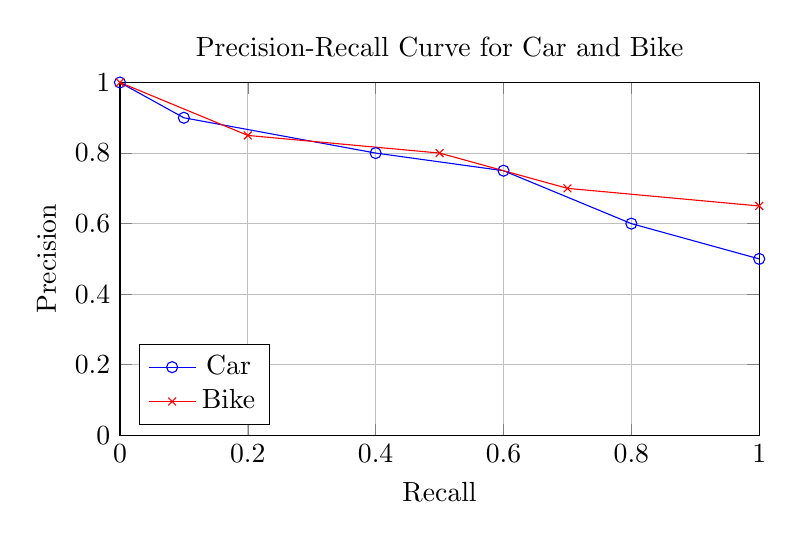
\begin{tikzpicture}
    \begin{axis}[
      xlabel={Recall},
      ylabel={Precision},
      title={Precision-Recall Curve for Car and Bike},
      legend pos=south west,
      grid=major,
      width=0.8\textwidth,
      height=0.5\textwidth,
      ymax=1.2,
      xmin=0, xmax=1, ymin=0, ymax=1
      ]
      \addplot[color=blue, mark=o] coordinates {
        (0, 1.0) (0.1, 0.9) (0.4, 0.8) (0.6, 0.75) (0.8, 0.6) (1.0, 0.5)
      };
      \addlegendentry{Car}
      \addplot[color=red, mark=x] coordinates {
        (0, 1.0) (0.2, 0.85) (0.5, 0.8) (0.7, 0.7) (1.0, 0.65)
      };
      \addlegendentry{Bike}
    \end{axis}
  \end{tikzpicture}
  \caption{Precision-Recall Curves for Car and Bike}
  \label{fig:pr_curve}
\end{figure}

\begin{enumerate}
  \item \textbf{Calculate Average Precision (AP)}

  For class \textit{Car}, we calculate the AP as:
  \[
  \text{AP}_{\text{Car}} = \frac{1}{6} \left(1.0 + 0.9 + 0.8 + 0.75 + 0.6 + 0.5\right) = 0.758
  \]

  For class \textit{Bike}, we calculate the AP as:
  \[
  \text{AP}_{\text{Bike}} = \frac{1}{5} \left(1.0 + 0.85 + 0.8 + 0.7 + 0.65\right) = 0.8
  \]

  \item \textbf{Compute Mean Average Precision (mAP)}

  Finally, we calculate the mAP as:
  \[
  \text{mAP} = \frac{1}{2} \left(0.758 + 0.8\right) = 0.779
  \]
\end{enumerate}

\paragraph{Using IoU in Object Detection}

In the context of object detection, Intersection over Union (IoU) is used to determine whether a predicted bounding box is a true positive or a false positive. The IoU is computed as follows:

\[
\text{IoU} = \frac{\text{Area of Overlap}}{\text{Area of Union}}
\]

A predicted bounding box is considered a true positive if its IoU with the ground truth bounding box exceeds a certain threshold (e.g., 0.5).

Example of mAP Calculation with IoU

Let's consider a set of predicted bounding boxes and their IoU with ground truth boxes for the class \textit{Car}:

\begin{itemize}
  \item Predicted Box 1: IoU = 0.7 (True Positive)
  \item Predicted Box 2: IoU = 0.4 (False Positive)
  \item Predicted Box 3: IoU = 0.6 (True Positive)
  \item Predicted Box 4: IoU = 0.3 (False Positive)
  \item Predicted Box 5: IoU = 0.8 (True Positive)
\end{itemize}

Using a threshold of 0.5 for IoU, we compute precision and recall at different confidence thresholds, plot the precision-recall curve, and calculate the AP as before.

\subsection{Object Tracking}

\paragraph{Motivation}
Object tracking involves following objects across frames in a video sequence. It is vital for applications like surveillance, autonomous driving, and human-computer interaction, where continuous monitoring of object movements is required.

\paragraph{Key Models}

\textbf{SORT (2016):}
\begin{itemize}
    \item \textbf{Mechanism:} Uses a combination of Kalman filtering and the Hungarian algorithm for data association.
    \item \textbf{Advantage:} High speed and simplicity, making it suitable for real-time applications.
\end{itemize}

\textbf{DeepSORT (2017):}
\begin{itemize}
    \item \textbf{Extension:} Enhances SORT by integrating a deep appearance descriptor.
    \item \textbf{Advantage:} Improved robustness against occlusions and re-identification.
\end{itemize}

\textbf{Siamese Networks (2016):}
\begin{itemize}
    \item \textbf{Mechanism:} Leverages a similarity learning approach to track objects.
    \item \textbf{Implementation:} Fully-Convolutional Siamese Networks learn a general similarity function offline, used to track objects in real-time.
\end{itemize}

\paragraph{QD-Track}

\paragraph{Architecture}
QD-Track (Query-Driven Tracking) is a multi-object tracking framework that leverages a query-based mechanism integrated with a transformer architecture. The core of QD-Track consists of a transformer encoder-decoder structure. The encoder processes the input video frames to extract feature representations, while the decoder utilizes a set of learnable queries to attend to these features and predict the locations and identities of the objects being tracked. Each query corresponds to a tracked object and is dynamically updated to maintain accurate associations across frames.

\paragraph{Key Insights}
The primary innovation of QD-Track is its use of a query mechanism for object tracking. This approach allows the model to dynamically manage and update object representations, which significantly enhances its ability to handle occlusions, appearance variations, and complex motion patterns. By leveraging the self-attention mechanism of transformers, QD-Track can capture long-range dependencies and contextual information, making it robust in challenging tracking scenarios.

\paragraph{Improvements Over Previous Works}
QD-Track introduces several improvements over traditional tracking methods:

\begin{itemize}
    \item \textbf{Query-Based Mechanism:} Traditional tracking methods often rely on manual association and heuristic rules for maintaining object identities. In contrast, QD-Track uses learnable queries that are updated iteratively, providing a more flexible and adaptive approach to track management.
    
    \item \textbf{Transformer Architecture:} The use of a transformer-based encoder-decoder structure allows QD-Track to effectively handle sequential data and capture complex relationships between objects over time. This results in improved tracking accuracy and robustness compared to methods that do not utilize such architectures.
    
    \item \textbf{Handling Occlusions and Appearance Variations:} The query-driven mechanism allows QD-Track to maintain consistent object identities even under occlusions or significant changes in appearance. This is a significant improvement over previous methods, which often struggle in such scenarios.
    
    \item \textbf{Efficiency:} QD-Track's architecture is designed to be computationally efficient, enabling real-time performance. This makes it suitable for practical applications such as autonomous driving, surveillance, and sports analytics, where real-time multi-object tracking is crucial.
\end{itemize}

\paragraph{Conclusion}
In summary, QD-Track represents a significant advancement in multi-object tracking by introducing a query-driven, transformer-based framework. Its ability to dynamically manage object representations, handle challenging tracking scenarios, and operate efficiently in real-time applications marks it as a notable improvement over traditional tracking methods.

\paragraph{Loss Functions and Metrics}
\begin{itemize}
    \item \textbf{Multi-Object Tracking Accuracy (MOTA):} Evaluates tracking performance by considering false positives, false negatives, and identity switches.
    \item \textbf{IDF1:} Measures the ratio of correctly identified detections to the average number of ground truth and computed detections.
\end{itemize}

\subsection{Segmentation}

Segmentation in computer vision refers to the process of partitioning an image into multiple segments, typically to locate objects and boundaries. There are various types of segmentation, including semantic segmentation, instance segmentation, and panoptic segmentation.

\subsubsection{Semantic Segmentation}

Semantic segmentation involves labeling each pixel in an image with a class from a predefined set. This task does not differentiate between different instances of the same class.

\paragraph{Key Models and Innovations}

\textbf{Fully Convolutional Networks (FCNs) (2015):}
\begin{itemize}
    \item \textbf{Architecture:} FCNs replace the fully connected layers in traditional CNNs with convolutional layers, allowing the network to output spatial maps.
    \item \textbf{Upsampling:} Uses deconvolutional (transposed convolution) layers to upsample feature maps back to the input image resolution.
    \item \textbf{Impact:} Set the groundwork for subsequent segmentation models by demonstrating end-to-end trainable networks for pixel-wise prediction.
\end{itemize}

\textbf{U-Net (2015):}
\begin{itemize}
    \item \textbf{Architecture:} U-Net features an encoder-decoder structure with skip connections between corresponding layers in the encoder and decoder.
    \item \textbf{Advantages:} The skip connections allow the model to capture both contextual and high-resolution information, making it particularly effective for biomedical image segmentation.
\end{itemize}

\textbf{DeepLab (2017):}
\begin{itemize}
    \item \textbf{Atrous Convolution:} DeepLab uses atrous (dilated) convolutions to capture multi-scale context without reducing spatial resolution.
    \item \textbf{Conditional Random Fields (CRFs):} Employs CRFs as a post-processing step to refine segmentation boundaries.
    \item \textbf{Variants:} DeepLabv2, DeepLabv3, and DeepLabv3+ introduced various improvements, including better multi-scale context aggregation and more efficient architectures.
\end{itemize}

\paragraph{Loss Functions and Metrics}

\textbf{Cross-Entropy Loss:}
\begin{itemize}
    \item Commonly used for semantic segmentation, applied to each pixel independently.
\end{itemize}

\textbf{Dice Loss:}
\begin{itemize}
    \item Measures the overlap between the predicted and ground truth segmentation masks, particularly useful for imbalanced datasets.
\end{itemize}

\textbf{Intersection over Union (IoU):}
\begin{itemize}
    \item Evaluates the overlap between predicted and ground truth regions, providing a standard metric for segmentation performance.
\end{itemize}

\subsubsection{Instance Segmentation}

Instance segmentation not only labels each pixel with a class but also differentiates between different instances of the same class.

\paragraph{Key Models and Innovations}

\textbf{Mask R-CNN (2017):}
\begin{itemize}
    \item \textbf{Extension of Faster R-CNN:} Mask R-CNN extends Faster R-CNN by adding a branch for predicting segmentation masks.
    \item \textbf{RoI Align:} Introduces RoI Align to improve mask accuracy by properly aligning the extracted features with the input.
    \item \textbf{Multi-task Loss:} Combines classification, bounding box regression, and mask prediction into a single framework.
\end{itemize}

\paragraph{RoI Pooling}

RoI Pooling is a process that converts the variable-sized regions of interest into a fixed-size feature map, which is necessary for downstream tasks such as classification and bounding box regression. It achieves this by dividing each RoI into a fixed number of bins and performing max pooling within each bin.

\paragraph{Mathematical Formulation}

Given an RoI, the RoI Pooling layer divides it into a grid of \( H \times W \) bins. For each bin, it selects the maximum value from the corresponding region of the input feature map. The result is a fixed-size feature map of \( H \times W \) for each RoI.

Let \((x_1, y_1)\) and \((x_2, y_2)\) be the coordinates of the top-left and bottom-right corners of an RoI, respectively. The width and height of the RoI are given by:

\[
w = x_2 - x_1 + 1, \quad h = y_2 - y_1 + 1
\]

Each bin size in the pooling layer is:

\[
w_{\text{bin}} = \frac{w}{W}, \quad h_{\text{bin}} = \frac{h}{H}
\]

For each bin, max pooling is applied:

\[
\text{pooled}(i, j) = \max_{(x, y) \in \text{bin}(i, j)} \text{feature}(x, y)
\]

where \( \text{bin}(i, j) \) represents the region in the input feature map corresponding to bin \( (i, j) \).

\paragraph{Limitations of RoI Pooling}

RoI Pooling introduces quantization errors due to the rounding of the coordinates of the bins, which can lead to misalignment between the RoIs and the extracted features. This can degrade the performance, especially in tasks requiring precise localization.

\paragraph{RoI Align}

RoI Align addresses the limitations of RoI Pooling by removing the quantization of the bin boundaries and using bilinear interpolation to compute the exact values of the input features at four regularly sampled locations in each bin. The final

 output is obtained by applying max or average pooling on these sampled values.

\paragraph{Mathematical Formulation}

RoI Align does not quantize the coordinates of RoI bins. Instead, it computes the coordinates of the sampling points and uses bilinear interpolation to get the feature values.

For an RoI, the size of each bin is computed as before, but the bin boundaries are not rounded. Each bin in RoI Align is subdivided into \( n \times n \) (e.g., \( 2 \times 2 \)) sub-bins, and the feature values at these sub-bin centers are computed using bilinear interpolation.

Let \( P \) be the feature map, and \((x, y)\) be a floating-point coordinate. The bilinear interpolation value \( P(x, y) \) is computed as:

\[
P(x, y) = \sum_{i=0}^{1} \sum_{j=0}^{1} w_{ij} P(\lfloor x \rfloor + i, \lfloor y \rfloor + j)
\]

where \( w_{ij} \) are the interpolation weights based on the distance from \((x, y)\) to its neighboring integer coordinates.

\paragraph{Importance of RoI Align}

RoI Align provides more accurate feature extraction by preserving the spatial alignment between the RoIs and the feature map. This leads to improved performance in object detection tasks, particularly in terms of localization accuracy.

\subparagraph{Comparison with RoI Pooling}

\begin{itemize}
    \item \textbf{Precision:} RoI Align provides higher precision by avoiding quantization errors, which are inherent in RoI Pooling.
    \item \textbf{Interpolation:} RoI Align uses bilinear interpolation to compute the feature values, while RoI Pooling uses max pooling, which can be less precise.
    \item \textbf{Performance:} Improved performance in tasks requiring precise localization, such as instance segmentation.
\end{itemize}

\textbf{PANet (2018):}
\begin{itemize}
    \item \textbf{Path Aggregation Network:} Enhances Mask R-CNN by improving information flow in the network, leading to better feature representation.
    \item \textbf{Advantages:} Demonstrates significant improvements in instance segmentation performance by leveraging precise localization and strong feature pyramids.
\end{itemize}

\paragraph{Mask2Former}

Mask2Former, introduced by Meta AI in 2022, is a versatile architecture capable of addressing various segmentation tasks, including panoptic, instance, and semantic segmentation. It builds upon the Meta architecture for mask classification and introduces several key innovations to improve performance and efficiency.

\paragraph{Architecture Overview}

Mask2Former employs a novel Transformer-based decoder that utilizes masked attention mechanisms instead of the standard cross-attention. This approach allows for better handling of high-resolution images and improves the convergence speed and performance of the model.

\begin{itemize}
    \item \textbf{Transformer Decoder with Masked Attention:} The core innovation in Mask2Former is the use of masked attention within the Transformer decoder. Masked attention ensures that each query attends to a specific region of the input, which helps in learning more accurate and localized features for segmentation.
    \item \textbf{Mask Classification:} Similar to the original Mask R-CNN, Mask2Former predicts a binary mask for each detected object. The mask classification head outputs a set of binary masks that are refined iteratively through the Transformer decoder.
    \item \textbf{Training Improvements:} Mask2Former introduces several training enhancements, such as better data augmentation techniques and loss functions, to improve the model's efficiency and accuracy.
\end{itemize}

\paragraph{Key Innovations and Contributions}

\begin{itemize}
    \item \textbf{Unified Segmentation Framework:} Mask2Former can handle panoptic, instance, and semantic segmentation tasks within a single framework. This unification simplifies the deployment of segmentation models in real-world applications.
    \item \textbf{Improved Convergence:} The masked attention mechanism in the Transformer decoder leads to faster convergence and better performance compared to traditional cross-attention mechanisms.
    \item \textbf{Efficient Handling of High-Resolution Images:} The architecture is designed to efficiently process high-resolution images, making it suitable for tasks requiring detailed and accurate segmentation, such as medical imaging and autonomous driving.
\end{itemize}

\paragraph{Performance and Applications}

Mask2Former has demonstrated state-of-the-art performance on various segmentation benchmarks, including COCO and ADE20K. Its ability to handle multiple segmentation tasks within a single model makes it a powerful tool for a wide range of applications, from autonomous driving to medical image analysis.

Mask2Former represents a significant advancement in the field of segmentation, offering a unified and efficient solution for panoptic, instance, and semantic segmentation tasks. Its innovative use of masked attention within the Transformer decoder sets a new standard for performance and versatility in segmentation models.

\paragraph{Detic}

\paragraph{Introduction and Context}
Detic, short for Detection Transformer, is an advanced object detection framework that builds upon the concept of transformers, initially designed for natural language processing (NLP), to improve object detection tasks in computer vision. The model leverages the self-attention mechanism of transformers to capture global dependencies and contextual information, which are crucial for accurately detecting and localizing objects in images.

\paragraph{Architecture}
Detic's architecture consists of several key components:
\begin{enumerate}
    \item \textbf{Backbone Network:} Typically a convolutional neural network (CNN) such as ResNet or a Vision Transformer (ViT) that extracts feature maps from the input images.
    \item \textbf{Transformer Encoder:} Processes the extracted feature maps to capture global dependencies and context. The encoder consists of multiple layers of self-attention and feed-forward networks.
    \item \textbf{Transformer Decoder:} Generates detection predictions by attending to the encoder's output and a set of learned object queries. Each query corresponds to a potential object in the image.
    \item \textbf{Prediction Heads:} Consist of fully connected layers that output the bounding boxes, class labels, and objectness scores for the detected objects.
\end{enumerate}

\paragraph{Key Innovations and Insights}
\begin{enumerate}
    \item \textbf{Self-Attention Mechanism:} By leveraging self-attention, Detic captures long-range dependencies and contextual information more effectively than traditional convolutional approaches. This leads to better detection performance, especially in complex scenes with multiple objects.
    \item \textbf{End-to-End Training:} Detic eliminates the need for heuristic components such as anchor generation and non-maximum suppression (NMS) by treating object detection as a direct set prediction problem. This simplifies the training process and allows for end-to-end optimization.
    \item \textbf{Object Queries:} The use of learned object queries enables the model to handle varying numbers of objects in images dynamically. Each query learns to attend to different parts of the image, effectively localizing and classifying objects.
\end{enumerate}

\paragraph{Technical Details}
\begin{enumerate}
    \item \textbf{Loss Function:} Detic uses a combination of classification and regression loss functions to train the model. The classification loss is typically a cross-entropy loss, while the regression loss for bounding box coordinates can be a smooth L1 loss or a generalized IoU loss.
    \item \textbf{Positional Encoding:} To incorporate spatial information, Detic adds positional encodings to the input features. This helps the model understand the relative positions of objects within the image.
    \item \textbf{Data Augmentation:} Detic employs various data augmentation techniques such as random cropping, resizing, flipping, and color jittering to improve the robustness and generalization of the model.
\end{enumerate}

\paragraph{Performance and Applications}
Detic has demonstrated state-of-the-art performance on various object detection benchmarks such as COCO and Pascal VOC. Its ability to capture global context and dependencies makes it particularly effective for detecting objects in challenging scenarios, including cluttered backgrounds and occlusions. Detic's applications span across autonomous driving, surveillance, medical imaging, and robotics, where accurate and reliable object detection is critical.

\paragraph{Limitations and Challenges}
\begin{enumerate}
    \item \textbf{Computational Complexity:} The self-attention mechanism in transformers has a quadratic complexity with respect to the input size, which can be computationally expensive for high-resolution images.
    \item \textbf{Data Requirements:} Detic, like other deep learning models, requires large amounts of annotated data for training. This can be a bottleneck in scenarios where labeled data is scarce.
    \item \textbf{Fine-Tuning:} While Detic performs well on standard benchmarks, fine-tuning it for specific applications or datasets may require careful hyperparameter tuning and domain adaptation techniques.
\end{enumerate}

Detic represents a significant advancement in the field of object detection by incorporating transformer-based architectures. Its ability to capture global context and dependencies has led to improved detection accuracy and robustness. As research in transformers for vision tasks continues to evolve, we can expect further enhancements in object detection models, making them more efficient and effective for real-world applications.


\subsubsection{Panoptic Segmentation}

Panoptic segmentation combines both semantic and instance segmentation, providing a complete scene understanding by labeling every pixel with either a semantic or instance label.

\paragraph{Key Models and Innovations}

\textbf{Panoptic FPN (2018):}
\begin{itemize}
    \item \textbf{Architecture:} Panoptic Feature Pyramid Networks (FPN) extend Feature Pyramid Networks to perform both semantic and instance segmentation.
    \item \textbf{Unified Model:} Uses separate heads for semantic and instance segmentation, combining the outputs to produce the final panoptic segmentation map.
\end{itemize}

\textbf{UPSNet (2019):}
\begin{itemize}
    \item \textbf{Unified Panoptic Segmentation Network:} UPSNet integrates a new panoptic head with a novel panoptic feature alignment module.
    \item \textbf{Advantages:} Achieves state-of-the-art performance with improved computational efficiency and segmentation accuracy.
\end{itemize}

\paragraph{Loss Functions and Metrics}

\textbf{Panoptic Quality (PQ):}
\begin{itemize}
    \item A comprehensive metric that evaluates both the segmentation quality (intersection over union) and recognition quality (detection score).
    \item Defined as \(PQ = \frac{\sum_{(p,g) \in TP} IoU(p, g)}{|TP| + \frac{1}{2}|FP| + \frac{1}{2}|FN|}\), where \(TP\), \(FP\), and \(FN\) are true positives, false positives, and false negatives, respectively.
\end{itemize}

\subsubsection{Loss Functions and Metrics for Segmentation}

\paragraph{Cross-Entropy Loss}
\begin{itemize}
    \item \textbf{Definition:} Computes the cross-entropy loss for each pixel, treating each pixel independently.
    \item \textbf{Formula:} Given a ground truth label \(y\) and a predicted probability \(p\), the loss for a single pixel is \(L_{CE} = -\sum y \log(p)\).
\end{itemize}

\paragraph{Dice Loss}
\begin{itemize}
    \item \textbf{Definition:} Measures the overlap between the predicted segmentation and the ground truth.
    \item \textbf{Formula:} \(L_{Dice} = 1 - \frac{2 |A \cap B|}{|A| + |B|}\), where \(A\) is the predicted set of pixels and \(B\) is the ground truth set.
    \item \textbf{Advantage:} Particularly effective for handling imbalanced datasets.
\end{itemize}

\paragraph{Intersection over Union (IoU)}
\begin{itemize}
    \item \textbf{Definition:} Evaluates the overlap between predicted and ground truth regions.
    \item \textbf{Formula:} \(IoU = \frac{|A \cap B|}{|A \cup B|}\), where \(A\) is the predicted set of pixels and \(B\) is the ground truth set.
    \item \textbf{Use:} Standard metric for segmentation performance, used in competitions like the COCO challenge.
\end{itemize}

IoU itself is not usually used as a loss function, however, \href{https://learnopencv.com/iou-loss-functions-object-detection/#ciou-complete-iou-loss}{GIoU, DIoU, and CIoU have been proposed as alternatives with a more smooth landscape.}

\subsection{Pose/Depth Estimation}

Pose and depth estimation are critical tasks in computer vision

 that involve understanding the spatial configuration of objects and their distances from the camera. These tasks have a wide range of applications, including robotics, augmented reality, and autonomous driving.

\subsubsection{Pose Estimation}

Pose estimation refers to the process of determining the position and orientation of an object or person within a given space. In human pose estimation, the goal is to localize key points on the human body, such as joints, to understand the pose of the person in the image or video.

\subparagraph{Key Concepts and Methods}

\textbf{Single-Person Pose Estimation:} This approach focuses on estimating the pose of a single individual in an image. Traditional methods often use part-based models, such as the Pictorial Structures Model, which represent the human body as a collection of connected parts. Modern approaches leverage deep learning techniques, particularly convolutional neural networks (CNNs), to directly predict the locations of key points.

\textbf{DeepPose (2014):} One of the first deep learning-based methods for human pose estimation, DeepPose uses a CNN to regress the positions of body joints from the input image. The objective is to minimize the Euclidean distance between the predicted and ground truth joint coordinates.

Let \( \hat{y}_i \) be the predicted coordinate of the \( i \)-th joint and \( y_i \) be the ground truth coordinate. The loss function used in DeepPose is:

\[
L = \sum_{i=1}^N \| \hat{y}_i - y_i \|^2
\]

where \( N \) is the number of joints.

\textbf{OpenPose (2016):} OpenPose introduces a bottom-up approach to multi-person pose estimation, where body parts are detected first and then assembled into full poses. This method uses Part Affinity Fields (PAFs) to associate body parts with individuals. The loss function consists of two terms: one for keypoint heatmaps and another for PAFs.

\[
L = \sum_{p=1}^P \sum_{i=1}^{N_p} \left( \| H_i^p - \hat{H}_i^p \|^2 + \| P_i^p - \hat{P}_i^p \|^2 \right)
\]

where \( P \) is the number of stages, \( N_p \) is the number of points in stage \( p \), \( H \) is the heatmap, and \( P \) is the PAF.

\textbf{PoseNet (2015):} PoseNet is designed for camera pose estimation, particularly for augmented reality applications. It uses a CNN to predict the 6-DoF (degrees of freedom) camera pose from a single RGB image. The loss function combines positional and rotational errors.

\[
L = \| \hat{t} - t \|^2 + \beta \| \hat{q} - q \|^2
\]

where \( \hat{t} \) and \( t \) are the predicted and ground truth translations, \( \hat{q} \) and \( q \) are the predicted and ground truth quaternions, and \( \beta \) is a scale factor to balance the two terms.

\textbf{HRNet (2019):} The High-Resolution Network (HRNet) maintains high-resolution representations throughout the network and combines them with multi-scale features. This architecture has set new benchmarks in human pose estimation by capturing detailed spatial information and preserving fine-grained features.

\paragraph{Challenges and Techniques}

Pose estimation faces several challenges, including occlusions, varying body shapes, and complex backgrounds. To address these challenges, researchers have developed various techniques:

\textbf{Multi-Scale Features:} Using features at different scales helps capture both global context and fine details, improving the accuracy of pose estimation in diverse scenarios.

\textbf{Data Augmentation:} Techniques such as rotation, scaling, and flipping are used to augment training data, helping the model generalize better to different poses and viewpoints.

\textbf{Heatmaps:} Many state-of-the-art methods predict heatmaps for each key point, where the intensity of the heatmap at each pixel indicates the likelihood of the key point being at that location. This approach provides spatial localization and helps refine predictions.

\subsubsection{Depth Estimation}

Depth estimation involves predicting the distance of each pixel in an image from the camera. This task is essential for 3D scene understanding and has applications in robotics, autonomous vehicles, and augmented reality.

\subparagraph{Key Concepts and Methods}

\textbf{Stereo Matching:} Traditional depth estimation methods often rely on stereo matching, which uses two images captured from slightly different viewpoints to triangulate the depth of objects. The disparity between corresponding points in the two images is used to compute depth.

\[
d = \frac{fB}{x_L - x_R}
\]

where \( d \) is the depth, \( f \) is the focal length, \( B \) is the baseline (distance between the two cameras), and \( x_L \) and \( x_R \) are the coordinates of the corresponding points in the left and right images.

\textbf{Depth from Monocular Images:} Recent advancements have enabled depth estimation from a single image, known as monocular depth estimation. This approach uses deep learning to infer depth by learning from large datasets of images with corresponding depth maps.

\textbf{Eigen et al. (2014):} This seminal work introduced a multi-scale deep network for monocular depth estimation. The network predicts coarse depth maps at a lower resolution and refines them using higher-resolution predictions, capturing both global context and local details.

\[
L = \frac{1}{n} \sum_{i} \left| \log d_i - \log d_i^* \right|
\]

where \( d_i \) is the predicted depth and \( d_i^* \) is the ground truth depth.

\textbf{DORN (2018):} The Deep Ordinal Regression Network (DORN) formulates depth estimation as an ordinal regression problem, predicting discrete depth levels instead of continuous values. This method improves depth estimation accuracy by leveraging ordinal relationships between depth levels.

\paragraph{SC-Depth}

SC-Depth (Self-Calibrating Depth) is a novel approach for monocular depth estimation that introduces self-calibrating mechanisms to enhance the accuracy and robustness of depth predictions. The primary innovation of SC-Depth lies in its ability to adaptively adjust its parameters and features based on the input image, thereby improving depth estimation performance in diverse and challenging scenarios.

\paragraph{Architecture}

The architecture of SC-Depth comprises three main components:

\begin{itemize}
    \item \textbf{Feature Extraction Backbone:} A convolutional neural network (CNN) backbone is used to extract rich, multi-scale features from the input image. Common choices for the backbone include ResNet or EfficientNet, which are known for their strong feature extraction capabilities.
    
    \item \textbf{Self-Calibrating Module:} This module is the core innovation of SC-Depth. It consists of a set of learnable parameters and dynamic filters that adjust based on the input image characteristics. The self-calibrating module processes the extracted features and refines them, ensuring that the depth estimation model is well-calibrated for each specific input.
    
    \item \textbf{Depth Prediction Head:} The refined features are fed into a depth prediction head, which typically includes upsampling layers and regression layers to produce the final depth map. The depth prediction head outputs a dense depth map where each pixel represents the estimated distance from the camera.
\end{itemize}

\paragraph{Key Insights}

SC-Depth introduces several key insights and improvements to monocular depth estimation:

\begin{itemize}
    \item \textbf{Adaptive Feature Calibration:} By incorporating a self-calibrating module, SC-Depth can adaptively fine-tune its parameters and features based on the specific input image. This adaptability allows the model to handle a wide range of lighting conditions, textures, and scene complexities.
    
    \item \textbf{Enhanced Robustness:} The ability to self-calibrate enables SC-Depth to maintain high performance even in challenging scenarios, such as low-light conditions, highly textured surfaces, and dynamic scenes. This robustness is a significant improvement over traditional depth estimation methods that may struggle in such conditions.
    
    \item \textbf{Improved Accuracy:} The dynamic adjustment of features ensures that the depth predictions are more accurate and consistent. SC-Depth leverages the flexibility of the self-calibrating module to correct potential errors and refine depth estimates in real-time.
\end{itemize}

\paragraph{Improvements Over Previous Works}

SC-Depth introduces several advancements over previous monocular depth estimation methods:

\begin{itemize}
    \item \textbf{Self-Calibrating Mechanism:} Unlike conventional models that use static parameters, SC-Depth's self-calibrating mechanism allows the model to dynamically adjust to different input conditions, leading to improved accuracy and robustness.
    
    \item \textbf{Handling Diverse Conditions:} SC-Depth excels in diverse and challenging environments, including varying lighting conditions and dynamic scenes. This versatility marks a significant improvement over previous methods that often require extensive training data for specific conditions.
    
    \item \textbf{Real-Time Performance:} Despite its sophisticated self-calibrating module, SC-Depth is designed to be computationally efficient, enabling real-time depth estimation. This efficiency makes it suitable for practical applications such as autonomous driving, robotics, and augmented reality.
\end{itemize}

\paragraph{Conclusion}

In conclusion, SC-Depth represents a significant step forward in monocular depth estimation by introducing a self-calibrating mechanism that enhances the model's adaptability, robustness, and accuracy. Its ability to dynamically adjust to varying input conditions and maintain real-time performance makes it a valuable addition to the field of depth estimation.

\paragraph{Challenges and Techniques}

Depth estimation presents several challenges, including varying lighting conditions, textureless surfaces, and dynamic scenes. To address these challenges, researchers use a variety of techniques:

\textbf{Loss Functions:} Designing effective loss functions, such as the BerHu loss and the Scale-Invariant Logarithmic Loss, helps improve depth estimation by penalizing large depth errors and emphasizing relative depth relationships.

\[
L_{\text{BerHu}} = \begin{cases} 
|x| & \text{if } |x| \leq c \\
\frac{x^2 + c^2}{2c} & \text{if } |x| > c 
\end{cases}
\]

\textbf{Data Augmentation:} Augmenting training data with synthetic depth maps, generated from computer graphics models or simulated environments, helps improve model robustness and generalization to real-world scenarios.

\textbf{Sensor Fusion:} Combining data from multiple sensors, such as RGB cameras, LiDAR, and depth sensors, provides complementary information and improves depth estimation accuracy, particularly in challenging environments.

\subsection{Image/Video Generation}

\subsubsection{Latent Diffusion Models for Image Generation}

Latent diffusion models (LDMs) are a class of generative models that have gained attention for their ability to produce high-quality images while avoiding some of the limitations associated with other generative models like variational autoencoders (VAEs). In this section, we provide an in-depth overview of the LDM architecture and discuss its advantages, including a comparison with VAEs.

\subsubsection{Latent Diffusion Model Architecture}

The core idea behind LDMs is to model the generation process as a diffusion process, starting from a simple noise distribution and progressively transforming it into a complex data distribution through a series of denoising steps. The diffusion process can be viewed as a continuous-time stochastic process, where the image is gradually corrupted by injecting noise at each time step. The reverse process, known as the denoising process, aims to learn a denoising function that can remove the injected noise and recover the original image.

The denoising function in LDMs is typically parameterized by a deep neural network, which is trained to minimize the difference between the denoised image and the ground truth image at each time step. The architecture of this network can vary, but it often includes components such as convolutional layers, residual connections, and normalization layers to facilitate efficient learning.

Once the denoising function is learned, it can be used to generate new images by sampling from the noise distribution and applying the denoising process in reverse. This is done by iteratively applying the learned denoising function to the noisy samples, progressively refining the generated images until they resemble samples from the target data distribution.

\subsubsection{Stable Diffusion}

A recent development in LDMs is the introduction of the stable diffusion framework, which improves the training and generation dynamics of LDMs by incorporating a stability-inducing regularization term into the training objective. This regularization term encourages the denoising function to be Lipschitz continuous, which helps prevent unstable behaviors during training and generation. As a result, stable diffusion models can generate even higher-quality images while maintaining stable training dynamics.

\subsubsection{Advantages of Latent Diffusion Models}

LDMs offer several advantages over other generative models, such as VAEs:

\textbf{Reconstruction Quality:} LDMs can generate high-quality images with sharp details, in contrast to VAEs, which often produce over-smoothed images due to the pixel-wise reconstruction loss term in their objective function.

\textbf{Posterior Collapse:} LDMs do not suffer from posterior collapse, a common issue in VAEs where the learned latent variables become less expressive and do not contribute significantly to the generative process.

\textbf{Stability and Training Dynamics:} LDMs benefit from a more direct and stable optimization problem, which results in improved training dynamics and stable convergence, leading to better image generation performance.

\textbf{Flexibility:} LDMs offer a flexible framework that can be adapted to a variety of tasks, such as conditional image generation and domain adaptation, by conditioning the denoising function on additional information.

In conclusion, latent diffusion models provide a powerful and flexible approach to image generation, with several advantages over alternative generative models like VAEs. The stable diffusion framework further enhances the performance and stability of LDMs, making them a promising choice for various image generation tasks.

\begin{figure}[h]
    \centering
    \includegraphics[scale=0.45]{./media/stablediff.jpeg}
    \caption{Stable Diffusion Architecture}
    \label{fig:stable_diff}
\end{figure}


\subsection{ 3D Reconstruction}

3D reconstruction is the process of capturing the shape and appearance of real objects and environments, creating a three-dimensional representation. This process is fundamental in applications such as computer graphics, virtual reality, autonomous driving, and medical imaging.

\subsubsection{Overview}

3D reconstruction techniques can be broadly categorized into passive and active methods:

\begin{itemize}
    \item \textbf{Passive Methods:} These methods rely on analyzing visual information from multiple images. Examples include Structure from Motion (SfM) and Multi-View Stereo (MVS).
    \item \textbf{Active Methods:} These methods use active sensors such as LiDAR or structured light to directly measure the 3D structure of the scene.
\end{itemize}

\subsubsection{Structure from Motion (SfM)}

Structure from Motion (SfM) is a passive technique that reconstructs 3D structure from a series of 2D images taken from different viewpoints. SfM simultaneously estimates the camera parameters and the 3D coordinates of points in the scene.

\paragraph{Key Steps}

\begin{enumerate}
    \item \textbf{Feature Detection and Matching:} Detect key points in each image and match them across images using descriptors like SIFT or ORB.
    \item \textbf{Initial Pose Estimation:} Use matched key points to estimate the relative camera poses (rotation and translation) using methods like the eight-point algorithm or PnP (Perspective-n-Point).
    \item \textbf{Bundle Adjustment:} Refine the camera poses and 3D points by minimizing the reprojection error, which is the difference between the observed and projected points.
\end{enumerate}

\paragraph{Mathematical Formulation}

Let \( x_{ij} \) be the projection of the 3D point \( X_j \) onto the image \( i \). The reprojection error \( e_{ij} \) is given by:

\[
e_{ij} = x_{ij} - \pi(K [R_i | t_i] X_j)
\]

where \( \pi \) is the projection function, \( K \) is the camera intrinsic matrix, and \( [R_i | t_i] \) are the rotation and translation matrices for the \( i \)-th camera.

The bundle adjustment minimizes the sum of squared reprojection errors:

\[
\min_{R_i, t_i, X_j} \sum_{i,j} \| e_{ij} \|^2
\]

\paragraph{Key Models and Intuitions}

\textbf{VisualSFM:}
\begin{itemize}
    \item VisualSFM is a popular tool that implements SfM using a graphical user interface (GUI) for ease of use.
    \item It integrates feature detection, matching, and bundle adjustment into a seamless workflow.
    \item The key intuition is to provide an accessible yet powerful solution for 3D reconstruction from multiple images.
\end{itemize}

\textbf{COLMAP:}
\begin{itemize}
    \item COLMAP is a general-purpose SfM and MVS pipeline with a command-line interface.
    \item It offers state-of-the-art algorithms for feature extraction, matching, and dense reconstruction.
    \item The intuition behind COLMAP is to offer flexibility and scalability for various 3D reconstruction tasks.
\end{itemize}

\subsubsection{Multi-View Stereo (MVS)}

Multi-View Stereo (MVS) builds on SfM by computing dense 3D point clouds from multiple images. MVS aims to reconstruct detailed 3D surfaces by finding correspondences across many images.

\paragraph{Key Techniques}

\begin{itemize}
    \item \textbf{Depth Map Estimation:} Compute depth maps for each image using stereo matching techniques.
    \item \textbf{Fusion:} Combine depth maps into a consistent 3D model by merging and filtering the points.
\end{itemize}

\paragraph{Mathematical Formulation}

The depth \( d \) of a point can be estimated using the disparity \( \delta \) between corresponding points in stereo images:

\[
d = \frac{B f}{\delta}
\]

where \( B \) is the baseline distance between the cameras, and \( f \) is the focal length.

\paragraph{Key Models and Intuitions}

\textbf{PMVS (Patch-based Multi-View Stereo):}
\begin{itemize}
    \item PMVS reconstructs surfaces by expanding small image patches across views.
    \item The intuition is to achieve robust and accurate dense reconstruction by aggregating information from multiple images.
\end{itemize}

\textbf{OpenMVS:}
\begin{itemize}
    \item OpenMVS is an open-source library that provides tools for dense 3D reconstruction.
    \item It integrates depth map estimation, fusion, and surface reconstruction into a complete pipeline.
    \item The key intuition is to offer an accessible and extensible solution for high-quality 3D reconstruction.
\end{itemize}

\subsubsection{Active Methods}

Active methods use sensors to directly capture depth information. These methods include LiDAR, structured light, and time-of-flight cameras.

\paragraph{LiDAR}

LiDAR (Light Detection and Ranging) uses laser pulses to measure distances to objects. By scanning the environment, LiDAR generates a dense 3D point cloud.

\[
d = \frac{ct}{2}
\]

where \( d \) is the distance, \( c \) is the speed of light, and \( t \) is the time taken for the laser pulse to return.

\paragraph{Structured Light}

Structured light projects a known pattern onto the scene and captures the deformation of the pattern to compute depth. The depth \( z \) is calculated using triangulation.

\[
z = \frac{B f}{d}
\]

where \( B \) is the baseline distance between the projector and camera, \( f \) is the focal length, and \( d \) is the disparity.

\paragraph{Time-of-Flight (ToF) Cameras}

ToF cameras measure the time it takes for light to travel to an object and back to compute depth. This method provides real-time depth information.

\subsubsection{Challenges}

\begin{itemize}
    \item \textbf{Occlusions:} Objects may be partially or fully occluded in some views, making it challenging to reconstruct the complete 3D shape.
    \item \textbf{Textureless Surfaces:} Surfaces with little texture provide few features for matching.
    \item \textbf{Computational Complexity:} Dense 

3D reconstruction requires significant computational resources.
\end{itemize}

\subsubsection{NeRF}

Neural Radiance Fields (NeRF) are a class of models designed for 3D scene representation and rendering. NeRF models use a fully connected deep neural network to represent a continuous volumetric scene function, which maps 3D coordinates and viewing directions to RGB color and volume density.

\paragraph{NeRF Architecture}

The core of NeRF is a neural network that takes in a 3D position and a viewing direction as input and outputs the color and density at that position. The network is trained on a set of 2D images of the scene along with their camera parameters. During training, the network learns to approximate the volumetric scene function that best fits the observed images.

The rendering process involves casting rays through the scene, accumulating color and density values along each ray using volumetric rendering techniques. This allows NeRF to synthesize novel views of the scene from arbitrary camera positions.

\paragraph{Applications of NeRF}

NeRF has been successfully applied to various tasks, including:
\begin{itemize}
    \item Novel view synthesis
    \item 3D reconstruction
    \item Virtual reality and augmented reality applications
\end{itemize}

\paragraph{Advantages of NeRF}

\textbf{High-Quality Rendering:} NeRF can produce photorealistic images with fine details and complex lighting effects.

\textbf{Continuous Representation:} Unlike voxel grids or mesh-based methods, NeRF provides a continuous representation of the scene, allowing for smooth interpolation between views.

\textbf{Flexibility:} NeRF can be trained on different types of scenes, from synthetic to real-world environments, and can generalize to novel views not seen during training.

\subsubsection{Gaussian Splatting}

Gaussian splatting is a technique used in 3D reconstruction and neural scene representation. It involves representing a 3D scene using Gaussian functions to model the geometry and appearance of objects within the scene. This method offers several advantages, including efficient rendering and the ability to capture fine details compared to NeRF.

\paragraph{Overview}

In Gaussian splatting, a 3D scene is represented by a collection of Gaussians, each defined by parameters such as mean, covariance, and color. These Gaussians can be used to approximate the appearance of the scene when projected onto a 2D image plane.

\paragraph{Mathematical Formulation}

Each Gaussian in the 3D scene can be defined by its mean \( \mu \), covariance matrix \( \Sigma \), and color \( c \). The projection of a Gaussian onto a 2D image plane results in an elliptical shape with its own mean and covariance, influenced by the camera's position and orientation.

The intensity \( I \) of a pixel \( (x, y) \) in the image can be calculated by summing the contributions of all Gaussians:

\[
I(x, y) = \sum_{i} w_i \exp \left( -\frac{1}{2} (p - \mu_i)^T \Sigma_i^{-1} (p - \mu_i) \right)
\]

where \( w_i \) is the weight of the \(i\)-th Gaussian, \( \mu_i \) and \( \Sigma_i \) are the mean and covariance of the \(i\)-th Gaussian, and \( p \) is the position of the pixel.

\paragraph{Rendering Process}

The rendering process involves projecting each 3D Gaussian onto the image plane and accumulating their contributions to compute the final pixel intensities. This can be done efficiently using GPU acceleration, making Gaussian splatting suitable for real-time applications.

\paragraph{Advantages over NeRF}

\textbf{Rendering Efficiency:} Gaussian splatting can be rendered efficiently using GPU acceleration, enabling real-time performance, whereas NeRF is computationally intensive and slower to render.

\textbf{Detail Preservation:} Gaussian splatting captures fine details of the 3D scene, providing high-quality visual representations similar to NeRF but with potentially faster rendering times.

\textbf{Ease of Implementation:} Gaussian splatting is often simpler to implement and can achieve comparable visual quality with less computational overhead.

\paragraph{Similarities to NeRF}

\textbf{Scene Representation:} Both NeRF and Gaussian splatting represent 3D scenes and are used for novel view synthesis and 3D reconstruction.

\textbf{Applications:} Both techniques are applied in virtual reality, augmented reality, and high-quality rendering tasks.

\paragraph{Differences from NeRF}

\textbf{Representation Method:} NeRF uses a neural network to model the scene as a continuous volumetric function, while Gaussian splatting uses a collection of discrete Gaussian functions.

\textbf{Rendering Approach:} NeRF performs volumetric rendering by casting rays and accumulating color and density along each ray. Gaussian splatting projects Gaussians onto the image plane and accumulates their contributions.

\textbf{Computational Requirements:} NeRF is more computationally intensive and requires longer training times, whereas Gaussian splatting can achieve efficient rendering with GPU acceleration.

\paragraph{Applications}

Gaussian splatting has various applications, including:
\begin{itemize}
    \item \textbf{3D Scene Reconstruction:} Creating detailed and accurate 3D models of real-world scenes.
    \item \textbf{Neural Rendering:} Generating photorealistic images from 3D models.
    \item \textbf{Virtual Reality and Augmented Reality:} Enhancing the realism and immersion of virtual environments.
\end{itemize}

\paragraph{Advantages}

\begin{itemize}
    \item \textbf{Efficiency:} Gaussian splatting can be efficiently implemented using GPU acceleration, enabling real-time rendering.
    \item \textbf{Detail Preservation:} The technique captures fine details of the 3D scene, providing high-quality visual representations.
    \item \textbf{Flexibility:} Gaussian splatting can be combined with other neural rendering techniques to enhance performance and visual quality.
\end{itemize}


\subsection{Optical Flow and Motion Estimation}

Optical flow and motion estimation are essential techniques in computer vision for understanding and analyzing the motion of objects within a sequence of images or a video. These techniques have applications in areas such as video compression, object tracking, and autonomous driving.

\subsubsection{Optical Flow}

Optical flow refers to the apparent motion of objects between consecutive frames of a video, caused by the relative motion between the observer and the scene. The goal of optical flow estimation is to compute a vector field where each vector represents the displacement of a pixel from one frame to the next.

\paragraph{Mathematical Formulation}

Let \( I(x, y, t) \) be the intensity of the image at pixel \((x, y)\) and time \( t \). Assuming that the intensity of a point remains constant over time, the optical flow constraint equation can be derived as:

\[
I(x, y, t) = I(x + u, y + v, t + 1)
\]

where \( (u, v) \) represents the optical flow vector at pixel \((x, y)\).

Using a first-order Taylor series expansion, this equation can be approximated as:

\[
I(x + u, y + v, t + 1) \approx I(x, y, t) + \frac{\partial I}{\partial x} u + \frac{\partial I}{\partial y} v + \frac{\partial I}{\partial t}
\]

By subtracting \( I(x, y, t) \) from both sides, we get:

\[
\frac{\partial I}{\partial x} u + \frac{\partial I}{\partial y} v + \frac{\partial I}{\partial t} = 0
\]

This can be written in a compact form as:

\[
\nabla I \cdot \mathbf{v} + I_t = 0
\]

where \( \nabla I \) is the spatial gradient of the image, \( \mathbf{v} = (u, v) \) is the optical flow vector, and \( I_t \) is the temporal gradient.

\paragraph{Key Methods}

\textbf{Lucas-Kanade Method:}
\begin{itemize}
    \item Assumes that the flow is constant within a small neighborhood around each pixel.
    \item Solves for the flow vector \( \mathbf{v} \) using a least squares approach.
    \item The system of equations for a pixel and its neighbors can be written as:
    \[
    A \mathbf{v} = \mathbf{b}
    \]
    where \( A \) is a matrix of image gradients and \( \mathbf{b} \) is a vector of temporal gradients.
\end{itemize}

\textbf{Horn-Schunck Method:}
\begin{itemize}
    \item Assumes that the flow is smooth over the entire image.
    \item Introduces a global smoothness term to the optical flow constraint equation.
    \item The energy function to be minimized is:
    \[
    E = \int \int \left( (\nabla I \cdot \mathbf{v} + I_t)^2 + \alpha^2 (\|\nabla u\|^2 + \|\nabla v\|^2) \right) \, dx \, dy
    \]
    where \( \alpha \) is a regularization parameter.
\end{itemize}

\subsubsection{Motion Estimation}

Motion estimation is the process of determining the motion vectors that describe the transformation from one image to another in a sequence. It is closely related to optical flow but can involve more complex transformations, such as rotations and scalings.

\paragraph{Block Matching}

Block matching is a common technique used for motion estimation in video compression. The image is divided into blocks, and for each block in the current frame, the most similar block in the reference frame is found. The displacement between these blocks is the motion vector.

\textbf{Sum of Absolute Differences (SAD):}
\begin{itemize}
    \item Measures the similarity between blocks by calculating the sum of absolute differences of pixel intensities.
    \item For a block \( B \) in the current frame and a candidate block \( B' \) in the reference frame, the SAD is given by:
    \[
    \text{SAD} = \sum_{i, j} |I(i, j) - I'(i + u, j + v)|
    \]
    where \( (u, v) \) is the displacement vector.
\end{itemize}

\textbf{Normalized Cross-Correlation (NCC):}
\begin{itemize}
    \item Measures the similarity between blocks using cross-correlation.
    \item For blocks \( B \) and \( B' \), the NCC is given by:
    \[
    \text{NCC} = \frac{\sum_{i, j} (I(i, j) - \bar{I})(I'(i + u, j + v) - \bar{I'})}{\sqrt{\sum_{i, j} (I(i, j) - \bar{I})^2 \sum_{i, j} (I'(i + u, j + v) - \bar{I'})^2}}
    \]
    where \( \bar{I} \) and \( \bar{I'} \) are the mean intensities of the blocks \( B \) and \( B' \).
\end{itemize}

\subsubsection{Applications}

Optical flow and motion estimation are used in various applications, including:

\begin{itemize}
    \item \textbf{Video Compression:} Efficiently encoding motion between frames to reduce data size.
    \item \textbf{Object Tracking:} Following the movement of objects across frames in a video.
    \item \textbf{Autonomous Driving:} Understanding the motion of vehicles and pedestrians for navigation and collision avoidance.
    \item \textbf{Stabilization:} Correcting camera shake and jitter in videos.
\end{itemize}

\subsubsection{Challenges}

\begin{itemize}
    \item \textbf{Occlusions:} Parts of the scene may be occluded in some frames, making it difficult to track motion.
    \item \textbf{Lighting Changes:} Variations in lighting can affect the accuracy of motion estimation.
    \item \textbf{Large Motions:} Handling large displacements between frames can be challenging.
\end{itemize}

\subsection{Vision Transformers (ViT) and Successors}

The Vision Transformer (ViT) architecture represents a significant innovation in computer vision by applying the transformer model, originally designed for natural language processing (NLP), to image data. ViTs and their successors have shown that self-attention mechanisms can be highly effective for image classification and other vision tasks.

\subsubsection{Vision Transformer (ViT)}

\paragraph{Introduction}

The Vision Transformer (ViT) introduced in the paper "An Image is Worth 16x16 Words: Transformers for Image Recognition at Scale." ViT adapts the transformer architecture to handle image data by treating image patches as tokens, similar to words in text.

\paragraph{Architecture Overview}

\paragraph{Patch Embedding}

ViT processes an image by dividing it into fixed-size, non-overlapping patches. Each patch is then flattened and linearly projected into an embedding vector. This step converts the image into a sequence of patch embeddings, akin to token embeddings in NLP.

\[
\text{Patch Embedding} = \text{Linear}(\text{Flatten}(x))
\]

Given an input image \(x \in \mathbb{R}^{H \times W \times C}\), it is divided into patches of size \(P \times P\), resulting in \(\frac{HW}{P^2}\) patches. Each patch is flattened into a vector and projected linearly to a fixed size \(D\).

\paragraph{Position Embedding}

To retain spatial information, learnable position embeddings are added to the patch embeddings. This allows the model to incorporate the order and relative positions of patches within the image.

\[
z_0 = [x_{class}; x_p^1 E; x_p^2 E; \dots; x_p^N E] + E_{pos}
\]

where \(x_{class}\) is a learnable class token prepended to the sequence, \(E\) is the patch embedding projection, and \(E_{pos}\) is the position embedding.

\paragraph{Transformer Encoder}

The sequence of embedded patches is passed through a stack of transformer encoder layers. Each encoder layer comprises multi-head self-attention (MHSA) and a feedforward neural network (FFN), with residual connections and layer normalization.

\paragraph{Multi-Head Self-Attention (MHSA)}

MHSA allows the model to capture relationships between different patches by computing attention scores for each patch with respect to all other patches. The self-attention mechanism calculates these scores using the query, key, and value matrices derived from the input embeddings.

\[
\text{Attention}(Q, K, V) = \text{softmax} \left( \frac{QK^T}{\sqrt{d_k}} \right) V
\]

\paragraph{Feedforward Neural Network (FFN)}

The FFN consists of two linear layers with a ReLU or GELU activation in between. It is applied independently to each token in the sequence.

\[
\text{FFN}(x) = W_2 \cdot \text{GELU}(W_1 \cdot x + b_1) + b_2
\]

\paragraph{Classification Head}

After passing through the transformer encoder layers, the output corresponding to the class token is fed into a classification head, typically a linear layer, to produce the final class probabilities.

\[
\text{Class Probabilities} = \text{softmax}(W \cdot z_L^0)
\]

where \(z_L^0\) is the output embedding of the class token from the last transformer encoder layer.

\paragraph{Training and Performance}

ViT models are pre-trained on large datasets (e.g., JFT-300M) and then fine-tuned on smaller datasets (e.g., ImageNet). They have demonstrated competitive performance with traditional CNN-based models, particularly when large-scale data is available for pre-training.

\paragraph{Advantages and Challenges}

\begin{itemize}
    \item \textbf{Advantages:} ViT leverages self-attention to capture long-range dependencies and global context effectively, leading to strong performance in image classification tasks.
    \item \textbf{Challenges:} ViT requires large amounts of data for pre-training to achieve competitive performance and has higher computational complexity for long sequences of patches.
\end{itemize}

\begin{figure}[h]
    \centering
    \includegraphics[width=0.7\textwidth]{./media/vit.png}
    \caption{ViT Architecture}
    \label{fig:vit}
\end{figure}

\subsubsection{Successors of Vision Transformer (ViT)}

\paragraph{Swin Transformer (2021)}

\paragraph{Introduction}

The Swin Transformer introduced in the paper "Swin Transformer: Hierarchical Vision Transformer using Shifted Windows," aims to address the computational inefficiencies of ViT by introducing a hierarchical architecture and local self-attention mechanisms.

\paragraph{Architecture Overview}

\paragraph{Shifted Window Self-Attention}

\textbf{Window-Based Self-Attention:} The Swin Transformer divides the image into non-overlapping windows and computes self-attention within each window. This reduces the computational complexity compared to global self-attention.

\[
\text{Attention}(Q, K, V) = \text{softmax} \left( \frac{QK^T}{\sqrt{d_k}} + B \right) V
\]

where \(B\) is a relative position bias that encodes the spatial relationship between patches within a window.

\paragraph{Shifted Window Partitioning}

To enable cross-window interactions, the windows are shifted by a fixed offset between consecutive layers. This shifting mechanism ensures that each patch can attend to patches from neighboring windows, enhancing the model's ability to capture global context.

\paragraph{Hierarchical Structure}

The Swin Transformer employs a hierarchical structure with multiple stages, where the patch size is doubled, and the number of patches is reduced by a factor of 4 at each stage. This design allows the model to process high-resolution images efficiently.

\paragraph{Transformer Blocks}

Each stage consists of multiple transformer blocks, each containing a shifted window-based self-attention layer followed by a feedforward network (FFN).

\paragraph{Advantages and Performance}

\begin{itemize}
    \item \textbf{Advantages:} Swin Transformer reduces the computational complexity of self-attention and improves the model's ability to capture hierarchical features, leading to state-of-the-art performance on image classification, object detection, and segmentation tasks.
    \item \textbf{Performance:} Swin Transformer achieves better accuracy and efficiency compared to ViT and CNN-based models on various benchmarks.
\end{itemize}

\begin{figure}[h]
    \centering
    \includegraphics[width=0.7\textwidth]{./media/swin_vit.png}
    \caption{Swin ViT Architecture}
    \label{fig:vit}
\end{figure}

\paragraph{Other Relevant Successors}

\paragraph{DeiT (2021)}

The Data-efficient Image Transformer (DeiT) improves the data efficiency of ViTs, enabling competitive performance with smaller datasets. DeiT uses a teacher-student training strategy and knowledge distillation to enhance the learning process.

\paragraph{Segmenter (2021)}

Segmenter adapts ViTs for semantic segmentation tasks. It uses a transformer encoder to process image patches and a lightweight decoder to generate segmentation masks, demonstrating strong performance on benchmarks like ADE20K.

\paragraph{MViT (2021)}

The Multiscale Vision Transformer (MViT) introduces multiscale feature hierarchies within the transformer framework, enabling efficient processing of high-resolution images. MViT shows improvements in both accuracy and computational efficiency for tasks like image classification and object detection.


\subsection{Foundation Models in Computer Vision}

Foundation models have revolutionized computer vision tasks such as image classification, object detection, and image segmentation. These models, initially limited to language tasks, have begun transforming industries like autonomous driving, medical imaging, and robotics by providing unprecedented visual understanding.

\subsubsection{What is a Foundation Model?}

A foundation model is a pre-trained deep neural network that serves as the backbone for various downstream tasks such as object classification, object detection, and image segmentation. Trained on massive, diverse datasets, these models capture visual features universal to many domains. This approach leverages neural networks’ powerful representational learning capabilities to generalize well across tasks.

\begin{figure}[h]
    \centering
    \includegraphics[scale=0.3]{./media/cv_foundational_models.png}
    \caption{CV Foundation Models}
    \label{fig:foundation_cv}
\end{figure}

\subsubsection{Embedding Extractors}

Embedding extractors are a subset of foundation models that transform raw input data, like images, into compact vector representations, known as embeddings. These embeddings capture meaningful features from the input data and are crucial for transferring knowledge from a pre-trained model to a specific task.

\paragraph{CLIP (OpenAI, 2021)}

\begin{itemize}
    \item \textbf{Inputs:} Images and Text.
    \item \textbf{Outputs:} Dense vector representations (embeddings) for both the input image and text that preserve semantic similarity.
    \item \textbf{Description:} CLIP (Contrastive Language-Image Pre-training) is a series of multimodal image and text encoders that understand and interpret images in the context of natural language.
\end{itemize}

\paragraph{DINOv2 (Meta AI, 2023)}

\begin{itemize}
    \item \textbf{Inputs:} Images.
    \item \textbf{Outputs:} Dense semantic vector representations for the input image.
    \item \textbf{Description:} DINOv2 focuses on the vision domain with a novel self-supervised training setup designed to maximize performance on downstream vision tasks.
\end{itemize}

\paragraph{ImageBind (Meta AI, 2023)}

\begin{itemize}
    \item \textbf{Inputs:} Images, Text, Audio, Depth Maps, Thermal Image Maps, and Inertial Measurement Units.
    \item \textbf{Outputs:} Dense semantic vector representations.
    \item \textbf{Description:} ImageBind is a multimodal encoder that supports various mediums, improving image and text encoding support.
\end{itemize}

\subsubsection{Zero-Shot Models}

Zero-shot models are pre-trained neural networks that aim to perform tasks directly on unseen data without requiring additional training. These models are particularly useful in scenarios with many object categories and little or no labeled data.

\paragraph{Segment Anything Model (Meta AI, 2023)}

\begin{itemize}
    \item \textbf{Inputs:} Images and Point Prompts.
    \item \textbf{Outputs:} Instance segmentations of objects at the given point.
    \item \textbf{Description:} The Segment Anything Model (SAM) segments any object in an image or video with high quality and efficiency, generalizing zero-shot to unfamiliar objects and images.
\end{itemize}

\paragraph{OWL-ViT (Google Research, 2022)}

\begin{itemize}
    \item \textbf{Inputs:} Images and a Text Query.
    \item \textbf{Outputs:} Open-Set Object Detection.
    \item \textbf{Description:} OWL-ViT is an open-set object detector that can find object bounding boxes matching a text query, performing zero-shot object detection.
\end{itemize}

\subsubsection{State-of-the-Art Architectures}

State-of-the-art architectures have proven their effectiveness in industrial object classification, detection, and segmentation tasks. Unlike foundation models, these architectures require bespoke training on a given task and labeled dataset.

\paragraph{YOLO-NAS (Deci.ai, 2023)}

\begin{itemize}
    \item \textbf{Inputs:} Images.
    \item \textbf{Outputs:} Object Detection.
    \item \textbf{Description:} YOLO-NAS (You Only Look Once — Neural Architecture Search) provides state-of-the-art real-time object detection capabilities.
\end{itemize}

\paragraph{Mask2Former (Meta AI, 2022)}

\begin{itemize}
    \item \textbf{Inputs:} Images.
    \item \textbf{Outputs:} Panoptic, Instance, and Semantic Segmentation.
    \item \textbf{Description:} Mask2Former introduces a new Transformer decoder using masked attention, improving convergence and performance for segmentation tasks.
\end{itemize}

\paragraph{DETR (Meta AI, 2020)}

\begin{itemize}
    \item \textbf{Inputs:} Images.
    \item \textbf{Outputs:} Object Detection.
    \item \textbf{Description:} DETR (DEtection TRansformer) views object detection as a direct set prediction problem, streamlining the detection pipeline.
\end{itemize}

TODO: Learn more about this DETR model. X-coder

Flamingo? BLIP-2 MPLUG-OWN. Otter. Kosmos-2. DetGPT. GPT4RoI

\paragraph{ConvNeXt (Meta AI, 2022)}

\begin{itemize}
    \item \textbf{Inputs:} Images.
    \item \textbf{Outputs:} Classification, Object Detection, and Segmentation.
    \item \textbf{Description:} ConvNeXt co-designs self-supervised learning techniques and architectural improvements to enhance the performance of ConvNets on various recognition benchmarks.
\end{itemize}

\subsection{Self-Supervised \& Weakly Supervised}

Self-supervised, weakly supervised, and unsupervised learning are crucial paradigms in machine learning, enabling models to learn from unlabeled or partially labeled data. These approaches are particularly valuable in scenarios where labeled data is scarce or expensive to obtain. This section covers key concepts, methods, and notable models, focusing on their applications in computer vision.

\subsubsection{Overview of Self-Supervised Learning}

Self-supervised learning leverages the inherent structure of data to create surrogate labels for training. This involves designing pretext tasks, which are auxiliary tasks that enable the model to learn useful representations without explicit human annotations.

\paragraph{Common Pretext Tasks}

\begin{itemize}
    \item \textbf{Colorization:} Predicting the color channels of an image given the grayscale version.
    \item \textbf{Jigsaw Puzzles:} Rearranging shuffled patches of an image back to their original positions.
    \item \textbf{Rotation Prediction:} Determining the rotation angle applied to an image.
    \item \textbf{Contrastive Learning:} Learning representations by distinguishing between similar and dissimilar image pairs.
\end{itemize}

\subsection{Contrastive Learning}

Contrastive learning is a self-supervised learning technique that learns useful representations by comparing similar and dissimilar pairs of data points. The key idea is to bring similar (positive) pairs closer in the representation space and push dissimilar (negative) pairs apart.

\subsubsection{Architecture}

A typical architecture for contrastive learning includes an encoder network, which can be a convolutional neural network (CNN) or a transformer, followed by a projection head that maps the encoded features to a lower-dimensional space suitable for computing similarities.

\begin{itemize}
    \item \textbf{Encoder Network:} Extracts features from the input images.
    \item \textbf{Projection Head:} Maps the features to a space where contrastive loss is applied.
\end{itemize}

For example, in SimCLR (Simple Framework for Contrastive Learning of Visual Representations), the architecture consists of a ResNet encoder followed by a multi-layer perceptron (MLP) projection head.

\subsubsection{Mathematical Formulation}

The core of contrastive learning is the contrastive loss function, which aims to minimize the distance between positive pairs and maximize the distance between negative pairs. The most commonly used contrastive loss is the InfoNCE (Information Noise Contrastive Estimation) loss.

Given a batch of $N$ images, we generate $2N$ augmented views (two for each image). Let $z_i$ and $z_j$ be the representations of a positive pair, and $z_k$ be the representation of a negative sample. The contrastive loss for a positive pair $(i, j)$ is defined as:

\[
\ell_{i,j} = -\log \frac{\exp(\text{sim}(z_i, z_j) / \tau)}{\sum_{k=1}^{2N} \mathbb{1}_{[k \neq i]} \exp(\text{sim}(z_i, z_k) / \tau)}
\]

where $\text{sim}(z_i, z_j)$ denotes the cosine similarity between $z_i$ and $z_j$, and $\tau$ is a temperature parameter.

The total loss is computed by averaging over all positive pairs in the batch:

\[
L = \frac{1}{2N} \sum_{k=1}^{N} \left( \ell_{2k-1, 2k} + \ell_{2k, 2k-1} \right)
\]

\subsubsection{Intuition Behind Contrastive Learning}

The intuition behind contrastive learning is to learn a representation space where similar inputs (positive pairs) are closer together and dissimilar inputs (negative pairs) are farther apart. This is achieved by contrasting the positive pairs against a large number of negative pairs, effectively teaching the model to discern subtle differences and similarities in the data.

\subsubsection{Key Approaches}

Several key approaches in contrastive learning have been proposed:

\begin{itemize}
    \item \textbf{SimCLR (Simple Framework for Contrastive Learning of Visual Representations):} Uses extensive data augmentation and a simple contrastive loss to learn visual representations without labels.
    \item \textbf{MoCo (Momentum Contrast):} Introduces a memory bank to store a large number of negative samples efficiently.
    \item \textbf{BYOL (Bootstrap Your Own Latent):} Eliminates the need for negative pairs by using a target network that slowly updates with the moving average of the online network.
\end{itemize}

\subsubsection{Applications}

Contrastive learning has shown great promise in various computer vision tasks, including:

\begin{itemize}
    \item \textbf{Image Classification:} Pre-trained models using contrastive learning achieve competitive performance on standard classification benchmarks.
    \item \textbf{Object Detection:} Learned representations can be fine-tuned for object detection tasks.
    \item \textbf{Image Segmentation:} Contrastive learning helps in learning representations useful for pixel-level segmentation tasks.
\end{itemize}

Contrastive learning leverages the abundance of unlabeled data, making it a powerful tool in self-supervised learning for computer vision. The representations learned through contrastive learning are general and can be effectively transferred to various downstream tasks, significantly reducing the need for labeled data.

\subsubsection{Masked Autoencoders (MAEs)}

Masked Autoencoders (MAEs) are significant in self-supervised learning, especially for vision tasks. MAEs are designed to reconstruct missing parts of their input, typically images, by learning a robust latent representation.

\paragraph{Concept and Architecture}

\begin{itemize}
    \item \textbf{Input Masking:} Randomly mask a significant portion of the input image.
    \item \textbf{Encoder:} Processes the partially visible image to produce a latent representation.
    \item \textbf{Decoder:} Attempts to reconstruct the original image from the latent representation.
\end{itemize}

\paragraph{Training Objective}

The objective of MAEs is to minimize the reconstruction loss, measuring the difference between the reconstructed image and the original image. Common loss functions include Mean Squared Error (MSE) and L1 loss.

\paragraph{Advantages and Applications}

\begin{itemize}
    \item \textbf{Efficient Learning:} Learn robust feature representations from unlabeled data.
    \item \textbf{Transfer Learning:} Pre-trained MAEs can be fine-tuned for various downstream tasks such as classification, detection, and segmentation.
    \item \textbf{Better Generalization:} Helps models generalize better to new tasks and datasets.
\end{itemize}

\subsubsection{Weakly Supervised Learning}

Weakly supervised learning involves training models using weak labels, which are often cheaper to obtain but less precise than full labels. These include noisy, incomplete, or inexact labels.

\paragraph{Common Approaches}

\begin{itemize}
    \item \textbf{Multiple Instance Learning (MIL):} Learns from labeled bags of instances, where only the bag label is known.
    \item \textbf{Label Propagation:} Spreads labels from labeled to unlabeled data based on similarity.
    \item \textbf{Noisy Label Handling:} Uses techniques like robust loss functions and noise-tolerant algorithms to manage label noise.
\end{itemize}

\section{Case Studies}
\subsection{Named Entity Recognition (NER)}

Named Entity Recognition (NER) is a subtask of information extraction that involves identifying and classifying named entities, such as person names, organizations, and locations, in text. NER is essential for various NLP applications, including question answering, sentiment analysis, and relationship extraction. The following steps outline how NER is typically performed:

\begin{enumerate}
\item \textbf{Data Collection and Annotation:} Obtain a labeled dataset with annotated named entities. Often, this dataset consists of sentences or documents with entities tagged using the IOB (Inside, Outside, Beginning) or BIOES (Beginning, Inside, Outside, End, Single) schemes. Standard NER datasets include CoNLL-2003, OntoNotes, and MUC-7.

\item \textbf{Preprocessing and Tokenization:} Clean and preprocess the text by removing unnecessary characters, correcting misspellings, and converting the text to lowercase, if necessary. Tokenize the text into words or subwords, depending on the chosen model architecture. Tokenization can be performed using pre-trained tokenizers or custom tokenization methods, depending on the problem domain and language.

\item \textbf{Feature Extraction:} Convert the tokenized text into feature vectors that can be fed into the NER model. This step can involve using word embeddings (e.g., Word2Vec, GloVe, or FastText), character embeddings, or contextualized word representations generated by pre-trained language models (e.g., BERT, ELMo, or RoBERTa). Additionally, linguistic features such as part-of-speech tags, dependency parse trees, and capitalization patterns can be used to enhance the model's input representation.

\item \textbf{Model Selection and Training:} Choose an appropriate model architecture for NER. Deep learning models, such as recurrent neural networks (RNNs) with long short-term memory (LSTM) or gated recurrent units (GRU), bidirectional LSTMs (BiLSTMs), and transformer-based models (e.g., BERT or RoBERTa), have achieved state-of-the-art performance on NER tasks. Fine-tune the selected model on the training dataset using an appropriate loss function (e.g., cross-entropy loss) and optimization algorithm (e.g., Adam or AdamW).

\item \textbf{Evaluation and Hyperparameter Tuning:} Evaluate the performance of the NER model on a validation set during training to monitor overfitting and select the best model. Common evaluation metrics for NER tasks include precision, recall, F1-score, and entity-level F1-score. Fine-tune the model hyperparameters, such as learning rate, batch size, and regularization, based on the validation set performance.

\item \textbf{Inference and Post-processing:} Apply the trained NER model to unseen text data to identify and classify named entities. Use the model's output, typically in the form of entity class probabilities, to generate the most likely sequence of entity labels for a given input. Post-processing techniques, such as the Viterbi algorithm, can be used to enforce label consistency and correct potential label sequence inconsistencies.

\item \textbf{Deployment and Continuous Improvement:} Integrate the trained NER model into downstream NLP applications and systems. Continuously monitor and update the model as new data becomes available or as the underlying language and named entity distribution evolve over time.
\end{enumerate}


\subsection{Text Summarization with Transformer-based Systems}

Text summarization is the process of creating a shorter version of a given text that conveys the most important information from the original document. There are two primary types of summarization: extractive, which selects important sentences or phrases from the source text, and abstractive, which generates a new summary that captures the essence of the original text. In this subsection, we focus on transformer-based systems for text summarization, emphasizing context-length issues and potential solutions.

\begin{enumerate}
\item \textbf{Preprocessing and Tokenization:} Clean the input text by removing unnecessary characters, correcting misspellings, and handling special symbols. Tokenize the text into subwords or words using a pre-trained tokenizer associated with the chosen transformer model, such as BERT, GPT, or T5.
\item \textbf{Model Selection and Fine-tuning:} Choose a suitable pre-trained transformer-based model for text summarization. Models such as BART, T5, and PEGASUS have been specifically designed for sequence-to-sequence tasks like summarization. Fine-tune the selected model on a labeled summarization dataset, such as the CNN/Daily Mail dataset or Gigaword, using appropriate loss functions and optimization algorithms.

\item \textbf{Context-Length Issues:} Transformer-based models have a maximum sequence length constraint (e.g., 512 tokens for BERT or 1024 tokens for GPT-3), which can pose challenges when summarizing long documents. There are several techniques to address this issue:

    \begin{itemize}
        \item \textit{Text Segmentation:} Divide the input document into smaller, non-overlapping segments, and generate a summary for each segment separately. The individual summaries can then be combined to form the final summary. This approach might lead to the loss of coherence and important context information between segments.
        
        \item \textit{Sliding Window:} Split the input text into overlapping segments, and apply the summarization model on each segment. Fuse the generated summaries using heuristic methods or trainable fusion techniques. This method can help retain context information but may introduce redundancy in the final summary.
        
        \item \textit{Hierarchical Approaches:} Apply a two-step summarization process, where an initial extractive summarization step selects salient sections of the document, and a subsequent abstractive summarization step generates a coherent summary. This approach can help reduce the input length while maintaining important context information.
        
        \item \textit{Long-range Transformer Architectures:} Utilize transformer models specifically designed to handle long sequences, such as Longformer or BigBird. These models employ sparse attention mechanisms or other techniques to scale the computational complexity and accommodate longer input texts.
    \end{itemize}
    
\item \textbf{Evaluation and Hyperparameter Tuning:} Assess the performance of the summarization model using evaluation metrics like ROUGE (Recall-Oriented Understudy for Gisting Evaluation), which measures the similarity between the generated summary and human-written reference summaries. Fine-tune model hyperparameters, such as learning rate, batch size, and number of training epochs, based on the validation set performance.

\item \textbf{Inference and Post-processing:} Apply the fine-tuned model to unseen text data to generate summaries. Post-process the generated summaries to remove inconsistencies, correct grammar errors, or handle other issues related to text quality and readability.

\item \textbf{Deployment and Continuous Improvement:} Integrate the trained text summarization model into downstream NLP applications and systems. Continuously monitor and update the model as new data becomes available, or as the underlying language and summary requirements evolve over time. Collect user feedback to refine the model and improve its performance in real-world scenarios.

\end{enumerate}


\subsection{Query Auto-Completion}

Query auto-completion is a feature in search engines that predicts and suggests possible query completions as users type their search queries. It enhances the search experience by saving time, reducing keystrokes, and helping users formulate their queries more effectively. This case study differs from NER or summarization as it focuses on predicting user intent in real-time based on partial query input. In the following sections, we discuss various approaches, including trie-based methods and transformer-based models, for query auto-completion.

\begin{enumerate}
\item \textbf{Data Collection and Preprocessing:} Collect a dataset of historical search queries, which may include user search logs, query frequencies, and click-through data. Clean and preprocess the data by removing duplicates, correcting misspellings, and filtering out inappropriate queries.

\item \textbf{Baseline Model - Trie:} A trie (prefix tree) is a tree-like data structure that stores a dynamic set of strings, where each node represents a character. Tries can be used as a simple yet effective baseline model for query auto-completion. To implement a trie-based auto-completion system:

    \begin{itemize}
        \item Build a trie structure with the collected search queries, where each path from the root node to a leaf node represents a complete query.
        \item As the user types their query, traverse the trie based on the input characters to find the subtree containing all possible completions.
        \item Retrieve the top-k most frequent or relevant query completions from the subtree.
    \end{itemize}

\item \textbf{Language Models:} N-gram language models can be employed to predict the next word or character in the user's query based on the preceding n-1 words or characters. Train a language model on the historical query dataset and use it to generate query completions based on the user's input. However, n-gram models have limitations, such as sparsity and inability to capture long-range dependencies.

\item \textbf{Transformer-based Approaches:} Transformer models, such as GPT or BERT, can be fine-tuned for the query auto-completion task to overcome the limitations of n-gram models and better capture context information. To implement a transformer-based auto-completion system:

    \begin{itemize}
        \item Fine-tune a pre-trained transformer model, such as GPT, on the historical query dataset. Use a masked language modeling (MLM) or causal language modeling (CLM) objective to predict the next token in the query sequence.
        \item Given the user's partial query input, use the fine-tuned model to generate a list of possible next tokens, along with their probabilities.
        \item Select the top-k most probable tokens to construct the suggested query completions. This process can be performed iteratively to generate longer completions.
    \end{itemize}

\item \textbf{Evaluation and Hyperparameter Tuning:} Evaluate the performance of the query auto-completion model using metrics such as Mean Reciprocal Rank (MRR), precision@k, and keystroke savings ratio. Fine-tune model hyperparameters, such as learning rate, batch size, and number of training epochs, based on the validation set performance.

\item \textbf{Inference and Post-processing:} Deploy the trained model to predict query completions in real-time as users type their search queries. Post-process the generated completions to handle special characters, casing, or other formatting requirements.

\item \textbf{Deployment and Continuous Improvement:} Integrate the query auto-completion model into the search engine and continuously monitor its performance. Update the model with new query data to account for evolving user behavior, trends, and language patterns. Collect user feedback to refine the model and improve its relevance and effectiveness in real-world scenarios.

\end{enumerate}

\subsection{Search Result Ranking for Amazon}

Designing a search result ranking system for Amazon requires considering the unique characteristics of an e-commerce platform.

\subsubsection{Approach}
For an e-commerce platform like Amazon, a listwise learning-to-rank approach is suitable, as it models the entire ranked list of products for a query. This approach captures the overall user preferences and optimizes the ranking model based on list-level metrics, such as NDCG or MAP, which aligns better with the platform's goal of providing a comprehensive and relevant search experience.

the trade-off between computational complexity and ranking quality should be considered. Listwise methods typically provide better ranking performance because they directly optimize the metrics relevant to search ranking, such as NDCG or MAP, capturing the overall user preferences. Pointwise methods, while more computationally efficient, might not deliver the same level of ranking quality since they don't model the entire ranked list.

To address the computational challenges of listwise methods at Amazon's scale, several techniques can be employed:

\textbf{Approximation Techniques:} Employ approximate ranking algorithms that reduce the complexity of listwise methods without significantly sacrificing ranking quality. These techniques can be based on sampling, clustering, or other efficient approximation strategies.

\textbf{Parallelization and Distributed Computing:} Leverage parallel and distributed computing frameworks to efficiently process large-scale data and perform model training and inference in parallel.

\textbf{Model Compression and Pruning:} Apply model compression techniques, such as quantization, pruning, or knowledge distillation, to reduce the size and complexity of the ranking models without significant performance loss.

\textbf{Two-stage Ranking:} Implement a two-stage ranking process, where a more efficient pointwise or pairwise model is first used to filter out irrelevant products, followed by a listwise model to fine-tune the ranking of the remaining products.

By employing these strategies, it is possible to mitigate the computational challenges of listwise learning-to-rank methods and achieve a balance between ranking quality and scalability for a large-scale platform like Amazon.

\subsubsection{Non-Personalization Features}
 In addition to traditional information retrieval features (e.g., TF-IDF, BM25) and query-document similarity based on embeddings, the following features are particularly relevant for an e-commerce search ranking system:

    \begin{itemize}
    	\item \textit{Query Document Embeddings:} [Fill out]
        \item \textit{Product Popularity:} The number of sales, views, or wishlist additions for a product can indicate its popularity and relevance to a user's query.
        
        \item \textit{Product Ratings and Reviews:} Aggregate user ratings and the number of reviews can provide insights into product quality and user satisfaction.
        
        \item \textit{Price and Discounts:} Product price and available discounts can influence user preferences and purchase decisions.
        
        \item \textit{Shipping Information:} Shipping speed and cost can impact user preferences, especially for time-sensitive purchases.
        
        \item \textit{Category Information:} The product category and subcategory can help improve the ranking by ensuring that products relevant to the user's query context are ranked higher.
    \end{itemize}

\subsubsection{Personalization Features}

    \begin{itemize}
        \item \textit{User Behavior Analysis:} Analyze user browsing and purchase history to identify preferences and interests. Use this information to boost the ranking of products that align with the user's past behavior.

        \item \textit{Collaborative Filtering:} Implement user-based or item-based collaborative filtering techniques to recommend products based on the preferences of similar users or the similarity between products.

        \item \textit{Demographic Information:} Leverage user demographic information, such as age, gender, and location, to customize search results based on regional preferences or demographic-specific trends.

        \item \textit{Contextual Information:} Incorporate contextual information, such as time of day, day of the week, or season, to adjust the ranking based on time-sensitive trends or user behavior patterns.
    \end{itemize}

\subsubsection{Addressing the Cold-start Problem}
One of the challenges faced by e-commerce search ranking systems is the cold-start problem, where new products or users with limited interaction history pose difficulties in estimating product relevance or personalizing rankings. To address this issue, we propose the following strategies:

\paragraph{Content-based Filtering for New Products:}
For new products with limited interaction data, utilize content-based filtering techniques to recommend items based on their similarity to other products in terms of features or descriptions. This can be achieved by computing similarity scores using techniques such as cosine similarity on textual features or deep learning-based similarity measures for images.

\paragraph{User Onboarding and Preference Elicitation:}
For new users with limited interaction history, the system can employ onboarding techniques, such as asking users to rate or express their preferences for a few selected products or categories during account creation. This initial information can be used to bootstrap the personalization process and refine recommendations over time as the user interacts with the platform.

\paragraph{Fallback to Non-personalized Ranking:}
In situations where there is insufficient data to personalize search results, the system can fall back to non-personalized ranking strategies, such as using general popularity, category-specific trends, or seasonal factors to rank products.

\paragraph{Exploiting Social and Collaborative Information:}
When data is sparse for a user, consider incorporating social network information or leveraging collaborative filtering techniques to make use of the preferences and behaviors of similar users or items.

\subsubsection{Ensuring Result Diversity}
Diversity in search results is essential to avoid over-personalization and filter bubbles that can lead to a narrow range of products being recommended, thus reducing user exposure to new or diverse items. Ensuring result diversity can also improve user satisfaction by presenting a broader set of relevant products that cater to different aspects of a user's query or preferences. To achieve result diversity in the search ranking system, we propose the following strategies:

\paragraph{Maximum Marginal Relevance (MMR):}
MMR is a technique that balances the trade-off between relevance and diversity by iteratively selecting items with the highest marginal relevance, considering both their similarity to the query and their dissimilarity to already-selected items in the result list. By incorporating MMR into the ranking model, we can promote diverse results while maintaining relevance to the user's query.

\paragraph{Subtopic Coverage:}
Identify various subtopics or aspects related to a user's query and ensure that the search results cover a diverse range of these subtopics. This can be achieved by clustering products based on their features, descriptions, or categories, and selecting representative items from different clusters to include in the search results.

\paragraph{Diversity-Aware Ranking Metrics:}
Incorporate diversity-aware metrics, such as intent-aware metrics or diversity metrics like $\alpha$-NDCG, into the ranking optimization process. These metrics consider both the relevance and diversity aspects of the results, encouraging the ranking model to produce a diverse set of search results while maintaining high relevance.

\paragraph{Personalization with Diversity Constraints:}
Integrate diversity constraints into the personalization process to ensure a diverse set of recommendations. This can be achieved by setting limits on the number of similar items or categories recommended to a user, ensuring exposure to a broader range of products that cater to different user preferences or interests.

By employing these strategies, the search ranking system can ensure a diverse set of search results that cater to various user preferences and interests, reducing the risk of over-personalization and promoting a more satisfying user experience.

\subsection{Linear Algebra Basics for Self-Driving Technology}

\subsubsection{Perspective Math}

\paragraph{Homogeneous Coordinates}

In computer vision, homogeneous coordinates are used to represent points in projective space, allowing for the modeling of perspective transformations.

A point \((x, y, z)\) in 3D space is represented in homogeneous coordinates as \((x, y, z, 1)\). This allows for the use of matrix multiplication to perform transformations such as translation, rotation, scaling, and perspective projection.

\[
\begin{pmatrix}
x' \\
y' \\
z' \\
w'
\end{pmatrix}
=
\begin{pmatrix}
r_{11} & r_{12} & r_{13} & t_1 \\
r_{21} & r_{22} & r_{23} & t_2 \\
r_{31} & r_{32} & r_{33} & t_3 \\
0 & 0 & 0 & 1
\end{pmatrix}
\begin{pmatrix}
x \\
y \\
z \\
1
\end{pmatrix}
\]

After applying the transformation, the coordinates are converted back to Cartesian coordinates by dividing by the homogeneous coordinate \( w' \).

\paragraph{Perspective Projection}

Perspective projection is used to map 3D points onto a 2D image plane, simulating the way the human eye perceives depth.

The projection matrix for a perspective projection is given by:

\[
P =
\begin{pmatrix}
f & 0 & 0 & 0 \\
0 & f & 0 & 0 \\
0 & 0 & 1 & 0
\end{pmatrix}
\]

where \( f \) is the focal length of the camera. The 3D point \((x, y, z)\) is projected onto the 2D point \((x', y')\) as follows:

\[
\begin{pmatrix}
x' \\
y' \\
1
\end{pmatrix}
=
P
\begin{pmatrix}
x \\
y \\
z \\
1
\end{pmatrix}
\]

\subsubsection{Spectral Theorems}

The spectral theorem is a fundamental result in linear algebra that applies to symmetric matrices. It states that any symmetric matrix can be diagonalized by an orthogonal matrix.

\paragraph{Eigenvalues and Eigenvectors}

For a symmetric matrix \( A \), there exist eigenvalues \( \lambda_i \) and corresponding eigenvectors \( v_i \) such that:

\[
A v_i = \lambda_i v_i
\]

\paragraph{Diagonalization}

A symmetric matrix \( A \) can be decomposed as:

\[
A = V \Lambda V^T
\]

where \( V \) is an orthogonal matrix whose columns are the eigenvectors of \( A \), and \( \Lambda \) is a diagonal matrix containing the eigenvalues of \( A \).

\subsubsection{Exterior Algebra}

Exterior algebra provides a framework for dealing with vectors, vector spaces, and linear transformations in a more general and abstract way. It is particularly useful in the context of differential forms and tensor calculus.

\paragraph{Wedge Product}

The wedge product \( \wedge \) is an associative and anti-commutative operation used to construct higher-dimensional objects from vectors. For vectors \( u \) and \( v \):

\[
u \wedge v = -v \wedge u
\]

\paragraph{Applications in Geometry}

Exterior algebra is used to define geometric objects such as lines, planes, and volumes. For example, the area of a parallelogram defined by vectors \( u \) and \( v \) in \( \mathbb{R}^2 \) can be represented as:

\[
\text{Area} = \| u \wedge v \|
\]

\subsubsection{Canonical Forms}

Canonical forms simplify the study of linear transformations by transforming matrices into a standard form, making it easier to analyze their properties.

\paragraph{Jordan Canonical Form}

The Jordan canonical form represents a linear operator in a way that reveals its eigenvalues and the structure of its eigenspaces.

For a matrix \( A \), there exists an invertible matrix \( P \) such that:

\[
P^{-1}AP = J
\]

where \( J \) is the Jordan form of \( A \), a block diagonal matrix with Jordan blocks along the diagonal.

\paragraph{Singular Value Decomposition (SVD)}

SVD is a factorization of a matrix that generalizes the eigendecomposition to non-square matrices.

For any matrix \( A \), there exist orthogonal matrices \( U \) and \( V \) and a diagonal matrix \( \Sigma \) such that:

\[
A = U \Sigma V^T
\]

where the diagonal entries of \( \Sigma \) are the singular values of \( A \).

\subsubsection{Sensor Fusion}

Sensor fusion involves combining data from multiple sensors to obtain more accurate and reliable information. In self-driving cars, common sensors include cameras, LiDAR, radar, and ultrasonic sensors.

\paragraph{Kalman Filter}

The Kalman filter is an algorithm used to estimate the state of a dynamic system from noisy measurements. It operates in two steps: prediction and update.

\[
\hat{x}_{k|k-1} = F \hat{x}_{k-1|k-1} + B u_{k-1}
\]

\[
P_{k|k-1} = F P_{k-1|k-1} F^T + Q
\]

\[
K_k = P_{k|k-1} H^T (H P_{k|k-1} H^T + R)^{-1}
\]

\[
\hat{x}_{k|k} = \hat{x}_{k|k-1} + K_k (z_k - H \hat{x}_{k|k-1})
\]

\[
P_{k|k} = (I - K_k H) P_{k|k-1}
\]

\paragraph{Particle Filter}

The particle filter is a non-parametric approach to estimating the state of a system. It represents the posterior distribution of the state using a set of random samples (particles) and their associated weights.

\[
x_k^{[i]} \sim p(x_k | x_{k-1}^{[i]})
\]

\[
w_k^{[i]} \propto p(z_k | x_k^{[i]})
\]

\paragraph{Sensor Fusion Techniques}

Common sensor fusion techniques include Kalman filters, extended Kalman filters (EKF), unscented Kalman filters (UKF), and particle filters. These techniques help integrate data from various sensors to improve the accuracy and robustness of the system's perception.

\subsubsection{Path Planning and Control}

Path planning and control are critical components of self-driving technology. They involve determining a safe and efficient route for the vehicle and ensuring that it follows this route accurately.

\paragraph{Path Planning Algorithms}

\textbf{A* Algorithm:} A* is a popular pathfinding algorithm used to find the shortest path between two points. It uses a heuristic to guide the search, balancing exploration and exploitation.

\textbf{RRT (Rapidly-exploring Random Trees):} RRT is a probabilistic path planning algorithm that incrementally builds a tree by randomly sampling the search space and connecting the samples to the tree.

\paragraph{Control Algorithms}

\textbf{PID Control:} Proportional-Integral-Derivative (PID) control is a feedback control mechanism widely used in autonomous vehicles to maintain a desired trajectory.

\[
u(t) = K_p e(t) + K_i \int_{0}^{t} e(\tau) d\tau + K_d \frac{de(t)}{dt}
\]

where \( e(t) \) is the error between the desired and actual positions, and \( K_p \), \( K_i \), and \( K_d \) are the proportional, integral, and derivative gains, respectively.

\textbf{Model Predictive Control (MPC):} MPC is an advanced control strategy that optimizes the control inputs by solving a finite horizon optimization problem at each time step. It takes into account the system dynamics, constraints, and future predictions to generate optimal control actions.

\[
\min_{u} \sum_{k=0}^{N-1} \left( x_k^T Q x_k + u_k^T R u_k \right) + x_N^T Q_f x_N
\]

subject to system dynamics and constraints.

\subsubsection{Simultaneous Localization and Mapping (SLAM)}

SLAM is the process of constructing a map of an unknown environment while simultaneously keeping track of the vehicle's location within it.

\paragraph{Extended Kalman Filter SLAM (EKF-SLAM)}

EKF-SLAM uses the extended Kalman filter to estimate the vehicle's pose and the positions of landmarks in the environment.

\paragraph{Particle Filter SLAM (FastSLAM)}

FastSLAM uses a particle filter to estimate the vehicle's pose and a separate Kalman filter for each landmark, allowing it to handle larger and more complex environments.

\paragraph{Graph-Based SLAM}

Graph-based SLAM represents the environment as a graph, with nodes representing poses and landmarks and edges representing constraints. Optimization techniques are used to find the best map and trajectory that satisfy the constraints.

Relative position and orientation between two camera systems in the stereo system is called the epipolar geometry of the stereo system


\section{Questions}
\begin{enumerate}
  \item Explain the difference between parametric and non-parametric algorithms. Provide examples of each type.
  \item What is the cost function for linear regression? Derive it and explain its significance.
  \item Explain the role of the sigmoid function in logistic regression and how it helps with binary classification.
  \item Describe the concept of kernel functions in Support Vector Machines. How do they enable SVMs to handle non-linearly separable data?
  \item What is the role of entropy in decision tree algorithms? How does it help with feature selection at each node?
  \item Explain the intuition behind ensemble methods. How do bagging and boosting improve the performance of base models?
  \item Describe the Adam optimization algorithm. How does it combine the ideas of momentum and RMSprop?
  \item Compare and contrast various loss functions used in machine learning, such as mean squared error (MSE), mean absolute error (MAE), logistic loss, and hinge loss. Explain their applications and intuitions.
  \item Explain the concept of feature selection and its importance in machine learning. Describe some common techniques used for feature selection.
  \item Describe the confusion matrix and its elements. How is it used to evaluate the performance of classification models?
  \item Explain the ROC curve and the AUC metric. How do they help in evaluating classification models, particularly when dealing with imbalanced datasets?
  \item What is cross-validation? Explain the k-fold cross-validation technique and how to choose a good value for k.
  \item Compare and contrast various clustering algorithms, such as K-means, hierarchical clustering, and DBSCAN. Explain their advantages and disadvantages.
  \item Explain the concept of dimensionality reduction and the role of techniques like PCA and t-SNE.
  \item Describe the bias-variance trade-off in machine learning. How do regularization techniques like L1 and L2 help in managing this trade-off?
  \item Explain the concept of dropout in neural networks. How does it help with regularization and preventing overfitting?
  \item Describe the architecture of feedforward neural networks. Explain the role of activation functions and their intuitions.
  \item Explain the backpropagation through time (BPTT) algorithm used in training recurrent neural networks (RNNs). How does it address the vanishing/exploding gradient problem?
  \item Compare and contrast RNNs, LSTMs, and GRUs. Explain their architectures and applications.
  \item Describe the sequence-to-sequence (seq2seq) model architecture and its applications.
  \item Explain the attention mechanism and its role in improving the performance of seq2seq models.
  \item Describe the Transformer architecture, including its key components like multi-head self-attention, positional encoding, and position-wise feedforward neural networks. Explain the intuition behind each component.
  \item Explain the concept of word embeddings and their significance in natural language processing. Compare and contrast various word embedding techniques like Word2Vec, GloVe, ELMo, BERT, and GPT.
  \item Describe the CBOW and Skip-gram models in Word2Vec. How do they learn word embeddings?
  \item Explain how natural language processing techniques can be applied to search, particularly in the context of approximate nearest neighbor (ANN) search and semantic search.
  \item Describe the triplet loss function and its applications in machine learning, particularly in the context of similarity learning.
  \item Explain the two-tower architecture and its potential applications in search.
  \item Describe the architecture of autoencoders, including the role of the encoder and decoder components.
  \item Explain the role of batch normalization in neural networks. How does it help with regularization and improving the training process?
  \item Describe the concept of weight tying in neural network architectures. How does it help with regularization and reducing the number of trainable parameters?
  \item What are the challenges in handling missing data, imbalanced data, and data distribution shifts in machine learning? Describe some techniques to address these issues.
  \item Explain the concept of tokenization in natural language processing. What are its challenges, and how do different tokenization techniques address them?
  \item Describe the one-hot encoding and TF-IDF techniques for representing text data. Compare their strengths and weaknesses.
  \item In the context of NLP, what are some challenges faced by word embeddings like Word2Vec and GloVe, and how do contextual embeddings like ELMo, BERT, and GPT address these challenges?
  \item Explain the key differences between BERT and GPT architecture and training objectives. How do these differences affect their applicability to various NLP tasks?
  \item How can subword tokenization, such as the Byte-Pair Encoding (BPE) or WordPiece, help improve the performance of NLP models and address issues like handling out-of-vocabulary words?
  \item How does the Transformer-XL architecture improve upon the original Transformer model, and what are the advantages of the Transformer-XL in dealing with long-range dependencies in sequence data?
  \item Explain the concept of knowledge distillation and its application in compressing large models like BERT and GPT into smaller, more efficient models for deployment in resource-constrained environments.
  \item What is the role of pre-training and fine-tuning in transfer learning for NLP tasks? How do models like BERT leverage these concepts to achieve state-of-the-art performance on a wide range of NLP tasks?
  \item How does the concept of zero-shot and few-shot learning apply to NLP models like GPT-3, and what are the implications of these capabilities for building more efficient and adaptable NLP systems?
  \item Explain the differences between seq2seq models with attention and the original Transformer architecture. How do these architectural differences affect the performance and applicability of these models to various NLP tasks?
  \item What are some challenges faced by transformer-based models in terms of computational resources, and what are some possible approaches to address these challenges while maintaining high performance?
  \item In the context of NLP, explain the differences between unsupervised, semi-supervised, and supervised learning, and provide examples of tasks or models that fall under each category.
  \item Explain the concept of self-supervised learning in NLP and its significance in recent advancements in transformer-based models. Provide examples of self-supervised pre-training objectives.
  \item Explain the concept of positional encoding in transformers and its importance in handling sequence data. How do absolute and relative positional encodings differ, and what are the advantages of each approach?
  \item Compare and contrast the self-attention mechanism in transformers with the attention mechanism in RNN-based seq2seq models. How do their architectures and applications differ?
  \item Describe the concept of layer normalization in neural networks. How does it differ from batch normalization, and what are the advantages and disadvantages of each technique?
  \item Explain the role of masked language modeling (MLM) in pre-training transformers like BERT. How does MLM differ from traditional language modeling, and what are its advantages and limitations?
  \item Explain the concept of negative sampling in the context of learning word embeddings. How does it help improve the efficiency of training models like Word2Vec and GloVe?
  \item Describe the architecture of seq2seq models with attention and the Transformer-XL. How do these models address the problem of long-range dependencies in sequence data, and what are the advantages and disadvantages of each approach?
  \item Compare and contrast different tokenization strategies, such as character-level, word-level, and subword-level tokenization. What are the advantages and limitations of each strategy in handling different languages and domains?
  \item Explain the concept of universal language models, such as multilingual BERT and XLM-R. How do they differ from single-language models, and what are the challenges and benefits of training and using universal language models?
  \item Describe the concept of continuous learning in NLP models. How can models like GPT-3 and BERT be adapted for continuous learning, and what are the potential benefits and challenges of this approach?
  \item Explain the role of contrastive learning in unsupervised and self-supervised learning tasks. How can contrastive learning be applied to NLP tasks, such as learning sentence representations or document embeddings?
  \item Compare and contrast the use of reinforcement learning and supervised learning in NLP tasks. Provide examples of tasks where reinforcement learning has been successfully applied in NLP and discuss the challenges and benefits of using reinforcement learning in these tasks.
  \item Describe the concept of prompt engineering in the context of large-scale language models like GPT-3. How does prompt engineering help in adapting these models to various tasks, and what are the challenges and limitations of this approach?
  \item Explain the concept of adversarial training in NLP and its potential applications. How can adversarial training be used to improve the robustness and generalization of NLP models?
  \item Compare and contrast the architectures and objectives of OpenAI's GPT-3 and Google's T5 (Text-to-Text Transfer Transformer) models. How do these differences affect their performance and applicability to various NLP tasks?
\end{enumerate}

\section{Computer Vision Questions}

\subsection{Fundamental Computer Vision Knowledge}

\begin{enumerate}
    \item What is the difference between semantic segmentation and instance segmentation?
    \item How do convolutional neural networks (CNNs) work, and why are they effective for image classification tasks?
    \item Explain the concept of receptive fields in the context of CNNs.
    \item What are some common data augmentation techniques used in training deep learning models for image classification?
    \item Describe the process and purpose of non-maximum suppression in object detection.
    \item What are the main components of the YOLO (You Only Look Once) object detection framework?
    \item How does batch normalization help in training deep neural networks?
    \item What are the advantages and disadvantages of using transfer learning in computer vision?
    \item Explain the concept of overfitting in machine learning and how it can be mitigated in deep learning models.
    \item Describe the role of the activation function in a neural network. Why is ReLU commonly used?
    \item Difference between affine/projective transformation? 
    \item What is the 8-point algorithm? 
    \item Is the extrinsic matrix known for calibrated stereo? What about uncalibrated? 
    \item What is the essential matrix? What is the fundamental matrix?
    \item Explain ROI Pooling and ROI Align, how do they differ?
    \item What are the key differences between traditional computer vision methods and deep learning approaches?
    \item How do padding and stride affect the output size of convolutional layers in CNNs?
    \item Describe the process of image normalization and its significance in training deep learning models.
    \item How does the sliding window technique work in object detection, and what are its limitations?
    \item Explain the concept and applications of Hough Transform in computer vision.
    \item Describe the differences between edge detection techniques like Sobel, Canny, and Laplacian.
    \item What is the role of histogram equalization in image preprocessing?
    \item Explain the purpose of the optical flow in computer vision. How is it estimated?
    \item Describe the role and techniques of feature matching in image stitching and panorama creation.
    \item 
\end{enumerate}

\subsection{In-Depth Knowledge of Seminal Approaches/Papers/Frameworks}

\begin{enumerate}
    \item Describe the architecture and key innovations of AlexNet. Why was it a breakthrough in the field of computer vision?
    \item Explain the concept of residual connections introduced in ResNet. How do they address the vanishing gradient problem?
    \item What are the main differences between the Faster R-CNN and YOLO object detection frameworks?
    \item Discuss the contributions of the paper "Attention is All You Need" to the development of Vision Transformers (ViT).
    \item Explain the architecture of U-Net and why it is particularly effective for biomedical image segmentation.
    \item What is the significance of the FPN (Feature Pyramid Network) in the context of object detection and segmentation tasks?
    \item How does the Swin Transformer improve upon the original Vision Transformer (ViT)?
    \item Describe the contributions of the Mask R-CNN framework to instance segmentation.
    \item What are the key innovations of the EfficientNet architecture, and how does it achieve high performance with fewer parameters?
    \item Discuss the impact of the CLIP model on zero-shot learning and multi-modal understanding in computer vision.
    \item What are the contributions of the "ImageNet Classification with Deep Convolutional Neural Networks" (AlexNet) paper to the field of computer vision?
    \item Explain the key innovations and architecture of VGGNet. How does it differ from AlexNet?
    \item Describe the architecture and significance of the Inception (GoogLeNet) model.
    \item Explain the role and structure of the Fully Convolutional Network (FCN) for semantic segmentation.
    \item How does the architecture of DenseNet improve gradient flow and feature reuse in CNNs?
    \item What are the main contributions of the MobileNets architecture to efficient deep learning models for mobile and embedded vision applications?
    \item Explain the architecture and key features of the RetinaNet object detection framework.
    \item Describe the advancements introduced by the HRNet (High-Resolution Network) for human pose estimation.
    \item Explain the concept and applications of Conditional Random Fields (CRFs) in computer vision.
    \item What are the key differences between Fast R-CNN, Faster R-CNN, and Mask R-CNN?
\end{enumerate}

\subsection{Latest Advancements in CV (June 2024)}

\begin{enumerate}
    \item What are the key features and advancements of the Segment Anything Model (SAM) introduced by Meta AI in 2023?
    \item Explain how the Swin Transformer achieves hierarchical feature representation using shifted windows.
    \item Describe the improvements brought by the Data-efficient Image Transformer (DeiT) in terms of data efficiency and training strategies.
    \item What are the main contributions of the paper introducing Mask2Former, and how does it unify various segmentation tasks?
    \item Discuss the role of self-supervised learning in recent advancements, particularly focusing on models like DINO.
    \item What is the significance of ImageBind in the context of multi-modal learning and integration of different data types?
    \item Explain the architectural innovations of YOLONAS and how it integrates neural architecture search for object detection.
    \item What are the advantages of using multi-scale vision transformers (MViT) for high-resolution image processing?
    \item Describe the advancements in adversarial training techniques for segmentation tasks, particularly focusing on recent models.
    \item How have foundational vision models evolved to address the challenges of high computational complexity and large data requirements?
    \item What are the architectural innovations and key contributions of the Vision Transformer (ViT)?
    \item How does the Swin Transformer enhance the Vision Transformer for hierarchical feature learning?
    \item Describe the contributions and advancements introduced by the ConvNeXt architecture.
    \item What is the role of self-supervised learning in recent CV models like BYOL and SimCLR?
    \item Explain the concept of neural architecture search (NAS) and its impact on designing state-of-the-art CV models.
    \item What are the main features and improvements of the recent YOLOv5 and YOLOv6 up to Yolov8 models compared to their predecessors?
    \item How does the Mask2Former model unify various segmentation tasks, and what are its main contributions?
    \item Explain the advancements in neural rendering techniques like Neural Radiance Fields (NeRF).
    \item What are the key innovations of the latest EfficientDet model for object detection?
    \item Discuss the role and impact of foundational vision models like CLIP and DALL-E on multi-modal learning and understanding.
\end{enumerate}

\subsection{SWE Deep Learning/CV Questions}
\begin{enumerate}
    \item Describe a time when you optimized a deep learning model for deployment in a resource-constrained environment. What techniques did you use?
    \item How would you handle the deployment of a computer vision model in a real-time application? Discuss the considerations and steps involved.
    \item Explain how you would design a pipeline for continuous integration and continuous deployment (CI/CD) for machine learning models.
    \item What strategies would you employ to monitor the performance and drift of a deployed computer vision model?
    \item Describe the steps you would take to troubleshoot and debug a deep learning model that is not performing as expected.
    \item How do you ensure reproducibility in machine learning experiments? Discuss tools and best practices.
    \item Discuss a time when you had to balance model accuracy with computational efficiency. How did you approach this trade-off?
    \item Explain the process of converting a trained deep learning model into a format suitable for mobile or edge device deployment (e.g., TensorFlow Lite, ONNX).
    \item How would you approach the integration of a computer vision system with other software components in a larger application?
    \item Describe your experience with distributed training of deep learning models. What frameworks have you used, and what challenges did you face?
    \item Discuss the importance of data preprocessing in computer vision tasks. What are some common preprocessing steps you have implemented?
    \item How do you handle the versioning of machine learning models and datasets in a collaborative environment?
    \item Describe a project where you implemented transfer learning. What was the base model, and how did you adapt it to your specific task?
    \item Explain the concept of model interpretability in deep learning. How do you ensure that your models are interpretable?
    \item What are some techniques you can use to accelerate the training of deep learning models? Discuss both hardware and software optimizations.
    \item How do you manage and optimize hyperparameters for deep learning models? Discuss tools and techniques you have used.
    \item Explain how you would design a computer vision system for a new application, starting from data collection to model deployment.
    \item Discuss the role of unsupervised learning in computer vision. What are some use cases where it can be effectively applied?
    \item Describe a situation where you had to work with noisy or low-quality data. How did you handle it, and what impact did it have on your model's performance?
    \item Explain the concept of model compression. What techniques have you used to compress deep learning models without significantly sacrificing accuracy?
    \item How do you approach the task of selecting the appropriate model architecture for a given computer vision problem?
    \item Discuss the use of synthetic data in training computer vision models. What are the benefits and potential drawbacks?
    \item How do you handle class imbalance in computer vision datasets? Describe any specific techniques or tools you have used.
    \item What are the key considerations when designing a computer vision system for scalability and robustness?
    \item Explain the concept of federated learning and its potential applications in computer vision.
    \item Describe your experience with real-time image or video processing. What challenges did you face, and how did you overcome them?
    \item How do you evaluate the performance of a computer vision model? Discuss the metrics and validation techniques you use.
    \item Explain the role of feature extraction in computer vision. How do you decide which features to extract for a given task?
    \item Describe a situation where you had to work within strict latency requirements for a computer vision application. How did you ensure your model met these requirements?
    \item Discuss the impact of different activation functions on the training and performance of deep learning models in computer vision.

\end{enumerate}

For more questions, refer to \href{https://www.projectpro.io/article/computer-vision-engineer-interview-questions/450}{this interview guide}

\end{document}
